\documentclass[twoside]{book}

% Packages required by doxygen
\usepackage{fixltx2e}
\usepackage{calc}
\usepackage{doxygen}
\usepackage[export]{adjustbox} % also loads graphicx
\usepackage{graphicx}
\usepackage[utf8]{inputenc}
\usepackage{makeidx}
\usepackage{multicol}
\usepackage{multirow}
\PassOptionsToPackage{warn}{textcomp}
\usepackage{textcomp}
\usepackage[nointegrals]{wasysym}
\usepackage[table]{xcolor}

% Font selection
\usepackage[T1]{fontenc}
\usepackage[scaled=.90]{helvet}
\usepackage{courier}
\usepackage{amssymb}
\usepackage{sectsty}
\renewcommand{\familydefault}{\sfdefault}
\allsectionsfont{%
  \fontseries{bc}\selectfont%
  \color{darkgray}%
}
\renewcommand{\DoxyLabelFont}{%
  \fontseries{bc}\selectfont%
  \color{darkgray}%
}
\newcommand{\+}{\discretionary{\mbox{\scriptsize$\hookleftarrow$}}{}{}}

% Page & text layout
\usepackage{geometry}
\geometry{%
  a4paper,%
  top=2.5cm,%
  bottom=2.5cm,%
  left=2.5cm,%
  right=2.5cm%
}
\tolerance=750
\hfuzz=15pt
\hbadness=750
\setlength{\emergencystretch}{15pt}
\setlength{\parindent}{0cm}
\setlength{\parskip}{3ex plus 2ex minus 2ex}
\makeatletter
\renewcommand{\paragraph}{%
  \@startsection{paragraph}{4}{0ex}{-1.0ex}{1.0ex}{%
    \normalfont\normalsize\bfseries\SS@parafont%
  }%
}
\renewcommand{\subparagraph}{%
  \@startsection{subparagraph}{5}{0ex}{-1.0ex}{1.0ex}{%
    \normalfont\normalsize\bfseries\SS@subparafont%
  }%
}
\makeatother

% Headers & footers
\usepackage{fancyhdr}
\pagestyle{fancyplain}
\fancyhead[LE]{\fancyplain{}{\bfseries\thepage}}
\fancyhead[CE]{\fancyplain{}{}}
\fancyhead[RE]{\fancyplain{}{\bfseries\leftmark}}
\fancyhead[LO]{\fancyplain{}{\bfseries\rightmark}}
\fancyhead[CO]{\fancyplain{}{}}
\fancyhead[RO]{\fancyplain{}{\bfseries\thepage}}
\fancyfoot[LE]{\fancyplain{}{}}
\fancyfoot[CE]{\fancyplain{}{}}
\fancyfoot[RE]{\fancyplain{}{\bfseries\scriptsize Generated by Doxygen }}
\fancyfoot[LO]{\fancyplain{}{\bfseries\scriptsize Generated by Doxygen }}
\fancyfoot[CO]{\fancyplain{}{}}
\fancyfoot[RO]{\fancyplain{}{}}
\renewcommand{\footrulewidth}{0.4pt}
\renewcommand{\chaptermark}[1]{%
  \markboth{#1}{}%
}
\renewcommand{\sectionmark}[1]{%
  \markright{\thesection\ #1}%
}

% Indices & bibliography
\usepackage{natbib}
\usepackage[titles]{tocloft}
\setcounter{tocdepth}{3}
\setcounter{secnumdepth}{5}
\makeindex

% Hyperlinks (required, but should be loaded last)
\usepackage{ifpdf}
\ifpdf
  \usepackage[pdftex,pagebackref=true]{hyperref}
\else
  \usepackage[ps2pdf,pagebackref=true]{hyperref}
\fi
\hypersetup{%
  colorlinks=true,%
  linkcolor=blue,%
  citecolor=blue,%
  unicode%
}

% Custom commands
\newcommand{\clearemptydoublepage}{%
  \newpage{\pagestyle{empty}\cleardoublepage}%
}

\usepackage{caption}
\captionsetup{labelsep=space,justification=centering,font={bf},singlelinecheck=off,skip=4pt,position=top}

%===== C O N T E N T S =====

\begin{document}

% Titlepage & ToC
\hypersetup{pageanchor=false,
             bookmarksnumbered=true,
             pdfencoding=unicode
            }
\pagenumbering{alph}
\begin{titlepage}
\vspace*{7cm}
\begin{center}%
{\Large i\+Optics \\[1ex]\large 0.\+1 }\\
\vspace*{1cm}
{\large Generated by Doxygen 1.8.14}\\
\end{center}
\end{titlepage}
\clearemptydoublepage
\pagenumbering{roman}
\tableofcontents
\clearemptydoublepage
\pagenumbering{arabic}
\hypersetup{pageanchor=true}

%--- Begin generated contents ---
\chapter{Introduction}
\label{index}\hypertarget{index}{}\hypertarget{index_Purpose}{}\section{Purpose}\label{index_Purpose}
This application is designed as a lens correction tool.\hypertarget{index_arch}{}\section{Application Architecture}\label{index_arch}

\begin{DoxyImageNoCaption}
  \mbox{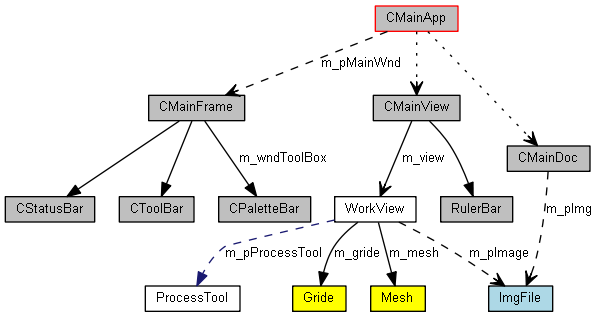
\includegraphics[width=\textwidth,height=\textheight/2,keepaspectratio=true]{dot_inline_dotgraph_2}}
\end{DoxyImageNoCaption}
\hypertarget{index_process}{}\section{Process\+Tool Hierarchy}\label{index_process}

\begin{DoxyImageNoCaption}
  \mbox{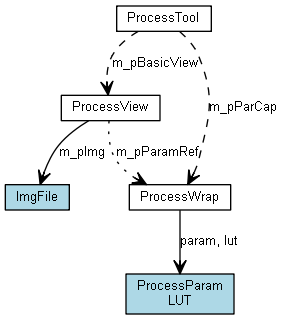
\includegraphics[width=\textwidth,height=\textheight/2,keepaspectratio=true]{dot_inline_dotgraph_3}}
\end{DoxyImageNoCaption}
\hypertarget{index_rendering}{}\section{Rendering Flow}\label{index_rendering}

\begin{DoxyImageNoCaption}
  \mbox{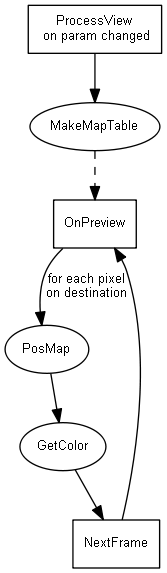
\includegraphics[width=\textwidth,height=\textheight/2,keepaspectratio=true]{dot_inline_dotgraph_4}}
\end{DoxyImageNoCaption}
 
\chapter{Hierarchical Index}
\section{Class Hierarchy}
This inheritance list is sorted roughly, but not completely, alphabetically\+:\begin{DoxyCompactList}
\item \contentsline{section}{\+\_\+\+Fec\+Param}{\pageref{struct___fec_param}}{}
\item \contentsline{section}{\+\_\+\+Gride\+Param}{\pageref{struct___gride_param}}{}
\item \contentsline{section}{\+\_\+\+Homo\+Param}{\pageref{struct___homo_param}}{}
\item \contentsline{section}{\+\_\+\+Mesh\+Control\+Data}{\pageref{struct___mesh_control_data}}{}
\item \contentsline{section}{\+\_\+\+Point\+Double}{\pageref{struct___point_double}}{}
\item C\+Dialog\begin{DoxyCompactList}
\item \contentsline{section}{C\+About\+Dlg}{\pageref{class_c_about_dlg}}{}
\item \contentsline{section}{Process\+Tool}{\pageref{class_process_tool}}{}
\begin{DoxyCompactList}
\item \contentsline{section}{Fec\+Tool}{\pageref{class_fec_tool}}{}
\item \contentsline{section}{Homo\+Tool}{\pageref{class_homo_tool}}{}
\item \contentsline{section}{Ldc\+Tool}{\pageref{class_ldc_tool}}{}
\end{DoxyCompactList}
\end{DoxyCompactList}
\item C\+Document\begin{DoxyCompactList}
\item \contentsline{section}{C\+Main\+Doc}{\pageref{class_c_main_doc}}{}
\end{DoxyCompactList}
\item C\+Frame\+Wnd\begin{DoxyCompactList}
\item \contentsline{section}{C\+Main\+Frame}{\pageref{class_c_main_frame}}{}
\end{DoxyCompactList}
\item C\+Splitter\+Wnd\begin{DoxyCompactList}
\item \contentsline{section}{C\+Ruler\+Splitter\+Wnd}{\pageref{class_c_ruler_splitter_wnd}}{}
\end{DoxyCompactList}
\item C\+Tool\+Bar\begin{DoxyCompactList}
\item \contentsline{section}{C\+Palette\+Bar}{\pageref{class_c_palette_bar}}{}
\end{DoxyCompactList}
\item C\+View\begin{DoxyCompactList}
\item \contentsline{section}{C\+Main\+View}{\pageref{class_c_main_view}}{}
\item \contentsline{section}{C\+Ruler\+Corner\+View}{\pageref{class_c_ruler_corner_view}}{}
\item \contentsline{section}{C\+Ruler\+View}{\pageref{class_c_ruler_view}}{}
\end{DoxyCompactList}
\item C\+Win\+App\begin{DoxyCompactList}
\item \contentsline{section}{C\+Main\+App}{\pageref{class_c_main_app}}{}
\end{DoxyCompactList}
\item C\+Wnd\begin{DoxyCompactList}
\item \contentsline{section}{Basic\+View}{\pageref{class_basic_view}}{}
\begin{DoxyCompactList}
\item \contentsline{section}{Process\+View}{\pageref{class_process_view}}{}
\begin{DoxyCompactList}
\item \contentsline{section}{Fec\+View}{\pageref{class_fec_view}}{}
\item \contentsline{section}{Homo\+View}{\pageref{class_homo_view}}{}
\item \contentsline{section}{Ldc\+View}{\pageref{class_ldc_view}}{}
\end{DoxyCompactList}
\item \contentsline{section}{Work\+View}{\pageref{class_work_view}}{}
\end{DoxyCompactList}
\item \contentsline{section}{Navigator}{\pageref{class_navigator}}{}
\item \contentsline{section}{Ruler\+Bar}{\pageref{class_ruler_bar}}{}
\item \contentsline{section}{Ruler\+Corner}{\pageref{class_ruler_corner}}{}
\end{DoxyCompactList}
\item \contentsline{section}{Gride}{\pageref{class_gride}}{}
\begin{DoxyCompactList}
\item \contentsline{section}{Fec\+Gride}{\pageref{class_fec_gride}}{}
\end{DoxyCompactList}
\item \contentsline{section}{Measure\+Performance}{\pageref{class_measure_performance}}{}
\item \contentsline{section}{Mesh}{\pageref{class_mesh}}{}
\item \contentsline{section}{Process\+Wrap}{\pageref{class_process_wrap}}{}
\begin{DoxyCompactList}
\item \contentsline{section}{Fec\+Wrap}{\pageref{class_fec_wrap}}{}
\item \contentsline{section}{Homo\+Wrap}{\pageref{class_homo_wrap}}{}
\item \contentsline{section}{Ldc\+Wrap}{\pageref{class_ldc_wrap}}{}
\end{DoxyCompactList}
\end{DoxyCompactList}

\chapter{Class Index}
\section{Class List}
Here are the classes, structs, unions and interfaces with brief descriptions\+:\begin{DoxyCompactList}
\item\contentsline{section}{\mbox{\hyperlink{struct___fec_param}{\+\_\+\+Fec\+Param}} \\*F\+EC processing parameters }{\pageref{struct___fec_param}}{}
\item\contentsline{section}{\mbox{\hyperlink{struct___gride_param}{\+\_\+\+Gride\+Param}} }{\pageref{struct___gride_param}}{}
\item\contentsline{section}{\mbox{\hyperlink{struct___homo_param}{\+\_\+\+Homo\+Param}} \\*Homography Matrix parameters. Q(u,v) = \mbox{[}H\mbox{]} $\ast$ P(x,y), where P is the vector of original pixels, Q is the vector of transformed pixels }{\pageref{struct___homo_param}}{}
\item\contentsline{section}{\mbox{\hyperlink{struct___mesh_control_data}{\+\_\+\+Mesh\+Control\+Data}} }{\pageref{struct___mesh_control_data}}{}
\item\contentsline{section}{\mbox{\hyperlink{struct___point_double}{\+\_\+\+Point\+Double}} \\*Double precision types of position coordinates used in L\+UT }{\pageref{struct___point_double}}{}
\item\contentsline{section}{\mbox{\hyperlink{class_basic_view}{Basic\+View}} \\*\mbox{\hyperlink{class_basic_view}{Basic\+View}} is the basic image viewer window. It handles image preview, zoom in/out, and window scrolling stuff }{\pageref{class_basic_view}}{}
\item\contentsline{section}{\mbox{\hyperlink{class_c_about_dlg}{C\+About\+Dlg}} }{\pageref{class_c_about_dlg}}{}
\item\contentsline{section}{\mbox{\hyperlink{class_c_main_app}{C\+Main\+App}} }{\pageref{class_c_main_app}}{}
\item\contentsline{section}{\mbox{\hyperlink{class_c_main_doc}{C\+Main\+Doc}} }{\pageref{class_c_main_doc}}{}
\item\contentsline{section}{\mbox{\hyperlink{class_c_main_frame}{C\+Main\+Frame}} }{\pageref{class_c_main_frame}}{}
\item\contentsline{section}{\mbox{\hyperlink{class_c_main_view}{C\+Main\+View}} }{\pageref{class_c_main_view}}{}
\item\contentsline{section}{\mbox{\hyperlink{class_c_palette_bar}{C\+Palette\+Bar}} }{\pageref{class_c_palette_bar}}{}
\item\contentsline{section}{\mbox{\hyperlink{class_c_ruler_corner_view}{C\+Ruler\+Corner\+View}} }{\pageref{class_c_ruler_corner_view}}{}
\item\contentsline{section}{\mbox{\hyperlink{class_c_ruler_splitter_wnd}{C\+Ruler\+Splitter\+Wnd}} }{\pageref{class_c_ruler_splitter_wnd}}{}
\item\contentsline{section}{\mbox{\hyperlink{class_c_ruler_view}{C\+Ruler\+View}} }{\pageref{class_c_ruler_view}}{}
\item\contentsline{section}{\mbox{\hyperlink{class_fec_gride}{Fec\+Gride}} }{\pageref{class_fec_gride}}{}
\item\contentsline{section}{\mbox{\hyperlink{class_fec_tool}{Fec\+Tool}} \\*\mbox{\hyperlink{class_fec_tool}{Fec\+Tool}} is used to control the settings of F\+EC process with UI in a dialog box. This class sends the parameters to a \mbox{\hyperlink{class_fec_view}{Fec\+View}} to display the resulted image. It also connects to a \mbox{\hyperlink{class_fec_wrap}{Fec\+Wrap}} class to maintain the F\+EC process related parameters and L\+UT data }{\pageref{class_fec_tool}}{}
\item\contentsline{section}{\mbox{\hyperlink{class_fec_view}{Fec\+View}} \\*\mbox{\hyperlink{class_fec_view}{Fec\+View}} is the image viewer for F\+EC processing image. It handles the video rendering process by the specified process. It is controlled by its process correspondent \mbox{\hyperlink{class_fec_tool}{Fec\+Tool}}. It also can display gride lines on the image window }{\pageref{class_fec_view}}{}
\item\contentsline{section}{\mbox{\hyperlink{class_fec_wrap}{Fec\+Wrap}} \\*F\+EC process parameters wrapper This class wrap F\+EC parameters and L\+UT table, as well as L\+UT generating function }{\pageref{class_fec_wrap}}{}
\item\contentsline{section}{\mbox{\hyperlink{class_gride}{Gride}} }{\pageref{class_gride}}{}
\item\contentsline{section}{\mbox{\hyperlink{class_homo_tool}{Homo\+Tool}} }{\pageref{class_homo_tool}}{}
\item\contentsline{section}{\mbox{\hyperlink{class_homo_view}{Homo\+View}} \\*\mbox{\hyperlink{class_homo_view}{Homo\+View}} is the image viewer for Homography matrix processing image. It handles the video rendering process by the specified process. It is controlled by its process correspondent \mbox{\hyperlink{class_homo_tool}{Homo\+Tool}}. It also can display gride lines on the image window }{\pageref{class_homo_view}}{}
\item\contentsline{section}{\mbox{\hyperlink{class_homo_wrap}{Homo\+Wrap}} \\*Homogrphy matrix process parameters wrapper This class wrap Homography parameters and L\+UT table, as well as L\+UT generating function }{\pageref{class_homo_wrap}}{}
\item\contentsline{section}{\mbox{\hyperlink{class_ldc_tool}{Ldc\+Tool}} \\*Ldcc\+Tool is used to control the settings of Ldc process with UI in a dialog box. This class sends the parameters to a \mbox{\hyperlink{class_fec_view}{Fec\+View}} to display the resulted image. It also connects to a \mbox{\hyperlink{class_ldc_wrap}{Ldc\+Wrap}} class to maintain the L\+DC process related parameters and L\+UT data }{\pageref{class_ldc_tool}}{}
\item\contentsline{section}{\mbox{\hyperlink{class_ldc_view}{Ldc\+View}} \\*\mbox{\hyperlink{class_ldc_view}{Ldc\+View}} is the image viewer for L\+DC processing image. It handles the video rendering process by the specified process. It is controlled by its process correspondent \mbox{\hyperlink{class_ldc_tool}{Ldc\+Tool}}. It also can display gride lines on the image window }{\pageref{class_ldc_view}}{}
\item\contentsline{section}{\mbox{\hyperlink{class_ldc_wrap}{Ldc\+Wrap}} \\*L\+DC process parameters wrapper This class wrap L\+DC parameters and L\+UT table, as well as L\+UT generating function }{\pageref{class_ldc_wrap}}{}
\item\contentsline{section}{\mbox{\hyperlink{class_measure_performance}{Measure\+Performance}} }{\pageref{class_measure_performance}}{}
\item\contentsline{section}{\mbox{\hyperlink{class_mesh}{Mesh}} \\*Draw mesh on the specified area working flow }{\pageref{class_mesh}}{}
\item\contentsline{section}{\mbox{\hyperlink{class_navigator}{Navigator}} }{\pageref{class_navigator}}{}
\item\contentsline{section}{\mbox{\hyperlink{class_process_tool}{Process\+Tool}} \\*\mbox{\hyperlink{class_process_tool}{Process\+Tool}} is the abstract class which is used to control the settings of a process with UI in a dialog box. A \mbox{\hyperlink{class_process_tool}{Process\+Tool}} class consistent of a \mbox{\hyperlink{class_process_view}{Process\+View}} member to display the processed image and a \mbox{\hyperlink{class_process_wrap}{Process\+Wrap}} class member to aintain the process related parameters and L\+UT data. \mbox{\hyperlink{class_process_tool}{Process\+Tool}} is the bridge class between \mbox{\hyperlink{class_work_view}{Work\+View}} and the Process. The application use \mbox{\hyperlink{class_process_tool}{Process\+Tool}} to access the specified process stuff }{\pageref{class_process_tool}}{}
\item\contentsline{section}{\mbox{\hyperlink{class_process_view}{Process\+View}} \\*\mbox{\hyperlink{class_process_view}{Process\+View}} is the basic image viewer for processing image viewing. It handles the video rendering process by the specified process. It is controlled by its process correspondent \mbox{\hyperlink{class_process_tool}{Process\+Tool}}. It also can display gride lines on the image window }{\pageref{class_process_view}}{}
\item\contentsline{section}{\mbox{\hyperlink{class_process_wrap}{Process\+Wrap}} \\*Wrap process parameters }{\pageref{class_process_wrap}}{}
\item\contentsline{section}{\mbox{\hyperlink{class_ruler_bar}{Ruler\+Bar}} }{\pageref{class_ruler_bar}}{}
\item\contentsline{section}{\mbox{\hyperlink{class_ruler_corner}{Ruler\+Corner}} }{\pageref{class_ruler_corner}}{}
\item\contentsline{section}{\mbox{\hyperlink{class_work_view}{Work\+View}} \\*\mbox{\hyperlink{class_work_view}{Work\+View}} is the current opened image display window. It can display gride and mesh for comparision with processed image. It also provides zooming and scrolling functions for viewing }{\pageref{class_work_view}}{}
\end{DoxyCompactList}

\chapter{File Index}
\section{File List}
Here is a list of all documented files with brief descriptions\+:\begin{DoxyCompactList}
\item\contentsline{section}{i\+Optics/\mbox{\hyperlink{_basic_view_8h}{Basic\+View.\+h}} }{\pageref{_basic_view_8h}}{}
\item\contentsline{section}{i\+Optics/\mbox{\hyperlink{common_8h}{common.\+h}} \\*This file declars process-\/related struc and data type }{\pageref{common_8h}}{}
\item\contentsline{section}{i\+Optics/\mbox{\hyperlink{_fec_tool_8h}{Fec\+Tool.\+h}} }{\pageref{_fec_tool_8h}}{}
\item\contentsline{section}{i\+Optics/\mbox{\hyperlink{_fec_view_8h}{Fec\+View.\+h}} }{\pageref{_fec_view_8h}}{}
\item\contentsline{section}{i\+Optics/{\bfseries Gride.\+h} }{\pageref{_gride_8h}}{}
\item\contentsline{section}{i\+Optics/{\bfseries Homo\+Tool.\+h} }{\pageref{_homo_tool_8h}}{}
\item\contentsline{section}{i\+Optics/\mbox{\hyperlink{_homo_view_8h}{Homo\+View.\+h}} }{\pageref{_homo_view_8h}}{}
\item\contentsline{section}{i\+Optics/{\bfseries Img\+Process.\+h} }{\pageref{_img_process_8h}}{}
\item\contentsline{section}{i\+Optics/{\bfseries i\+Optics.\+h} }{\pageref{i_optics_8h}}{}
\item\contentsline{section}{i\+Optics/\mbox{\hyperlink{_ldc_tool_8h}{Ldc\+Tool.\+h}} }{\pageref{_ldc_tool_8h}}{}
\item\contentsline{section}{i\+Optics/\mbox{\hyperlink{_ldc_view_8h}{Ldc\+View.\+h}} }{\pageref{_ldc_view_8h}}{}
\item\contentsline{section}{i\+Optics/{\bfseries Main\+Doc.\+h} }{\pageref{_main_doc_8h}}{}
\item\contentsline{section}{i\+Optics/{\bfseries Main\+Frm.\+h} }{\pageref{_main_frm_8h}}{}
\item\contentsline{section}{i\+Optics/{\bfseries Main\+View.\+h} }{\pageref{_main_view_8h}}{}
\item\contentsline{section}{i\+Optics/{\bfseries Measure\+Performance.\+h} }{\pageref{_measure_performance_8h}}{}
\item\contentsline{section}{i\+Optics/\mbox{\hyperlink{_mesh_8cpp}{Mesh.\+cpp}} \\*\mbox{\hyperlink{class_mesh}{Mesh}} is used to draw look-\/up table of image transformation, as mesh like, on an image }{\pageref{_mesh_8cpp}}{}
\item\contentsline{section}{i\+Optics/\mbox{\hyperlink{_mesh_8h}{Mesh.\+h}} }{\pageref{_mesh_8h}}{}
\item\contentsline{section}{i\+Optics/{\bfseries Navigator.\+h} }{\pageref{_navigator_8h}}{}
\item\contentsline{section}{i\+Optics/{\bfseries palette.\+h} }{\pageref{palette_8h}}{}
\item\contentsline{section}{i\+Optics/\mbox{\hyperlink{_process_tool_8h}{Process\+Tool.\+h}} }{\pageref{_process_tool_8h}}{}
\item\contentsline{section}{i\+Optics/{\bfseries Process\+View.\+h} }{\pageref{_process_view_8h}}{}
\item\contentsline{section}{i\+Optics/{\bfseries resource.\+h} }{\pageref{resource_8h}}{}
\item\contentsline{section}{i\+Optics/{\bfseries ruler.\+h} }{\pageref{ruler_8h}}{}
\item\contentsline{section}{i\+Optics/{\bfseries Ruler\+Bar.\+h} }{\pageref{_ruler_bar_8h}}{}
\item\contentsline{section}{i\+Optics/{\bfseries stdafx.\+h} }{\pageref{stdafx_8h}}{}
\item\contentsline{section}{i\+Optics/{\bfseries targetver.\+h} }{\pageref{targetver_8h}}{}
\item\contentsline{section}{i\+Optics/\mbox{\hyperlink{_work_view_8h}{Work\+View.\+h}} }{\pageref{_work_view_8h}}{}
\end{DoxyCompactList}

\chapter{Class Documentation}
\hypertarget{struct___fec_param}{}\section{\+\_\+\+Fec\+Param Struct Reference}
\label{struct___fec_param}\index{\+\_\+\+Fec\+Param@{\+\_\+\+Fec\+Param}}


F\+EC processing parameters.  




{\ttfamily \#include $<$common.\+h$>$}

\subsection*{Public Attributes}
\begin{DoxyCompactItemize}
\item 
S\+I\+ZE \mbox{\hyperlink{struct___fec_param_aa83db363e7cdb88bf398152068f373fe}{sz\+Input}}
\item 
P\+O\+I\+NT \mbox{\hyperlink{struct___fec_param_a4a9ab36b8886d09177989d8f5ad4636b}{pt\+Center}}
\item 
S\+I\+ZE \mbox{\hyperlink{struct___fec_param_aa981a92a6da32125e1b044dff603df4e}{sz\+Radius}}
\item 
float \mbox{\hyperlink{struct___fec_param_ac5bc4b6bb2ff5381458001e7106b0db7}{pitch}}
\item 
float \mbox{\hyperlink{struct___fec_param_a420253746bf3b988571baff716521f50}{yaw}}
\item 
float \mbox{\hyperlink{struct___fec_param_a519744a92fa4b5f27d8e80f4cac6d029}{roll}}
\item 
float \mbox{\hyperlink{struct___fec_param_a72350a015193ca8450c7a87f315028a4}{ratio}}
\item 
float \mbox{\hyperlink{struct___fec_param_a25e29757d04be1e6b7b1cf8709670d49}{curveH}}
\item 
float \mbox{\hyperlink{struct___fec_param_aa254903d8631ae012dc4c3d4b0ab3969}{curveV}}
\item 
float \mbox{\hyperlink{struct___fec_param_acc8b9b08bfeabd57a76ac89e7bac4a59}{fovH}}
\item 
float \mbox{\hyperlink{struct___fec_param_a5f4a6533e68132c4a9d7fdbde282ed28}{fovV}}
\item 
S\+I\+ZE \mbox{\hyperlink{struct___fec_param_a8012431882fcb79b1e4ec3291fd24f56}{sz\+Output}}
\item 
Mount\+Mode \mbox{\hyperlink{struct___fec_param_af218d4cb5ba8a680830dced86a4e1d31}{mm}}
\item 
Lens\+Type \mbox{\hyperlink{struct___fec_param_a91947fce0433e75078979f4a1b0ebc81}{lt}}
\end{DoxyCompactItemize}


\subsection{Detailed Description}
F\+EC processing parameters. 

\subsection{Member Data Documentation}
\mbox{\Hypertarget{struct___fec_param_a25e29757d04be1e6b7b1cf8709670d49}\label{struct___fec_param_a25e29757d04be1e6b7b1cf8709670d49}} 
\index{\+\_\+\+Fec\+Param@{\+\_\+\+Fec\+Param}!curveH@{curveH}}
\index{curveH@{curveH}!\+\_\+\+Fec\+Param@{\+\_\+\+Fec\+Param}}
\subsubsection{\texorpdfstring{curveH}{curveH}}
{\footnotesize\ttfamily float \+\_\+\+Fec\+Param\+::curveH}

curvature coefficient of hoizontal, upper or lower \mbox{\Hypertarget{struct___fec_param_aa254903d8631ae012dc4c3d4b0ab3969}\label{struct___fec_param_aa254903d8631ae012dc4c3d4b0ab3969}} 
\index{\+\_\+\+Fec\+Param@{\+\_\+\+Fec\+Param}!curveV@{curveV}}
\index{curveV@{curveV}!\+\_\+\+Fec\+Param@{\+\_\+\+Fec\+Param}}
\subsubsection{\texorpdfstring{curveV}{curveV}}
{\footnotesize\ttfamily float \+\_\+\+Fec\+Param\+::curveV}

curvature coefficient of vertical, lefter or righter \mbox{\Hypertarget{struct___fec_param_acc8b9b08bfeabd57a76ac89e7bac4a59}\label{struct___fec_param_acc8b9b08bfeabd57a76ac89e7bac4a59}} 
\index{\+\_\+\+Fec\+Param@{\+\_\+\+Fec\+Param}!fovH@{fovH}}
\index{fovH@{fovH}!\+\_\+\+Fec\+Param@{\+\_\+\+Fec\+Param}}
\subsubsection{\texorpdfstring{fovH}{fovH}}
{\footnotesize\ttfamily float \+\_\+\+Fec\+Param\+::fovH}

hoizontal F\+OV factor, -\/1 to 1, maps to P\+I/2$\sim$ 3\+P\+I/2, default 0 (PI) \mbox{\Hypertarget{struct___fec_param_a5f4a6533e68132c4a9d7fdbde282ed28}\label{struct___fec_param_a5f4a6533e68132c4a9d7fdbde282ed28}} 
\index{\+\_\+\+Fec\+Param@{\+\_\+\+Fec\+Param}!fovV@{fovV}}
\index{fovV@{fovV}!\+\_\+\+Fec\+Param@{\+\_\+\+Fec\+Param}}
\subsubsection{\texorpdfstring{fovV}{fovV}}
{\footnotesize\ttfamily float \+\_\+\+Fec\+Param\+::fovV}

vertical F\+OV factor, -\/1 to 1, maps to P\+I/2$\sim$ 3\+P\+I/2, default 0 (PI) \mbox{\Hypertarget{struct___fec_param_a91947fce0433e75078979f4a1b0ebc81}\label{struct___fec_param_a91947fce0433e75078979f4a1b0ebc81}} 
\index{\+\_\+\+Fec\+Param@{\+\_\+\+Fec\+Param}!lt@{lt}}
\index{lt@{lt}!\+\_\+\+Fec\+Param@{\+\_\+\+Fec\+Param}}
\subsubsection{\texorpdfstring{lt}{lt}}
{\footnotesize\ttfamily Lens\+Type \+\_\+\+Fec\+Param\+::lt}

lens type \mbox{\Hypertarget{struct___fec_param_af218d4cb5ba8a680830dced86a4e1d31}\label{struct___fec_param_af218d4cb5ba8a680830dced86a4e1d31}} 
\index{\+\_\+\+Fec\+Param@{\+\_\+\+Fec\+Param}!mm@{mm}}
\index{mm@{mm}!\+\_\+\+Fec\+Param@{\+\_\+\+Fec\+Param}}
\subsubsection{\texorpdfstring{mm}{mm}}
{\footnotesize\ttfamily Mount\+Mode \+\_\+\+Fec\+Param\+::mm}

mount type \mbox{\Hypertarget{struct___fec_param_ac5bc4b6bb2ff5381458001e7106b0db7}\label{struct___fec_param_ac5bc4b6bb2ff5381458001e7106b0db7}} 
\index{\+\_\+\+Fec\+Param@{\+\_\+\+Fec\+Param}!pitch@{pitch}}
\index{pitch@{pitch}!\+\_\+\+Fec\+Param@{\+\_\+\+Fec\+Param}}
\subsubsection{\texorpdfstring{pitch}{pitch}}
{\footnotesize\ttfamily float \+\_\+\+Fec\+Param\+::pitch}

pitch angle in radiun \mbox{\Hypertarget{struct___fec_param_a4a9ab36b8886d09177989d8f5ad4636b}\label{struct___fec_param_a4a9ab36b8886d09177989d8f5ad4636b}} 
\index{\+\_\+\+Fec\+Param@{\+\_\+\+Fec\+Param}!pt\+Center@{pt\+Center}}
\index{pt\+Center@{pt\+Center}!\+\_\+\+Fec\+Param@{\+\_\+\+Fec\+Param}}
\subsubsection{\texorpdfstring{pt\+Center}{ptCenter}}
{\footnotesize\ttfamily P\+O\+I\+NT \+\_\+\+Fec\+Param\+::pt\+Center}

symmetry center of image \mbox{\Hypertarget{struct___fec_param_a72350a015193ca8450c7a87f315028a4}\label{struct___fec_param_a72350a015193ca8450c7a87f315028a4}} 
\index{\+\_\+\+Fec\+Param@{\+\_\+\+Fec\+Param}!ratio@{ratio}}
\index{ratio@{ratio}!\+\_\+\+Fec\+Param@{\+\_\+\+Fec\+Param}}
\subsubsection{\texorpdfstring{ratio}{ratio}}
{\footnotesize\ttfamily float \+\_\+\+Fec\+Param\+::ratio}

ratio of remap from small sphere to big sphere \mbox{\Hypertarget{struct___fec_param_a519744a92fa4b5f27d8e80f4cac6d029}\label{struct___fec_param_a519744a92fa4b5f27d8e80f4cac6d029}} 
\index{\+\_\+\+Fec\+Param@{\+\_\+\+Fec\+Param}!roll@{roll}}
\index{roll@{roll}!\+\_\+\+Fec\+Param@{\+\_\+\+Fec\+Param}}
\subsubsection{\texorpdfstring{roll}{roll}}
{\footnotesize\ttfamily float \+\_\+\+Fec\+Param\+::roll}

rotate with respect to z-\/axis \mbox{\Hypertarget{struct___fec_param_aa83db363e7cdb88bf398152068f373fe}\label{struct___fec_param_aa83db363e7cdb88bf398152068f373fe}} 
\index{\+\_\+\+Fec\+Param@{\+\_\+\+Fec\+Param}!sz\+Input@{sz\+Input}}
\index{sz\+Input@{sz\+Input}!\+\_\+\+Fec\+Param@{\+\_\+\+Fec\+Param}}
\subsubsection{\texorpdfstring{sz\+Input}{szInput}}
{\footnotesize\ttfamily S\+I\+ZE \+\_\+\+Fec\+Param\+::sz\+Input}

input image size \mbox{\Hypertarget{struct___fec_param_a8012431882fcb79b1e4ec3291fd24f56}\label{struct___fec_param_a8012431882fcb79b1e4ec3291fd24f56}} 
\index{\+\_\+\+Fec\+Param@{\+\_\+\+Fec\+Param}!sz\+Output@{sz\+Output}}
\index{sz\+Output@{sz\+Output}!\+\_\+\+Fec\+Param@{\+\_\+\+Fec\+Param}}
\subsubsection{\texorpdfstring{sz\+Output}{szOutput}}
{\footnotesize\ttfamily S\+I\+ZE \+\_\+\+Fec\+Param\+::sz\+Output}

desired output image size \mbox{\Hypertarget{struct___fec_param_aa981a92a6da32125e1b044dff603df4e}\label{struct___fec_param_aa981a92a6da32125e1b044dff603df4e}} 
\index{\+\_\+\+Fec\+Param@{\+\_\+\+Fec\+Param}!sz\+Radius@{sz\+Radius}}
\index{sz\+Radius@{sz\+Radius}!\+\_\+\+Fec\+Param@{\+\_\+\+Fec\+Param}}
\subsubsection{\texorpdfstring{sz\+Radius}{szRadius}}
{\footnotesize\ttfamily S\+I\+ZE \+\_\+\+Fec\+Param\+::sz\+Radius}

radius of fisheye lens, in pixels \mbox{\Hypertarget{struct___fec_param_a420253746bf3b988571baff716521f50}\label{struct___fec_param_a420253746bf3b988571baff716521f50}} 
\index{\+\_\+\+Fec\+Param@{\+\_\+\+Fec\+Param}!yaw@{yaw}}
\index{yaw@{yaw}!\+\_\+\+Fec\+Param@{\+\_\+\+Fec\+Param}}
\subsubsection{\texorpdfstring{yaw}{yaw}}
{\footnotesize\ttfamily float \+\_\+\+Fec\+Param\+::yaw}

rotate with respect to y-\/axis 

The documentation for this struct was generated from the following file\+:\begin{DoxyCompactItemize}
\item 
i\+Optics/\mbox{\hyperlink{common_8h}{common.\+h}}\end{DoxyCompactItemize}

\hypertarget{struct___gride_param}{}\section{\+\_\+\+Gride\+Param Struct Reference}
\label{struct___gride_param}\index{\+\_\+\+Gride\+Param@{\+\_\+\+Gride\+Param}}
\subsection*{Public Attributes}
\begin{DoxyCompactItemize}
\item 
\mbox{\Hypertarget{struct___gride_param_a54db6ff69ed97260c3e5f65e63a8c517}\label{struct___gride_param_a54db6ff69ed97260c3e5f65e63a8c517}} 
int {\bfseries n\+Interval}
\item 
\mbox{\Hypertarget{struct___gride_param_a6de4db533b739d137bd0907050d2991e}\label{struct___gride_param_a6de4db533b739d137bd0907050d2991e}} 
int {\bfseries n\+Divider}
\end{DoxyCompactItemize}


The documentation for this struct was generated from the following file\+:\begin{DoxyCompactItemize}
\item 
i\+Optics/Gride.\+h\end{DoxyCompactItemize}

\hypertarget{struct___homo_param}{}\section{\+\_\+\+Homo\+Param Struct Reference}
\label{struct___homo_param}\index{\+\_\+\+Homo\+Param@{\+\_\+\+Homo\+Param}}


Homography Matrix parameters. Q(u,v) = \mbox{[}H\mbox{]} $\ast$ P(x,y), where P is the vector of original pixels, Q is the vector of transformed pixels.  




{\ttfamily \#include $<$common.\+h$>$}

\subsection*{Public Attributes}
\begin{DoxyCompactItemize}
\item 
S\+I\+ZE \mbox{\hyperlink{struct___homo_param_ad4ae576eb7ce7447d24027227f39212e}{sz\+Input}}
\item 
S\+I\+ZE \mbox{\hyperlink{struct___homo_param_a2867aab6560d4a6ed0299cb425acdd75}{sz\+Output}}
\item 
float \mbox{\hyperlink{struct___homo_param_a115e689b4a04a4c084199abd52ada276}{a}}
\item 
float \mbox{\hyperlink{struct___homo_param_a6bf6d63208b553c9b23389b4757062ba}{b}}
\item 
float \mbox{\hyperlink{struct___homo_param_a14f426f73e6461dce1be2019115601c0}{c}}
\item 
float \mbox{\hyperlink{struct___homo_param_afb50d3702e446ae39dc7fe35011049f4}{d}}
\item 
float \mbox{\hyperlink{struct___homo_param_ab88060be804013eb2a53a79aa567acac}{e}}
\item 
float \mbox{\hyperlink{struct___homo_param_ab2ae30e36db1679302959fa47316837e}{f}}
\item 
float \mbox{\hyperlink{struct___homo_param_a7707b9cdca4b270d8dfbc0c183577e2a}{g}}
\item 
float \mbox{\hyperlink{struct___homo_param_ae9b878884bff7393ef6b9653610c35c6}{h}}
\end{DoxyCompactItemize}


\subsection{Detailed Description}
Homography Matrix parameters. Q(u,v) = \mbox{[}H\mbox{]} $\ast$ P(x,y), where P is the vector of original pixels, Q is the vector of transformed pixels. 

\hypertarget{struct___homo_param_multi_row}{}
\tabulinesep=1mm
\begin{longtabu} spread 0pt [c]{*{3}{|X[-1]}|}
\caption{Coefficents}\label{struct___homo_param_multi_row}\\
\hline
\rowcolor{\tableheadbgcolor}\textbf{ Q }&\textbf{ \mbox{[}H\mbox{]} }&\textbf{ P }\\\cline{1-3}
\endfirsthead
\hline
\endfoot
\hline
\rowcolor{\tableheadbgcolor}\textbf{ Q }&\textbf{ \mbox{[}H\mbox{]} }&\textbf{ P }\\\cline{1-3}
\endhead
u&a,b,c&x \\\cline{1-3}
v&d,e,f&y \\\cline{1-3}
1&g,h,1&1 \\\cline{1-3}
\end{longtabu}


\subsection{Member Data Documentation}
\mbox{\Hypertarget{struct___homo_param_a115e689b4a04a4c084199abd52ada276}\label{struct___homo_param_a115e689b4a04a4c084199abd52ada276}} 
\index{\+\_\+\+Homo\+Param@{\+\_\+\+Homo\+Param}!a@{a}}
\index{a@{a}!\+\_\+\+Homo\+Param@{\+\_\+\+Homo\+Param}}
\subsubsection{\texorpdfstring{a}{a}}
{\footnotesize\ttfamily float \+\_\+\+Homo\+Param\+::a}

Homography Matrix coef. h11 \mbox{\Hypertarget{struct___homo_param_a6bf6d63208b553c9b23389b4757062ba}\label{struct___homo_param_a6bf6d63208b553c9b23389b4757062ba}} 
\index{\+\_\+\+Homo\+Param@{\+\_\+\+Homo\+Param}!b@{b}}
\index{b@{b}!\+\_\+\+Homo\+Param@{\+\_\+\+Homo\+Param}}
\subsubsection{\texorpdfstring{b}{b}}
{\footnotesize\ttfamily float \+\_\+\+Homo\+Param\+::b}

Homography Matrix coef. h12 \mbox{\Hypertarget{struct___homo_param_a14f426f73e6461dce1be2019115601c0}\label{struct___homo_param_a14f426f73e6461dce1be2019115601c0}} 
\index{\+\_\+\+Homo\+Param@{\+\_\+\+Homo\+Param}!c@{c}}
\index{c@{c}!\+\_\+\+Homo\+Param@{\+\_\+\+Homo\+Param}}
\subsubsection{\texorpdfstring{c}{c}}
{\footnotesize\ttfamily float \+\_\+\+Homo\+Param\+::c}

Homography Matrix coef. h13 \mbox{\Hypertarget{struct___homo_param_afb50d3702e446ae39dc7fe35011049f4}\label{struct___homo_param_afb50d3702e446ae39dc7fe35011049f4}} 
\index{\+\_\+\+Homo\+Param@{\+\_\+\+Homo\+Param}!d@{d}}
\index{d@{d}!\+\_\+\+Homo\+Param@{\+\_\+\+Homo\+Param}}
\subsubsection{\texorpdfstring{d}{d}}
{\footnotesize\ttfamily float \+\_\+\+Homo\+Param\+::d}

Homography Matrix coef. h21 \mbox{\Hypertarget{struct___homo_param_ab88060be804013eb2a53a79aa567acac}\label{struct___homo_param_ab88060be804013eb2a53a79aa567acac}} 
\index{\+\_\+\+Homo\+Param@{\+\_\+\+Homo\+Param}!e@{e}}
\index{e@{e}!\+\_\+\+Homo\+Param@{\+\_\+\+Homo\+Param}}
\subsubsection{\texorpdfstring{e}{e}}
{\footnotesize\ttfamily float \+\_\+\+Homo\+Param\+::e}

Homography Matrix coef. h22 \mbox{\Hypertarget{struct___homo_param_ab2ae30e36db1679302959fa47316837e}\label{struct___homo_param_ab2ae30e36db1679302959fa47316837e}} 
\index{\+\_\+\+Homo\+Param@{\+\_\+\+Homo\+Param}!f@{f}}
\index{f@{f}!\+\_\+\+Homo\+Param@{\+\_\+\+Homo\+Param}}
\subsubsection{\texorpdfstring{f}{f}}
{\footnotesize\ttfamily float \+\_\+\+Homo\+Param\+::f}

Homography Matrix coef. h23 \mbox{\Hypertarget{struct___homo_param_a7707b9cdca4b270d8dfbc0c183577e2a}\label{struct___homo_param_a7707b9cdca4b270d8dfbc0c183577e2a}} 
\index{\+\_\+\+Homo\+Param@{\+\_\+\+Homo\+Param}!g@{g}}
\index{g@{g}!\+\_\+\+Homo\+Param@{\+\_\+\+Homo\+Param}}
\subsubsection{\texorpdfstring{g}{g}}
{\footnotesize\ttfamily float \+\_\+\+Homo\+Param\+::g}

Homography Matrix coef. h31 \mbox{\Hypertarget{struct___homo_param_ae9b878884bff7393ef6b9653610c35c6}\label{struct___homo_param_ae9b878884bff7393ef6b9653610c35c6}} 
\index{\+\_\+\+Homo\+Param@{\+\_\+\+Homo\+Param}!h@{h}}
\index{h@{h}!\+\_\+\+Homo\+Param@{\+\_\+\+Homo\+Param}}
\subsubsection{\texorpdfstring{h}{h}}
{\footnotesize\ttfamily float \+\_\+\+Homo\+Param\+::h}

Homography Matrix coef. h32 \mbox{\Hypertarget{struct___homo_param_ad4ae576eb7ce7447d24027227f39212e}\label{struct___homo_param_ad4ae576eb7ce7447d24027227f39212e}} 
\index{\+\_\+\+Homo\+Param@{\+\_\+\+Homo\+Param}!sz\+Input@{sz\+Input}}
\index{sz\+Input@{sz\+Input}!\+\_\+\+Homo\+Param@{\+\_\+\+Homo\+Param}}
\subsubsection{\texorpdfstring{sz\+Input}{szInput}}
{\footnotesize\ttfamily S\+I\+ZE \+\_\+\+Homo\+Param\+::sz\+Input}

input image size \mbox{\Hypertarget{struct___homo_param_a2867aab6560d4a6ed0299cb425acdd75}\label{struct___homo_param_a2867aab6560d4a6ed0299cb425acdd75}} 
\index{\+\_\+\+Homo\+Param@{\+\_\+\+Homo\+Param}!sz\+Output@{sz\+Output}}
\index{sz\+Output@{sz\+Output}!\+\_\+\+Homo\+Param@{\+\_\+\+Homo\+Param}}
\subsubsection{\texorpdfstring{sz\+Output}{szOutput}}
{\footnotesize\ttfamily S\+I\+ZE \+\_\+\+Homo\+Param\+::sz\+Output}

desired output image size 

The documentation for this struct was generated from the following file\+:\begin{DoxyCompactItemize}
\item 
i\+Optics/\mbox{\hyperlink{common_8h}{common.\+h}}\end{DoxyCompactItemize}

\hypertarget{struct___mesh_control_data}{}\section{\+\_\+\+Mesh\+Control\+Data Struct Reference}
\label{struct___mesh_control_data}\index{\+\_\+\+Mesh\+Control\+Data@{\+\_\+\+Mesh\+Control\+Data}}
\subsection*{Public Attributes}
\begin{DoxyCompactItemize}
\item 
int \mbox{\hyperlink{struct___mesh_control_data_a3ce4c585ce3b8c434736a6aeafbf8191}{column}}
\item 
int \mbox{\hyperlink{struct___mesh_control_data_a282572be6466c1e1761fb9fa56846741}{row}}
\item 
\mbox{\hyperlink{struct___point_double}{Point\+Double}} $\ast$ \mbox{\hyperlink{struct___mesh_control_data_a9477d1f3207021a27501dbae79940c0a}{p\+Cp}}
\end{DoxyCompactItemize}


\subsection{Member Data Documentation}
\mbox{\Hypertarget{struct___mesh_control_data_a3ce4c585ce3b8c434736a6aeafbf8191}\label{struct___mesh_control_data_a3ce4c585ce3b8c434736a6aeafbf8191}} 
\index{\+\_\+\+Mesh\+Control\+Data@{\+\_\+\+Mesh\+Control\+Data}!column@{column}}
\index{column@{column}!\+\_\+\+Mesh\+Control\+Data@{\+\_\+\+Mesh\+Control\+Data}}
\subsubsection{\texorpdfstring{column}{column}}
{\footnotesize\ttfamily int \+\_\+\+Mesh\+Control\+Data\+::column}

number of column \mbox{\Hypertarget{struct___mesh_control_data_a9477d1f3207021a27501dbae79940c0a}\label{struct___mesh_control_data_a9477d1f3207021a27501dbae79940c0a}} 
\index{\+\_\+\+Mesh\+Control\+Data@{\+\_\+\+Mesh\+Control\+Data}!p\+Cp@{p\+Cp}}
\index{p\+Cp@{p\+Cp}!\+\_\+\+Mesh\+Control\+Data@{\+\_\+\+Mesh\+Control\+Data}}
\subsubsection{\texorpdfstring{p\+Cp}{pCp}}
{\footnotesize\ttfamily \mbox{\hyperlink{struct___point_double}{Point\+Double}}$\ast$ \+\_\+\+Mesh\+Control\+Data\+::p\+Cp}

start address of the control data \mbox{\Hypertarget{struct___mesh_control_data_a282572be6466c1e1761fb9fa56846741}\label{struct___mesh_control_data_a282572be6466c1e1761fb9fa56846741}} 
\index{\+\_\+\+Mesh\+Control\+Data@{\+\_\+\+Mesh\+Control\+Data}!row@{row}}
\index{row@{row}!\+\_\+\+Mesh\+Control\+Data@{\+\_\+\+Mesh\+Control\+Data}}
\subsubsection{\texorpdfstring{row}{row}}
{\footnotesize\ttfamily int \+\_\+\+Mesh\+Control\+Data\+::row}

number of row 

The documentation for this struct was generated from the following file\+:\begin{DoxyCompactItemize}
\item 
i\+Optics/\mbox{\hyperlink{_mesh_8h}{Mesh.\+h}}\end{DoxyCompactItemize}

\hypertarget{struct___point_double}{}\section{\+\_\+\+Point\+Double Struct Reference}
\label{struct___point_double}\index{\+\_\+\+Point\+Double@{\+\_\+\+Point\+Double}}


double precision types of position coordinates used in L\+UT  




{\ttfamily \#include $<$common.\+h$>$}

\subsection*{Public Attributes}
\begin{DoxyCompactItemize}
\item 
double \mbox{\hyperlink{struct___point_double_aa250ab1da28280804dba8c1116e0586f}{x}}
\item 
double \mbox{\hyperlink{struct___point_double_ab9150c29d5a2399ef62b28b7a8b01ea1}{y}}
\end{DoxyCompactItemize}


\subsection{Detailed Description}
double precision types of position coordinates used in L\+UT 

\subsection{Member Data Documentation}
\mbox{\Hypertarget{struct___point_double_aa250ab1da28280804dba8c1116e0586f}\label{struct___point_double_aa250ab1da28280804dba8c1116e0586f}} 
\index{\+\_\+\+Point\+Double@{\+\_\+\+Point\+Double}!x@{x}}
\index{x@{x}!\+\_\+\+Point\+Double@{\+\_\+\+Point\+Double}}
\subsubsection{\texorpdfstring{x}{x}}
{\footnotesize\ttfamily double \+\_\+\+Point\+Double\+::x}

x-\/coordinates \mbox{\Hypertarget{struct___point_double_ab9150c29d5a2399ef62b28b7a8b01ea1}\label{struct___point_double_ab9150c29d5a2399ef62b28b7a8b01ea1}} 
\index{\+\_\+\+Point\+Double@{\+\_\+\+Point\+Double}!y@{y}}
\index{y@{y}!\+\_\+\+Point\+Double@{\+\_\+\+Point\+Double}}
\subsubsection{\texorpdfstring{y}{y}}
{\footnotesize\ttfamily double \+\_\+\+Point\+Double\+::y}

y-\/coordinates 

The documentation for this struct was generated from the following file\+:\begin{DoxyCompactItemize}
\item 
i\+Optics/\mbox{\hyperlink{common_8h}{common.\+h}}\end{DoxyCompactItemize}

\hypertarget{class_basic_view}{}\section{Basic\+View Class Reference}
\label{class_basic_view}\index{Basic\+View@{Basic\+View}}


\mbox{\hyperlink{class_basic_view}{Basic\+View}} is the basic image viewer window. It handles image preview, zoom in/out, and window scrolling stuff.  




{\ttfamily \#include $<$Basic\+View.\+h$>$}

Inheritance diagram for Basic\+View\+:\begin{figure}[H]
\begin{center}
\leavevmode
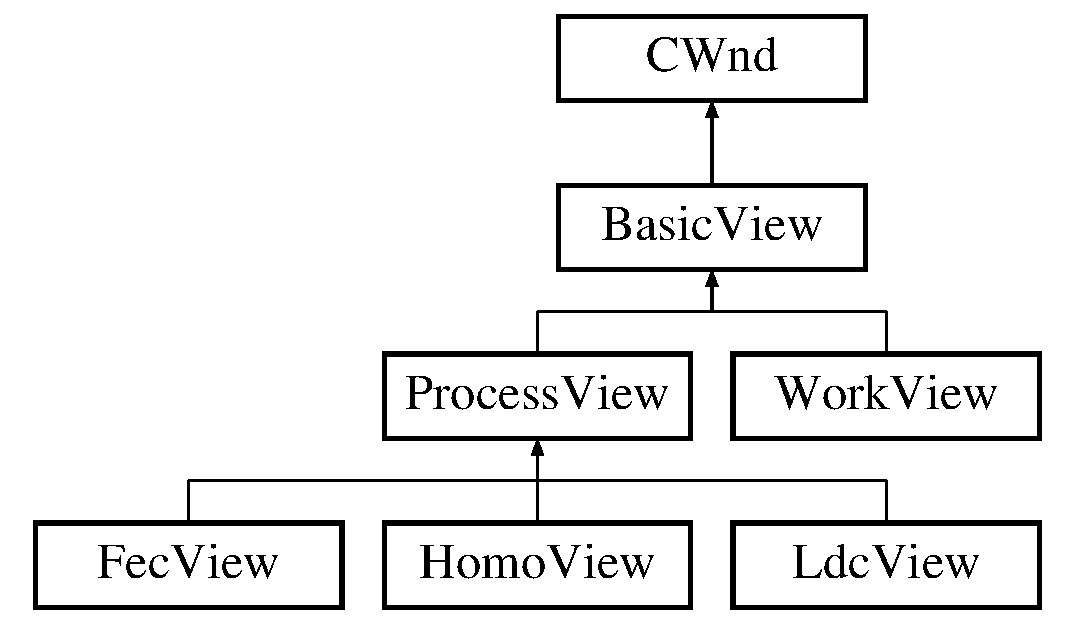
\includegraphics[height=4.000000cm]{class_basic_view}
\end{center}
\end{figure}
\subsection*{Public Member Functions}
\begin{DoxyCompactItemize}
\item 
\mbox{\Hypertarget{class_basic_view_ad48fb56fa9b09b92f541a79c66901cea}\label{class_basic_view_ad48fb56fa9b09b92f541a79c66901cea}} 
virtual void {\bfseries Set\+Img\+File} (Img\+File $\ast$p\+Img)
\item 
\mbox{\Hypertarget{class_basic_view_a6efb4e96e3f56d57bca547016980e12c}\label{class_basic_view_a6efb4e96e3f56d57bca547016980e12c}} 
Img\+File $\ast$ {\bfseries Get\+Img\+File} ()
\item 
\mbox{\Hypertarget{class_basic_view_a4d5fefc55235b1b84bcf6cfe5c9f140d}\label{class_basic_view_a4d5fefc55235b1b84bcf6cfe5c9f140d}} 
void {\bfseries Draw\+Image} (C\+DC $\ast$p\+DC)
\item 
\mbox{\Hypertarget{class_basic_view_a70a63eea47d1e23d50f67c62080e42c5}\label{class_basic_view_a70a63eea47d1e23d50f67c62080e42c5}} 
virtual B\+O\+OL {\bfseries Create} (L\+P\+C\+T\+S\+TR sz\+Name, C\+Wnd $\ast$p\+Parent\+Wnd, B\+O\+OL b\+Popup)
\item 
\mbox{\Hypertarget{class_basic_view_af13f4ac91b170f02e60f1ff231402ac2}\label{class_basic_view_af13f4ac91b170f02e60f1ff231402ac2}} 
virtual void {\bfseries Update\+Scrollbar\+Position} ()
\item 
virtual void \mbox{\hyperlink{class_basic_view_ab553e969a295d6d6933a7a701ade79bc}{Set\+Param}} (void $\ast$p\+Param)
\item 
\mbox{\Hypertarget{class_basic_view_a495262f5dc8aa19a66a11f28fd73ca3b}\label{class_basic_view_a495262f5dc8aa19a66a11f28fd73ca3b}} 
afx\+\_\+msg B\+O\+OL {\bfseries On\+Erase\+Bkgnd} (C\+DC $\ast$p\+DC)
\item 
\mbox{\Hypertarget{class_basic_view_ae459b872e7b726d8e1c23ad0b7516a08}\label{class_basic_view_ae459b872e7b726d8e1c23ad0b7516a08}} 
afx\+\_\+msg void {\bfseries On\+Paint} ()
\item 
\mbox{\Hypertarget{class_basic_view_a99599b49df57fdb7526d97dd9cbc63dd}\label{class_basic_view_a99599b49df57fdb7526d97dd9cbc63dd}} 
afx\+\_\+msg void {\bfseries On\+Size} (U\+I\+NT n\+Type, int cx, int cy)
\item 
\mbox{\Hypertarget{class_basic_view_a8f9fbf9908c3e133b732fca6048f776a}\label{class_basic_view_a8f9fbf9908c3e133b732fca6048f776a}} 
afx\+\_\+msg void {\bfseries On\+H\+Scroll} (U\+I\+NT n\+S\+B\+Code, U\+I\+NT n\+Pos, C\+Scroll\+Bar $\ast$p\+Scroll\+Bar)
\item 
\mbox{\Hypertarget{class_basic_view_aa15ef76fc3123761dabf6c26d2079a44}\label{class_basic_view_aa15ef76fc3123761dabf6c26d2079a44}} 
afx\+\_\+msg void {\bfseries On\+V\+Scroll} (U\+I\+NT n\+S\+B\+Code, U\+I\+NT n\+Pos, C\+Scroll\+Bar $\ast$p\+Scroll\+Bar)
\item 
\mbox{\Hypertarget{class_basic_view_a80315db783abe2477eda76b66750b571}\label{class_basic_view_a80315db783abe2477eda76b66750b571}} 
afx\+\_\+msg void {\bfseries On\+View\+Zoomin} ()
\item 
\mbox{\Hypertarget{class_basic_view_abdf4441d048617debebd65959130c4ea}\label{class_basic_view_abdf4441d048617debebd65959130c4ea}} 
afx\+\_\+msg void {\bfseries On\+Update\+View\+Zoomin} (C\+Cmd\+UI $\ast$p\+Cmd\+UI)
\item 
\mbox{\Hypertarget{class_basic_view_a6683be2d4eaf00df6bf3c865de183719}\label{class_basic_view_a6683be2d4eaf00df6bf3c865de183719}} 
afx\+\_\+msg void {\bfseries On\+View\+Zoomout} ()
\item 
\mbox{\Hypertarget{class_basic_view_a8413f54e94417ffd14feb39687c02e3a}\label{class_basic_view_a8413f54e94417ffd14feb39687c02e3a}} 
afx\+\_\+msg void {\bfseries On\+Update\+View\+Zoomout} (C\+Cmd\+UI $\ast$p\+Cmd\+UI)
\item 
\mbox{\Hypertarget{class_basic_view_a7e588e703875860f0c83de89c1256b9f}\label{class_basic_view_a7e588e703875860f0c83de89c1256b9f}} 
afx\+\_\+msg void {\bfseries On\+Close} ()
\end{DoxyCompactItemize}
\subsection*{Static Public Attributes}
\begin{DoxyCompactItemize}
\item 
static int \mbox{\hyperlink{class_basic_view_ad66db924d3a8a6937720a656336825a7}{Z\+O\+O\+M\+\_\+\+F\+A\+C\+T\+OR}} \mbox{[}M\+A\+X\+\_\+\+Z\+O\+OM\mbox{]} = \{ 10, 25, 33, 50, 75, 100,150, 200, 300, 400\}
\end{DoxyCompactItemize}
\subsection*{Protected Member Functions}
\begin{DoxyCompactItemize}
\item 
\mbox{\Hypertarget{class_basic_view_aafdbf24eb9c7260ac8c51c05839b5dd8}\label{class_basic_view_aafdbf24eb9c7260ac8c51c05839b5dd8}} 
virtual void {\bfseries Post\+Nc\+Destroy} ()
\item 
\mbox{\Hypertarget{class_basic_view_a2fa0648d41595e81c91cc58dbea5488f}\label{class_basic_view_a2fa0648d41595e81c91cc58dbea5488f}} 
void {\bfseries Doc\+To\+View\+Port} (S\+I\+ZE \&size)
\item 
\mbox{\Hypertarget{class_basic_view_a948bff6deaaa0d5a546dd7bb6c063d79}\label{class_basic_view_a948bff6deaaa0d5a546dd7bb6c063d79}} 
void {\bfseries Doc\+To\+View\+Port} (R\+E\+CT \&rect)
\item 
\mbox{\Hypertarget{class_basic_view_aba477b0400f6152ee6971142eba519a6}\label{class_basic_view_aba477b0400f6152ee6971142eba519a6}} 
void {\bfseries View\+Port\+To\+Doc} (S\+I\+ZE \&size)
\item 
\mbox{\Hypertarget{class_basic_view_abf35d7d7d7ae89a8e5ff607111be6167}\label{class_basic_view_abf35d7d7d7ae89a8e5ff607111be6167}} 
void {\bfseries View\+Port\+To\+Doc} (R\+E\+CT \&rect)
\item 
\mbox{\Hypertarget{class_basic_view_a896292cd23b8fa853fcf1451e5949d33}\label{class_basic_view_a896292cd23b8fa853fcf1451e5949d33}} 
void {\bfseries Calculate\+Rects} ()
\end{DoxyCompactItemize}
\subsection*{Protected Attributes}
\begin{DoxyCompactItemize}
\item 
int \mbox{\hyperlink{class_basic_view_a45c68c0cbfcd5275bed1d76af7272c22}{m\+\_\+n\+Zoom\+Factor}}
\item 
R\+E\+CT \mbox{\hyperlink{class_basic_view_ae0c220c7659c120bae97c43e5e79cf3f}{m\+\_\+rc\+Port}}
\item 
S\+I\+ZE \mbox{\hyperlink{class_basic_view_a576f84883374c4ca07a7071967434396}{m\+\_\+sz\+Canvas}}
\item 
R\+E\+CT \mbox{\hyperlink{class_basic_view_a9d8a549c1bcfc0e077f3d68c326a7cab}{m\+\_\+rc\+Image}}
\item 
Img\+File $\ast$ \mbox{\hyperlink{class_basic_view_a4b8c2fb4f3b0d69dcc227947b8933629}{m\+\_\+p\+Image}}
\end{DoxyCompactItemize}


\subsection{Detailed Description}
\mbox{\hyperlink{class_basic_view}{Basic\+View}} is the basic image viewer window. It handles image preview, zoom in/out, and window scrolling stuff. 

\subsection{Member Function Documentation}
\mbox{\Hypertarget{class_basic_view_ab553e969a295d6d6933a7a701ade79bc}\label{class_basic_view_ab553e969a295d6d6933a7a701ade79bc}} 
\index{Basic\+View@{Basic\+View}!Set\+Param@{Set\+Param}}
\index{Set\+Param@{Set\+Param}!Basic\+View@{Basic\+View}}
\subsubsection{\texorpdfstring{Set\+Param()}{SetParam()}}
{\footnotesize\ttfamily virtual void Basic\+View\+::\+Set\+Param (\begin{DoxyParamCaption}\item[{void $\ast$}]{p\+Param }\end{DoxyParamCaption})\hspace{0.3cm}{\ttfamily [inline]}, {\ttfamily [virtual]}}

setup class dependent parameters 

\subsection{Member Data Documentation}
\mbox{\Hypertarget{class_basic_view_a45c68c0cbfcd5275bed1d76af7272c22}\label{class_basic_view_a45c68c0cbfcd5275bed1d76af7272c22}} 
\index{Basic\+View@{Basic\+View}!m\+\_\+n\+Zoom\+Factor@{m\+\_\+n\+Zoom\+Factor}}
\index{m\+\_\+n\+Zoom\+Factor@{m\+\_\+n\+Zoom\+Factor}!Basic\+View@{Basic\+View}}
\subsubsection{\texorpdfstring{m\+\_\+n\+Zoom\+Factor}{m\_nZoomFactor}}
{\footnotesize\ttfamily int Basic\+View\+::m\+\_\+n\+Zoom\+Factor\hspace{0.3cm}{\ttfamily [protected]}}

current zoom factor index \mbox{\Hypertarget{class_basic_view_a4b8c2fb4f3b0d69dcc227947b8933629}\label{class_basic_view_a4b8c2fb4f3b0d69dcc227947b8933629}} 
\index{Basic\+View@{Basic\+View}!m\+\_\+p\+Image@{m\+\_\+p\+Image}}
\index{m\+\_\+p\+Image@{m\+\_\+p\+Image}!Basic\+View@{Basic\+View}}
\subsubsection{\texorpdfstring{m\+\_\+p\+Image}{m\_pImage}}
{\footnotesize\ttfamily Img\+File$\ast$ Basic\+View\+::m\+\_\+p\+Image\hspace{0.3cm}{\ttfamily [protected]}}

The image to be displayed in the window \mbox{\Hypertarget{class_basic_view_a9d8a549c1bcfc0e077f3d68c326a7cab}\label{class_basic_view_a9d8a549c1bcfc0e077f3d68c326a7cab}} 
\index{Basic\+View@{Basic\+View}!m\+\_\+rc\+Image@{m\+\_\+rc\+Image}}
\index{m\+\_\+rc\+Image@{m\+\_\+rc\+Image}!Basic\+View@{Basic\+View}}
\subsubsection{\texorpdfstring{m\+\_\+rc\+Image}{m\_rcImage}}
{\footnotesize\ttfamily R\+E\+CT Basic\+View\+::m\+\_\+rc\+Image\hspace{0.3cm}{\ttfamily [protected]}}

location of zoomed image on canvas \mbox{\Hypertarget{class_basic_view_ae0c220c7659c120bae97c43e5e79cf3f}\label{class_basic_view_ae0c220c7659c120bae97c43e5e79cf3f}} 
\index{Basic\+View@{Basic\+View}!m\+\_\+rc\+Port@{m\+\_\+rc\+Port}}
\index{m\+\_\+rc\+Port@{m\+\_\+rc\+Port}!Basic\+View@{Basic\+View}}
\subsubsection{\texorpdfstring{m\+\_\+rc\+Port}{m\_rcPort}}
{\footnotesize\ttfamily R\+E\+CT Basic\+View\+::m\+\_\+rc\+Port\hspace{0.3cm}{\ttfamily [protected]}}

he display area in zoomed image. top-\/left is scroll thumb poition \mbox{\Hypertarget{class_basic_view_a576f84883374c4ca07a7071967434396}\label{class_basic_view_a576f84883374c4ca07a7071967434396}} 
\index{Basic\+View@{Basic\+View}!m\+\_\+sz\+Canvas@{m\+\_\+sz\+Canvas}}
\index{m\+\_\+sz\+Canvas@{m\+\_\+sz\+Canvas}!Basic\+View@{Basic\+View}}
\subsubsection{\texorpdfstring{m\+\_\+sz\+Canvas}{m\_szCanvas}}
{\footnotesize\ttfamily S\+I\+ZE Basic\+View\+::m\+\_\+sz\+Canvas\hspace{0.3cm}{\ttfamily [protected]}}

size of total area, the scroll area \mbox{\Hypertarget{class_basic_view_ad66db924d3a8a6937720a656336825a7}\label{class_basic_view_ad66db924d3a8a6937720a656336825a7}} 
\index{Basic\+View@{Basic\+View}!Z\+O\+O\+M\+\_\+\+F\+A\+C\+T\+OR@{Z\+O\+O\+M\+\_\+\+F\+A\+C\+T\+OR}}
\index{Z\+O\+O\+M\+\_\+\+F\+A\+C\+T\+OR@{Z\+O\+O\+M\+\_\+\+F\+A\+C\+T\+OR}!Basic\+View@{Basic\+View}}
\subsubsection{\texorpdfstring{Z\+O\+O\+M\+\_\+\+F\+A\+C\+T\+OR}{ZOOM\_FACTOR}}
{\footnotesize\ttfamily int Basic\+View\+::\+Z\+O\+O\+M\+\_\+\+F\+A\+C\+T\+OR = \{ 10, 25, 33, 50, 75, 100,150, 200, 300, 400\}\hspace{0.3cm}{\ttfamily [static]}}

zoom factor table, value divided by 100 is the scale-\/up factor. 

The documentation for this class was generated from the following files\+:\begin{DoxyCompactItemize}
\item 
i\+Optics/\mbox{\hyperlink{_basic_view_8h}{Basic\+View.\+h}}\item 
i\+Optics/Basic\+View.\+cpp\end{DoxyCompactItemize}

\hypertarget{class_c_about_dlg}{}\section{C\+About\+Dlg Class Reference}
\label{class_c_about_dlg}\index{C\+About\+Dlg@{C\+About\+Dlg}}
Inheritance diagram for C\+About\+Dlg\+:\begin{figure}[H]
\begin{center}
\leavevmode
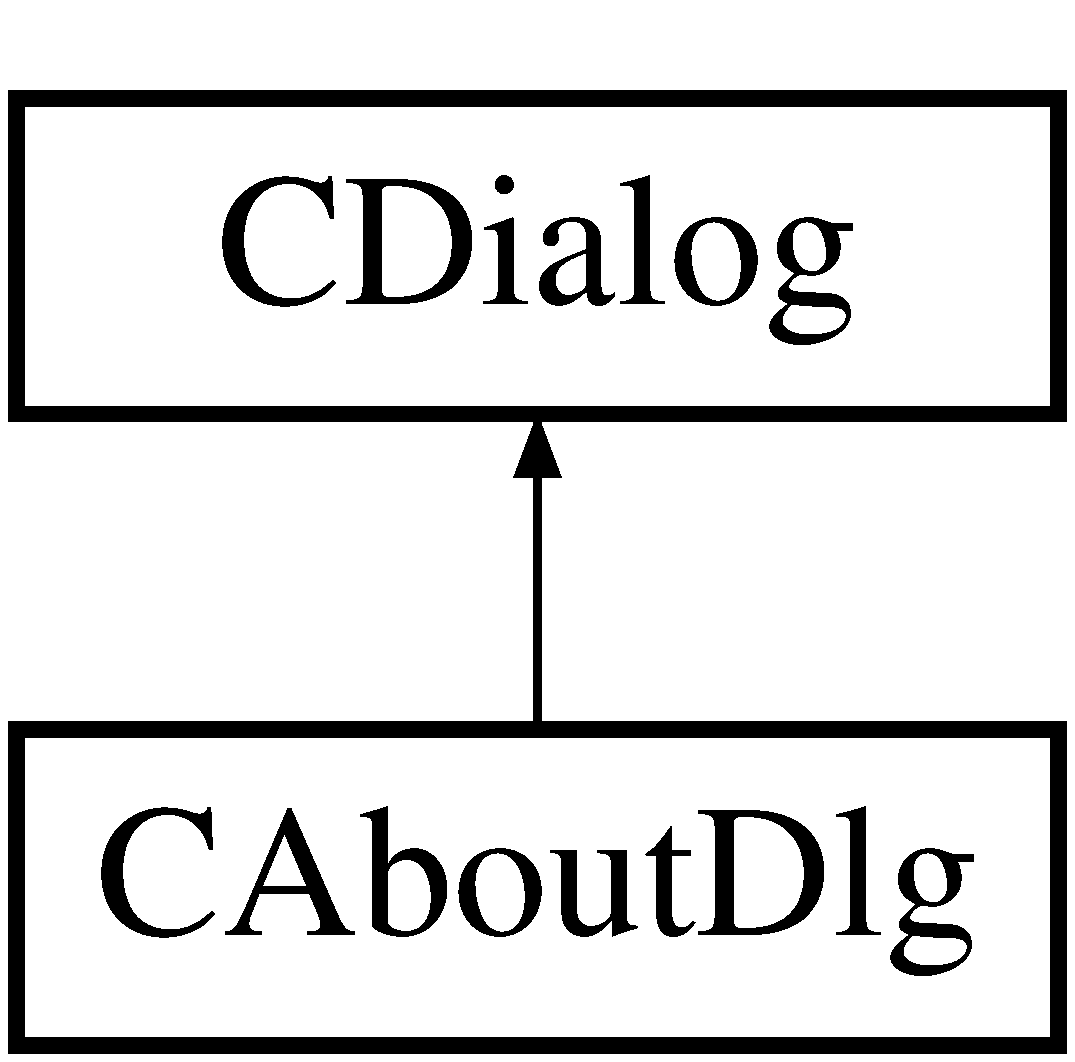
\includegraphics[height=2.000000cm]{class_c_about_dlg}
\end{center}
\end{figure}
\subsection*{Public Types}
\begin{DoxyCompactItemize}
\item 
\mbox{\Hypertarget{class_c_about_dlg_a68823db74a70b5e165bcd5e108852ce4}\label{class_c_about_dlg_a68823db74a70b5e165bcd5e108852ce4}} 
enum \{ {\bfseries I\+DD} = I\+D\+D\+\_\+\+A\+B\+O\+U\+T\+B\+OX
 \}
\end{DoxyCompactItemize}
\subsection*{Protected Member Functions}
\begin{DoxyCompactItemize}
\item 
\mbox{\Hypertarget{class_c_about_dlg_ab83db7484fec957282d7d5a21aed4df4}\label{class_c_about_dlg_ab83db7484fec957282d7d5a21aed4df4}} 
virtual void {\bfseries Do\+Data\+Exchange} (C\+Data\+Exchange $\ast$p\+DX)
\end{DoxyCompactItemize}


The documentation for this class was generated from the following file\+:\begin{DoxyCompactItemize}
\item 
i\+Optics/i\+Optics.\+cpp\end{DoxyCompactItemize}

\hypertarget{class_c_main_app}{}\section{C\+Main\+App Class Reference}
\label{class_c_main_app}\index{C\+Main\+App@{C\+Main\+App}}
Inheritance diagram for C\+Main\+App\+:\begin{figure}[H]
\begin{center}
\leavevmode
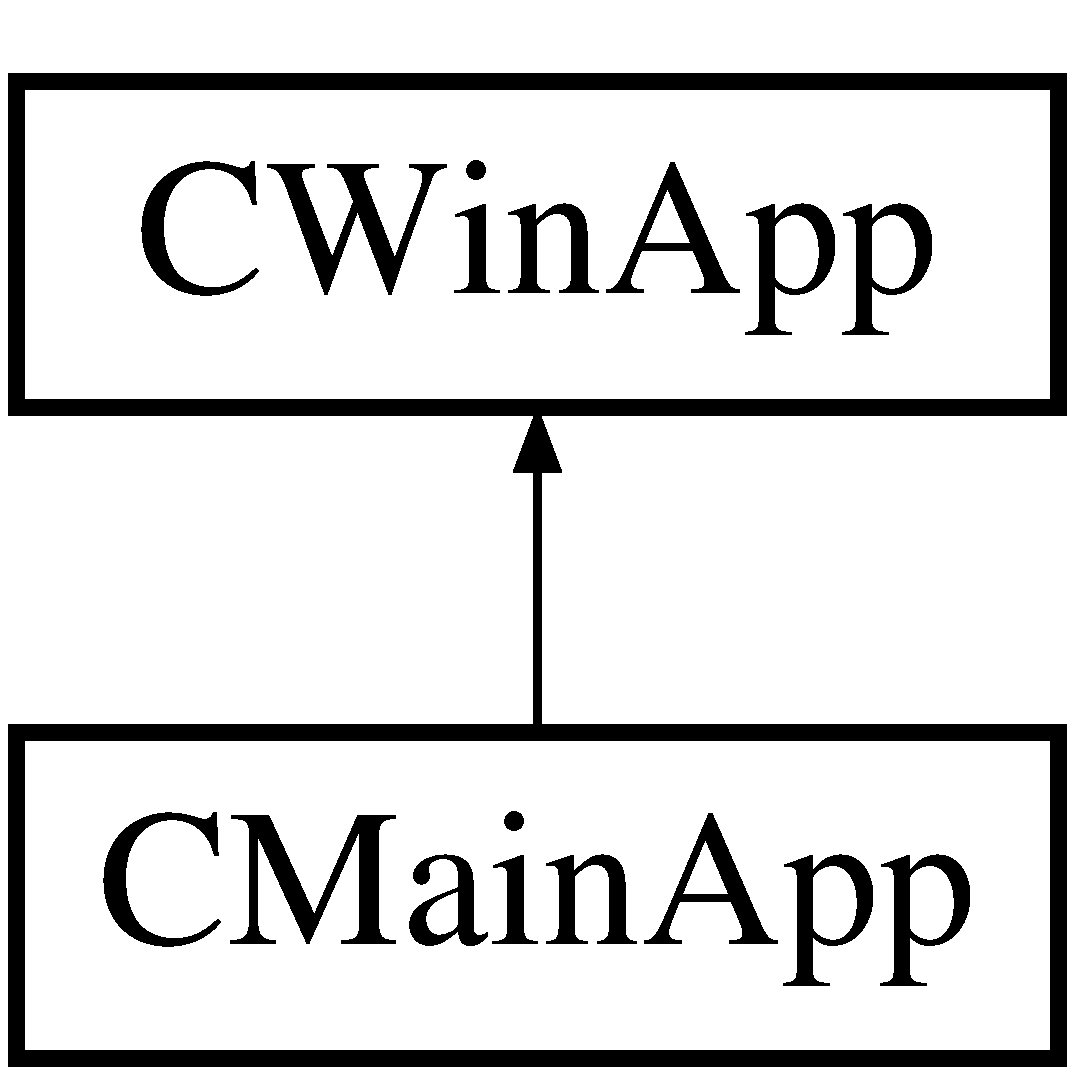
\includegraphics[height=2.000000cm]{class_c_main_app}
\end{center}
\end{figure}
\subsection*{Public Member Functions}
\begin{DoxyCompactItemize}
\item 
\mbox{\Hypertarget{class_c_main_app_a015a0ebfae1ea6e610095915d8976191}\label{class_c_main_app_a015a0ebfae1ea6e610095915d8976191}} 
virtual B\+O\+OL {\bfseries Init\+Instance} ()
\item 
\mbox{\Hypertarget{class_c_main_app_a508ce7ca12845b706e73fb65cf83329b}\label{class_c_main_app_a508ce7ca12845b706e73fb65cf83329b}} 
afx\+\_\+msg void {\bfseries On\+App\+About} ()
\end{DoxyCompactItemize}


The documentation for this class was generated from the following files\+:\begin{DoxyCompactItemize}
\item 
i\+Optics/i\+Optics.\+h\item 
i\+Optics/i\+Optics.\+cpp\end{DoxyCompactItemize}

\hypertarget{class_c_main_doc}{}\section{C\+Main\+Doc Class Reference}
\label{class_c_main_doc}\index{C\+Main\+Doc@{C\+Main\+Doc}}
Inheritance diagram for C\+Main\+Doc\+:\begin{figure}[H]
\begin{center}
\leavevmode
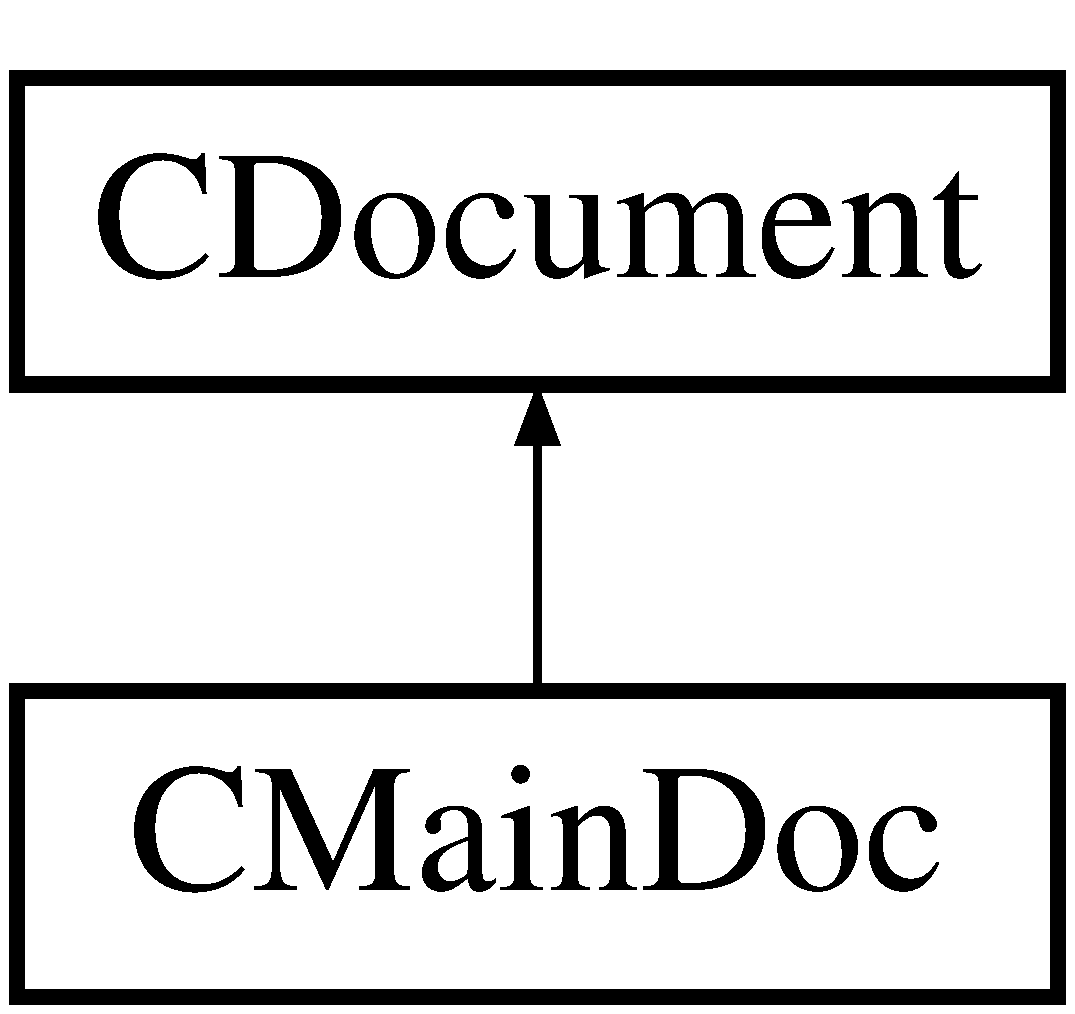
\includegraphics[height=2.000000cm]{class_c_main_doc}
\end{center}
\end{figure}
\subsection*{Public Member Functions}
\begin{DoxyCompactItemize}
\item 
\mbox{\Hypertarget{class_c_main_doc_a76e8b5aa95766a847bb11ac63e310dcc}\label{class_c_main_doc_a76e8b5aa95766a847bb11ac63e310dcc}} 
Img\+File $\ast$ {\bfseries Get\+Image} ()
\item 
\mbox{\Hypertarget{class_c_main_doc_ad1100572b5a4148e920b70268c37feb5}\label{class_c_main_doc_ad1100572b5a4148e920b70268c37feb5}} 
B\+O\+OL {\bfseries Update\+Image} (Img\+File $\ast$p\+Img)
\item 
\mbox{\Hypertarget{class_c_main_doc_aa9d7df83c9c244c5699f6432c5d621dc}\label{class_c_main_doc_aa9d7df83c9c244c5699f6432c5d621dc}} 
S\+I\+ZE {\bfseries Get\+Image\+Size} ()
\item 
\mbox{\Hypertarget{class_c_main_doc_a126f38d2277d2836557658480fd1871b}\label{class_c_main_doc_a126f38d2277d2836557658480fd1871b}} 
virtual B\+O\+OL {\bfseries On\+New\+Document} ()
\item 
\mbox{\Hypertarget{class_c_main_doc_a602c573ee0f41036fa81f45c4640ba94}\label{class_c_main_doc_a602c573ee0f41036fa81f45c4640ba94}} 
virtual void {\bfseries Serialize} (C\+Archive \&ar)
\item 
\mbox{\Hypertarget{class_c_main_doc_a0b20ba47b6491164edd00071d05ae0c2}\label{class_c_main_doc_a0b20ba47b6491164edd00071d05ae0c2}} 
virtual void {\bfseries Delete\+Contents} ()
\item 
\mbox{\Hypertarget{class_c_main_doc_af72ef9a0f0ea90f3447ad861cb3a34d4}\label{class_c_main_doc_af72ef9a0f0ea90f3447ad861cb3a34d4}} 
virtual B\+O\+OL {\bfseries On\+Open\+Document} (L\+P\+C\+T\+S\+TR lpsz\+Path\+Name)
\item 
\mbox{\Hypertarget{class_c_main_doc_ae2023d992f49d22b105fc52979074136}\label{class_c_main_doc_ae2023d992f49d22b105fc52979074136}} 
virtual B\+O\+OL {\bfseries On\+Save\+Document} (L\+P\+C\+T\+S\+TR lpsz\+Path\+Name)
\end{DoxyCompactItemize}
\subsection*{Protected Member Functions}
\begin{DoxyCompactItemize}
\item 
\mbox{\Hypertarget{class_c_main_doc_a8213ee6e6cc2362c108a23397deaea75}\label{class_c_main_doc_a8213ee6e6cc2362c108a23397deaea75}} 
afx\+\_\+msg void {\bfseries On\+File\+Save\+As} ()
\item 
\mbox{\Hypertarget{class_c_main_doc_afd3859fa6725882b108930ba060b1b52}\label{class_c_main_doc_afd3859fa6725882b108930ba060b1b52}} 
afx\+\_\+msg void {\bfseries On\+Update\+File\+Save\+As} (C\+Cmd\+UI $\ast$p\+Cmd\+UI)
\item 
\mbox{\Hypertarget{class_c_main_doc_a367feb33c52af2fba6684b052b5a5d37}\label{class_c_main_doc_a367feb33c52af2fba6684b052b5a5d37}} 
afx\+\_\+msg void {\bfseries On\+File\+Save} ()
\item 
\mbox{\Hypertarget{class_c_main_doc_a25b7cad95cf95daa5a9028ebcf323ddf}\label{class_c_main_doc_a25b7cad95cf95daa5a9028ebcf323ddf}} 
afx\+\_\+msg void {\bfseries On\+Update\+File\+Save} (C\+Cmd\+UI $\ast$p\+Cmd\+UI)
\end{DoxyCompactItemize}
\subsection*{Protected Attributes}
\begin{DoxyCompactItemize}
\item 
\mbox{\Hypertarget{class_c_main_doc_a5c68f04aec7608ec7be0443e244a2438}\label{class_c_main_doc_a5c68f04aec7608ec7be0443e244a2438}} 
Img\+File $\ast$ {\bfseries m\+\_\+p\+Img}
\item 
\mbox{\Hypertarget{class_c_main_doc_a2ed43e97d3248881e178d69647aebdde}\label{class_c_main_doc_a2ed43e97d3248881e178d69647aebdde}} 
Img\+File $\ast$ {\bfseries m\+\_\+p\+Img\+Edge}
\item 
\mbox{\Hypertarget{class_c_main_doc_a49074efdff7dc3cbdfd460bea387a05b}\label{class_c_main_doc_a49074efdff7dc3cbdfd460bea387a05b}} 
Img\+File $\ast$ {\bfseries m\+\_\+p\+Img\+Out}
\item 
\mbox{\Hypertarget{class_c_main_doc_a194f4b9748851f84b9cd018f3aa9a363}\label{class_c_main_doc_a194f4b9748851f84b9cd018f3aa9a363}} 
S\+I\+ZE {\bfseries m\+\_\+sz\+Image}
\end{DoxyCompactItemize}


The documentation for this class was generated from the following files\+:\begin{DoxyCompactItemize}
\item 
i\+Optics/Main\+Doc.\+h\item 
i\+Optics/Main\+Doc.\+cpp\end{DoxyCompactItemize}

\hypertarget{class_c_main_frame}{}\section{C\+Main\+Frame Class Reference}
\label{class_c_main_frame}\index{C\+Main\+Frame@{C\+Main\+Frame}}
Inheritance diagram for C\+Main\+Frame\+:\begin{figure}[H]
\begin{center}
\leavevmode
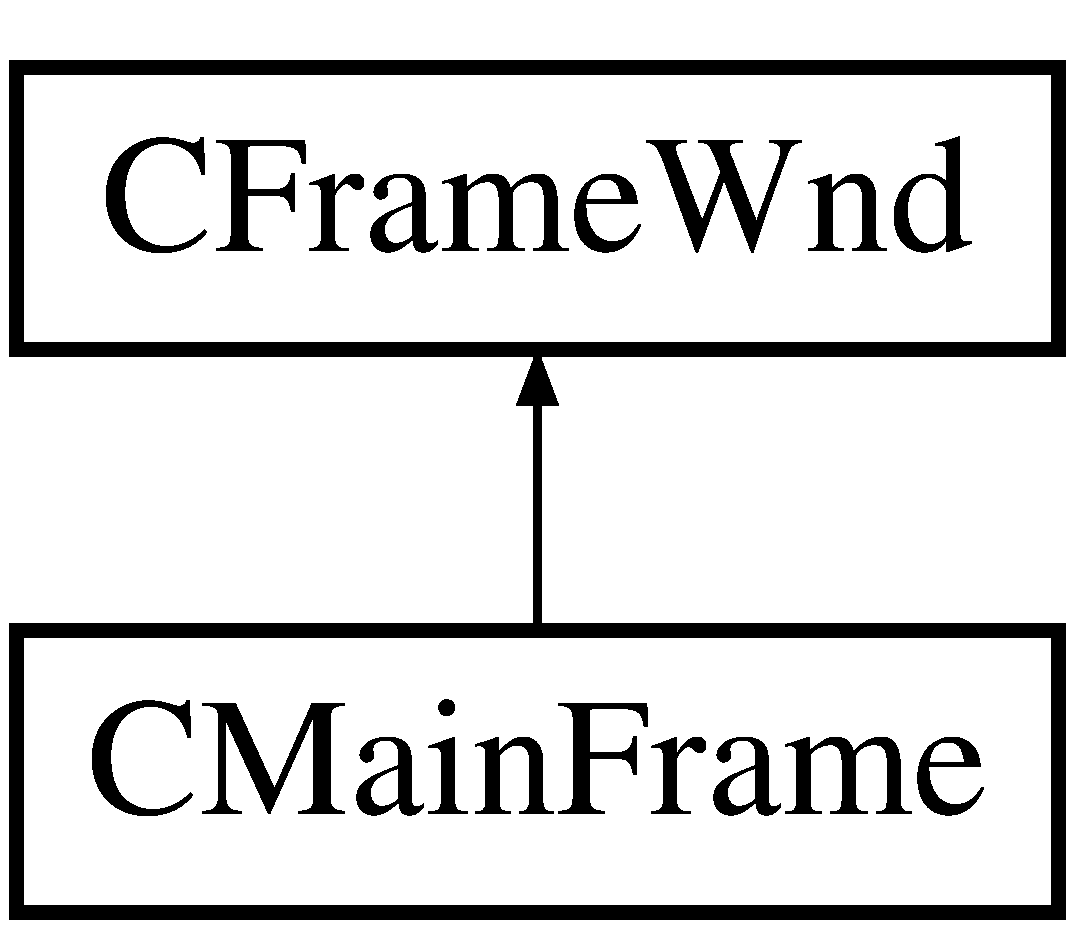
\includegraphics[height=2.000000cm]{class_c_main_frame}
\end{center}
\end{figure}
\subsection*{Public Member Functions}
\begin{DoxyCompactItemize}
\item 
\mbox{\Hypertarget{class_c_main_frame_a549bf677c955c2898c3c683321633c16}\label{class_c_main_frame_a549bf677c955c2898c3c683321633c16}} 
virtual B\+O\+OL {\bfseries Pre\+Create\+Window} (C\+R\+E\+A\+T\+E\+S\+T\+R\+U\+CT \&cs)
\end{DoxyCompactItemize}
\subsection*{Protected Member Functions}
\begin{DoxyCompactItemize}
\item 
\mbox{\Hypertarget{class_c_main_frame_ad5edd671a359b7958eaf78916fa69a42}\label{class_c_main_frame_ad5edd671a359b7958eaf78916fa69a42}} 
B\+O\+OL {\bfseries Create\+Tool\+Bar} ()
\item 
\mbox{\Hypertarget{class_c_main_frame_a31e574e7c7f60aa3fea901c8f81e69ec}\label{class_c_main_frame_a31e574e7c7f60aa3fea901c8f81e69ec}} 
B\+O\+OL {\bfseries Create\+Palette\+Bar} ()
\item 
\mbox{\Hypertarget{class_c_main_frame_a48666466fd37412fcaeff75c3b12e0ed}\label{class_c_main_frame_a48666466fd37412fcaeff75c3b12e0ed}} 
afx\+\_\+msg int {\bfseries On\+Create} (L\+P\+C\+R\+E\+A\+T\+E\+S\+T\+R\+U\+CT lp\+Create\+Struct)
\item 
\mbox{\Hypertarget{class_c_main_frame_acc76d5562454352a0e51c0894c1dfa07}\label{class_c_main_frame_acc76d5562454352a0e51c0894c1dfa07}} 
afx\+\_\+msg void {\bfseries On\+View\+Short} ()
\end{DoxyCompactItemize}
\subsection*{Protected Attributes}
\begin{DoxyCompactItemize}
\item 
\mbox{\Hypertarget{class_c_main_frame_ac01bafc03aee69cf982e6f029b4db6b0}\label{class_c_main_frame_ac01bafc03aee69cf982e6f029b4db6b0}} 
C\+Status\+Bar {\bfseries m\+\_\+wnd\+Status\+Bar}
\item 
\mbox{\Hypertarget{class_c_main_frame_a73024d794dce2fe918f6b117371c25fc}\label{class_c_main_frame_a73024d794dce2fe918f6b117371c25fc}} 
C\+Tool\+Bar {\bfseries m\+\_\+wnd\+Tool\+Bar}
\item 
\mbox{\Hypertarget{class_c_main_frame_aa9c4f31a06e06b7f0ee53b21b449a5d3}\label{class_c_main_frame_aa9c4f31a06e06b7f0ee53b21b449a5d3}} 
\mbox{\hyperlink{class_c_palette_bar}{C\+Palette\+Bar}} {\bfseries m\+\_\+wnd\+Tool\+Box}
\end{DoxyCompactItemize}


The documentation for this class was generated from the following files\+:\begin{DoxyCompactItemize}
\item 
i\+Optics/Main\+Frm.\+h\item 
i\+Optics/Main\+Frm.\+cpp\end{DoxyCompactItemize}

\hypertarget{class_c_main_view}{}\section{C\+Main\+View Class Reference}
\label{class_c_main_view}\index{C\+Main\+View@{C\+Main\+View}}
Inheritance diagram for C\+Main\+View\+:\begin{figure}[H]
\begin{center}
\leavevmode
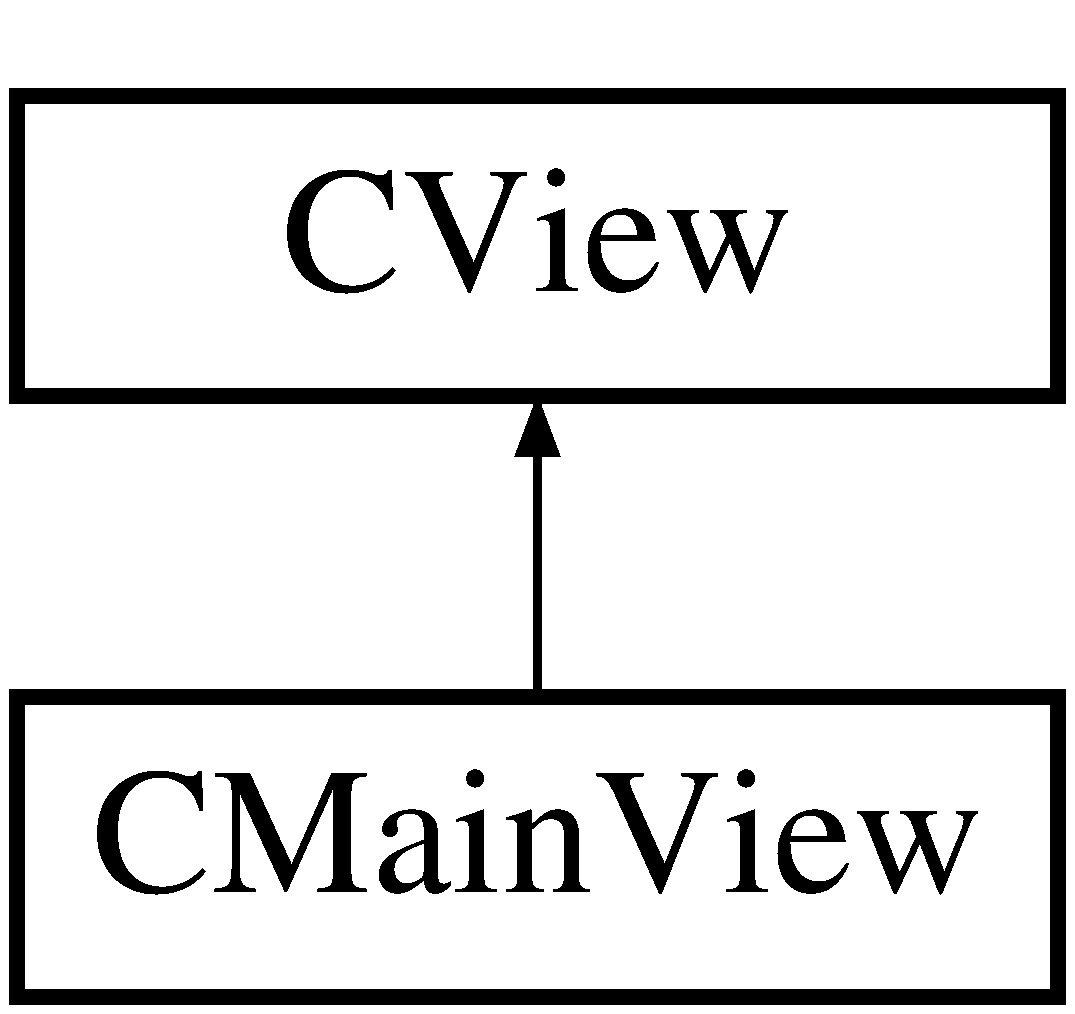
\includegraphics[height=2.000000cm]{class_c_main_view}
\end{center}
\end{figure}
\subsection*{Public Member Functions}
\begin{DoxyCompactItemize}
\item 
\mbox{\Hypertarget{class_c_main_view_a5bf6e026f365e546ca8374b5abd645ad}\label{class_c_main_view_a5bf6e026f365e546ca8374b5abd645ad}} 
void {\bfseries Update\+Scroll\+Bar} (int n\+Bar, int pos, int page, int range)
\item 
\mbox{\Hypertarget{class_c_main_view_a83cc03d948f6cc6c340d54bcb7b7e82f}\label{class_c_main_view_a83cc03d948f6cc6c340d54bcb7b7e82f}} 
\mbox{\hyperlink{class_c_main_doc}{C\+Main\+Doc}} $\ast$ {\bfseries Get\+Document} ()
\item 
\mbox{\Hypertarget{class_c_main_view_ab6591df421b218553f828f82510bf894}\label{class_c_main_view_ab6591df421b218553f828f82510bf894}} 
Img\+File $\ast$ {\bfseries Get\+Img\+File} ()
\item 
\mbox{\Hypertarget{class_c_main_view_aa0751b941709df63bddf26f5db864fc6}\label{class_c_main_view_aa0751b941709df63bddf26f5db864fc6}} 
virtual B\+O\+OL {\bfseries On\+Cmd\+Msg} (U\+I\+NT n\+ID, int n\+Code, void $\ast$p\+Extra, A\+F\+X\+\_\+\+C\+M\+D\+H\+A\+N\+D\+L\+E\+R\+I\+N\+FO $\ast$p\+Handler\+Info)
\item 
\mbox{\Hypertarget{class_c_main_view_a4f5be0f4b4dc0f6a763235a945f235b8}\label{class_c_main_view_a4f5be0f4b4dc0f6a763235a945f235b8}} 
virtual void {\bfseries On\+Draw} (C\+DC $\ast$p\+DC)
\item 
\mbox{\Hypertarget{class_c_main_view_a1d20bfde9a44e6276224976590265145}\label{class_c_main_view_a1d20bfde9a44e6276224976590265145}} 
virtual B\+O\+OL {\bfseries Pre\+Create\+Window} (C\+R\+E\+A\+T\+E\+S\+T\+R\+U\+CT \&cs)
\item 
\mbox{\Hypertarget{class_c_main_view_a6f7ba208c41d8e0e1ad4f3796713b0b4}\label{class_c_main_view_a6f7ba208c41d8e0e1ad4f3796713b0b4}} 
afx\+\_\+msg int {\bfseries On\+Create} (L\+P\+C\+R\+E\+A\+T\+E\+S\+T\+R\+U\+CT lp\+Create\+Struct)
\item 
\mbox{\Hypertarget{class_c_main_view_ab4cedd67cf9ccc27d1377da0d3ba74e3}\label{class_c_main_view_ab4cedd67cf9ccc27d1377da0d3ba74e3}} 
afx\+\_\+msg void {\bfseries On\+Set\+Focus} (C\+Wnd $\ast$p\+Old\+Wnd)
\item 
\mbox{\Hypertarget{class_c_main_view_a3aef8932f9fb39a00389267d964b9035}\label{class_c_main_view_a3aef8932f9fb39a00389267d964b9035}} 
afx\+\_\+msg void {\bfseries On\+View\+Ruler} ()
\item 
\mbox{\Hypertarget{class_c_main_view_a3746d556ae77e54015535bd070b248a6}\label{class_c_main_view_a3746d556ae77e54015535bd070b248a6}} 
afx\+\_\+msg void {\bfseries On\+Update\+View\+Ruler} (C\+Cmd\+UI $\ast$p\+Cmd\+UI)
\item 
\mbox{\Hypertarget{class_c_main_view_a0cba96698760791da1ddd9f78f0d78eb}\label{class_c_main_view_a0cba96698760791da1ddd9f78f0d78eb}} 
afx\+\_\+msg void {\bfseries On\+Indicate\+Size} ()
\item 
\mbox{\Hypertarget{class_c_main_view_abe25a8c945ca92c6f6df3d5e2649c1f3}\label{class_c_main_view_abe25a8c945ca92c6f6df3d5e2649c1f3}} 
afx\+\_\+msg void {\bfseries On\+Update\+Indicate\+Size} (C\+Cmd\+UI $\ast$p\+Cmd\+UI)
\end{DoxyCompactItemize}
\subsection*{Public Attributes}
\begin{DoxyCompactItemize}
\item 
\mbox{\Hypertarget{class_c_main_view_a563cc9c66c8a922fecafada5c2cc2d6f}\label{class_c_main_view_a563cc9c66c8a922fecafada5c2cc2d6f}} 
\mbox{\hyperlink{class_navigator}{Navigator}} $\ast$ {\bfseries m\+\_\+p\+Navigator}
\end{DoxyCompactItemize}
\subsection*{Protected Member Functions}
\begin{DoxyCompactItemize}
\item 
\mbox{\Hypertarget{class_c_main_view_a93bdba23fa8dba336cd7db35eb969a95}\label{class_c_main_view_a93bdba23fa8dba336cd7db35eb969a95}} 
virtual void {\bfseries On\+Initial\+Update} ()
\item 
\mbox{\Hypertarget{class_c_main_view_a31c5f6d53bc32a681bc3734b80bbf8e8}\label{class_c_main_view_a31c5f6d53bc32a681bc3734b80bbf8e8}} 
virtual void {\bfseries On\+Update} (C\+View $\ast$p\+Sender, L\+P\+A\+R\+AM l\+Hint, C\+Object $\ast$p\+Hint)
\item 
\mbox{\Hypertarget{class_c_main_view_ad124fdedf5446133d7f0bd8215dab7f3}\label{class_c_main_view_ad124fdedf5446133d7f0bd8215dab7f3}} 
afx\+\_\+msg void {\bfseries On\+H\+Scroll} (U\+I\+NT n\+S\+B\+Code, U\+I\+NT n\+Pos, C\+Scroll\+Bar $\ast$p\+Scroll\+Bar)
\item 
\mbox{\Hypertarget{class_c_main_view_a4aac5578dc8d6b4675dcf328e0c733a8}\label{class_c_main_view_a4aac5578dc8d6b4675dcf328e0c733a8}} 
afx\+\_\+msg void {\bfseries On\+V\+Scroll} (U\+I\+NT n\+S\+B\+Code, U\+I\+NT n\+Pos, C\+Scroll\+Bar $\ast$p\+Scroll\+Bar)
\item 
\mbox{\Hypertarget{class_c_main_view_ac2b15b975f167969c9903f7264565607}\label{class_c_main_view_ac2b15b975f167969c9903f7264565607}} 
afx\+\_\+msg void {\bfseries On\+Size} (U\+I\+NT n\+Type, int cx, int cy)
\item 
\mbox{\Hypertarget{class_c_main_view_a1c9c04a4992fa275696d7a58e927c2be}\label{class_c_main_view_a1c9c04a4992fa275696d7a58e927c2be}} 
afx\+\_\+msg void {\bfseries On\+V\+I\+E\+W\+Navigater} ()
\item 
\mbox{\Hypertarget{class_c_main_view_a9df07ffc397963f1347b952d0fcfb9ea}\label{class_c_main_view_a9df07ffc397963f1347b952d0fcfb9ea}} 
afx\+\_\+msg void {\bfseries On\+Update\+V\+I\+E\+W\+Navigater} (C\+Cmd\+UI $\ast$p\+Cmd\+UI)
\end{DoxyCompactItemize}


The documentation for this class was generated from the following files\+:\begin{DoxyCompactItemize}
\item 
i\+Optics/Main\+View.\+h\item 
i\+Optics/Main\+View.\+cpp\end{DoxyCompactItemize}

\hypertarget{class_c_palette_bar}{}\section{C\+Palette\+Bar Class Reference}
\label{class_c_palette_bar}\index{C\+Palette\+Bar@{C\+Palette\+Bar}}
Inheritance diagram for C\+Palette\+Bar\+:\begin{figure}[H]
\begin{center}
\leavevmode
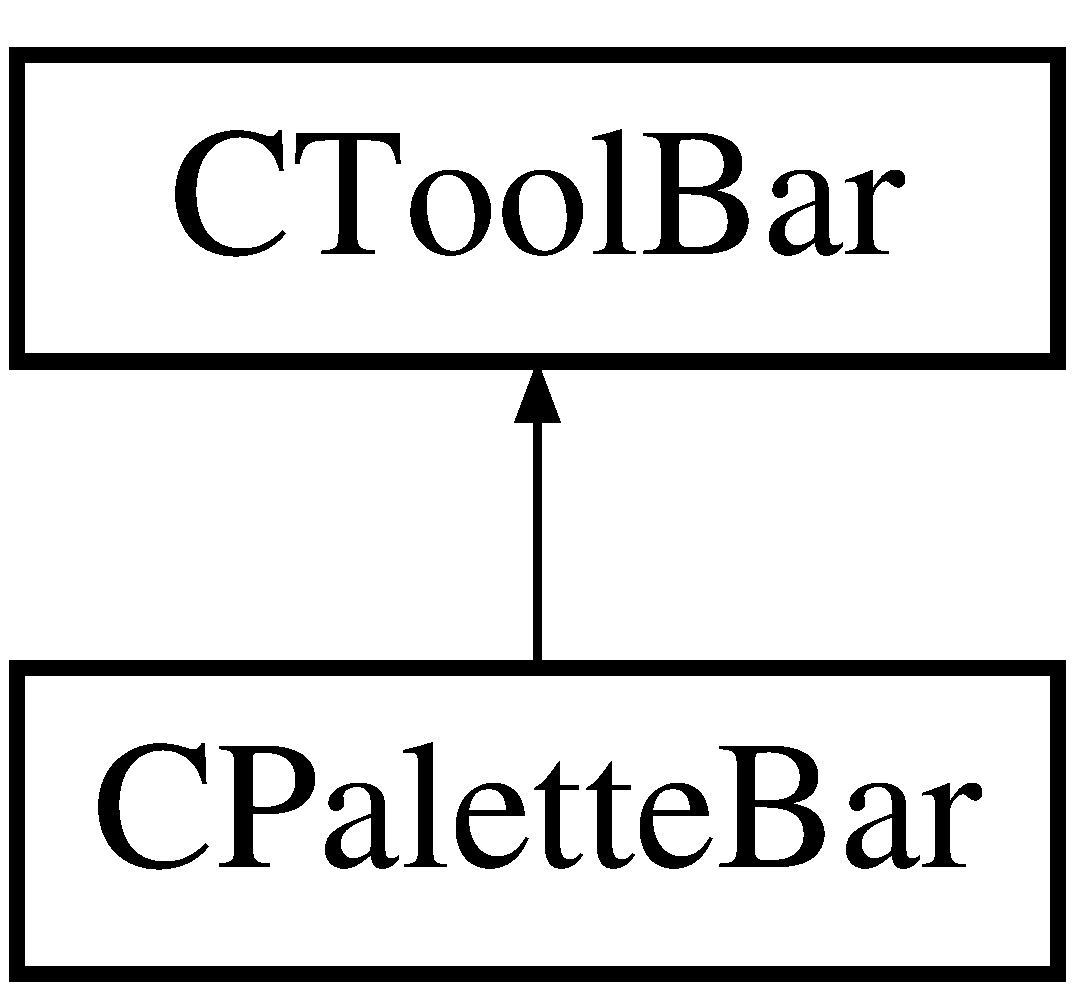
\includegraphics[height=2.000000cm]{class_c_palette_bar}
\end{center}
\end{figure}
\subsection*{Public Member Functions}
\begin{DoxyCompactItemize}
\item 
\mbox{\Hypertarget{class_c_palette_bar_aaf4c9748f0ed14e27c7d297501b58a6e}\label{class_c_palette_bar_aaf4c9748f0ed14e27c7d297501b58a6e}} 
void {\bfseries Set\+Columns} (U\+I\+NT n\+Columns)
\item 
\mbox{\Hypertarget{class_c_palette_bar_a3640a2a9326b4924506593412c2e4dad}\label{class_c_palette_bar_a3640a2a9326b4924506593412c2e4dad}} 
U\+I\+NT {\bfseries Get\+Columns} ()
\end{DoxyCompactItemize}
\subsection*{Protected Attributes}
\begin{DoxyCompactItemize}
\item 
\mbox{\Hypertarget{class_c_palette_bar_a1e1370ae0bdfb486d4a2284023f27d03}\label{class_c_palette_bar_a1e1370ae0bdfb486d4a2284023f27d03}} 
U\+I\+NT {\bfseries m\+\_\+n\+Columns}
\end{DoxyCompactItemize}


The documentation for this class was generated from the following files\+:\begin{DoxyCompactItemize}
\item 
i\+Optics/palette.\+h\item 
i\+Optics/palette.\+cpp\end{DoxyCompactItemize}

\hypertarget{class_c_ruler_corner_view}{}\section{C\+Ruler\+Corner\+View Class Reference}
\label{class_c_ruler_corner_view}\index{C\+Ruler\+Corner\+View@{C\+Ruler\+Corner\+View}}
Inheritance diagram for C\+Ruler\+Corner\+View\+:\begin{figure}[H]
\begin{center}
\leavevmode
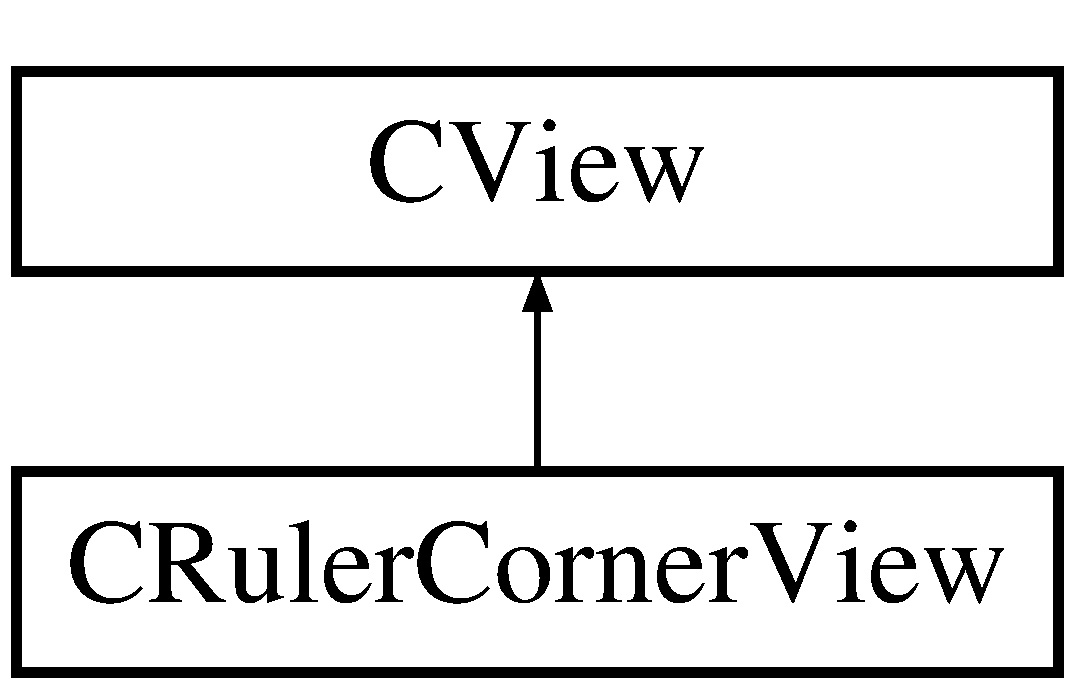
\includegraphics[height=2.000000cm]{class_c_ruler_corner_view}
\end{center}
\end{figure}
\subsection*{Protected Member Functions}
\begin{DoxyCompactItemize}
\item 
\mbox{\Hypertarget{class_c_ruler_corner_view_a8ce27cc078fe4056f1f4f0fdbe6c0c66}\label{class_c_ruler_corner_view_a8ce27cc078fe4056f1f4f0fdbe6c0c66}} 
virtual void {\bfseries On\+Draw} (C\+DC $\ast$p\+DC)
\item 
\mbox{\Hypertarget{class_c_ruler_corner_view_a204e8f055a1e067b8df69ae8c758954f}\label{class_c_ruler_corner_view_a204e8f055a1e067b8df69ae8c758954f}} 
virtual B\+O\+OL {\bfseries Pre\+Create\+Window} (C\+R\+E\+A\+T\+E\+S\+T\+R\+U\+CT \&cs)
\end{DoxyCompactItemize}


The documentation for this class was generated from the following file\+:\begin{DoxyCompactItemize}
\item 
i\+Optics/ruler.\+h\end{DoxyCompactItemize}

\hypertarget{class_c_ruler_splitter_wnd}{}\section{C\+Ruler\+Splitter\+Wnd Class Reference}
\label{class_c_ruler_splitter_wnd}\index{C\+Ruler\+Splitter\+Wnd@{C\+Ruler\+Splitter\+Wnd}}
Inheritance diagram for C\+Ruler\+Splitter\+Wnd\+:\begin{figure}[H]
\begin{center}
\leavevmode
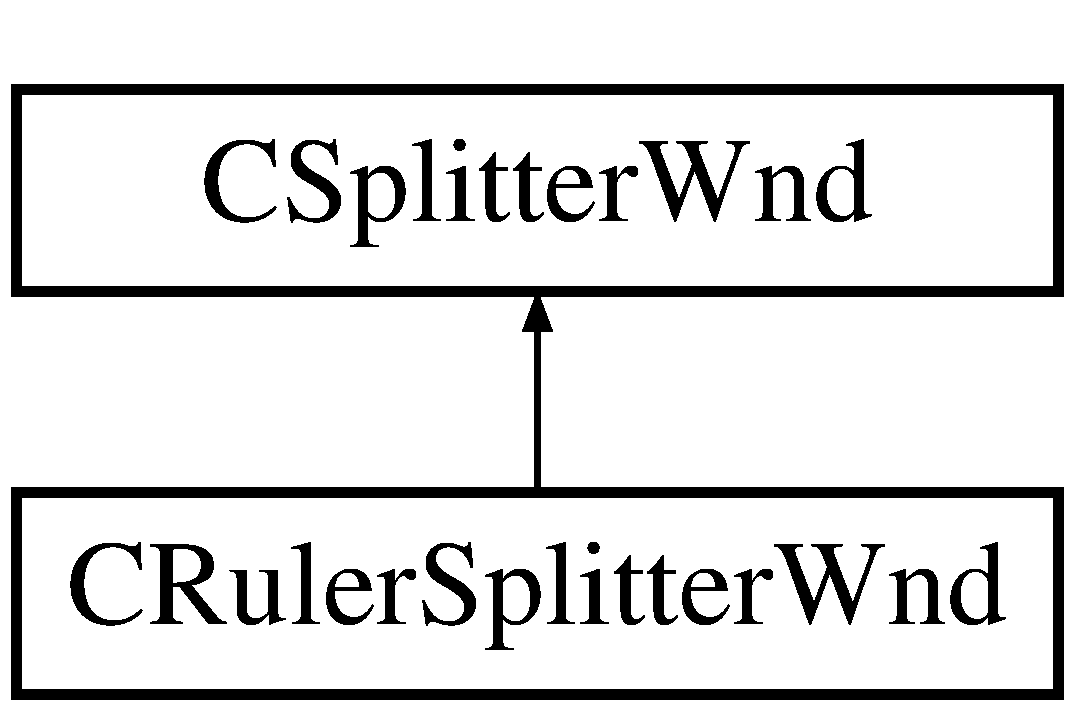
\includegraphics[height=2.000000cm]{class_c_ruler_splitter_wnd}
\end{center}
\end{figure}
\subsection*{Public Member Functions}
\begin{DoxyCompactItemize}
\item 
\mbox{\Hypertarget{class_c_ruler_splitter_wnd_a7caada869d685266a750c022e6e260ec}\label{class_c_ruler_splitter_wnd_a7caada869d685266a750c022e6e260ec}} 
int {\bfseries Hit\+Test} (C\+Point pt) const
\end{DoxyCompactItemize}


The documentation for this class was generated from the following file\+:\begin{DoxyCompactItemize}
\item 
i\+Optics/ruler.\+h\end{DoxyCompactItemize}

\hypertarget{class_c_ruler_view}{}\section{C\+Ruler\+View Class Reference}
\label{class_c_ruler_view}\index{C\+Ruler\+View@{C\+Ruler\+View}}
Inheritance diagram for C\+Ruler\+View\+:\begin{figure}[H]
\begin{center}
\leavevmode
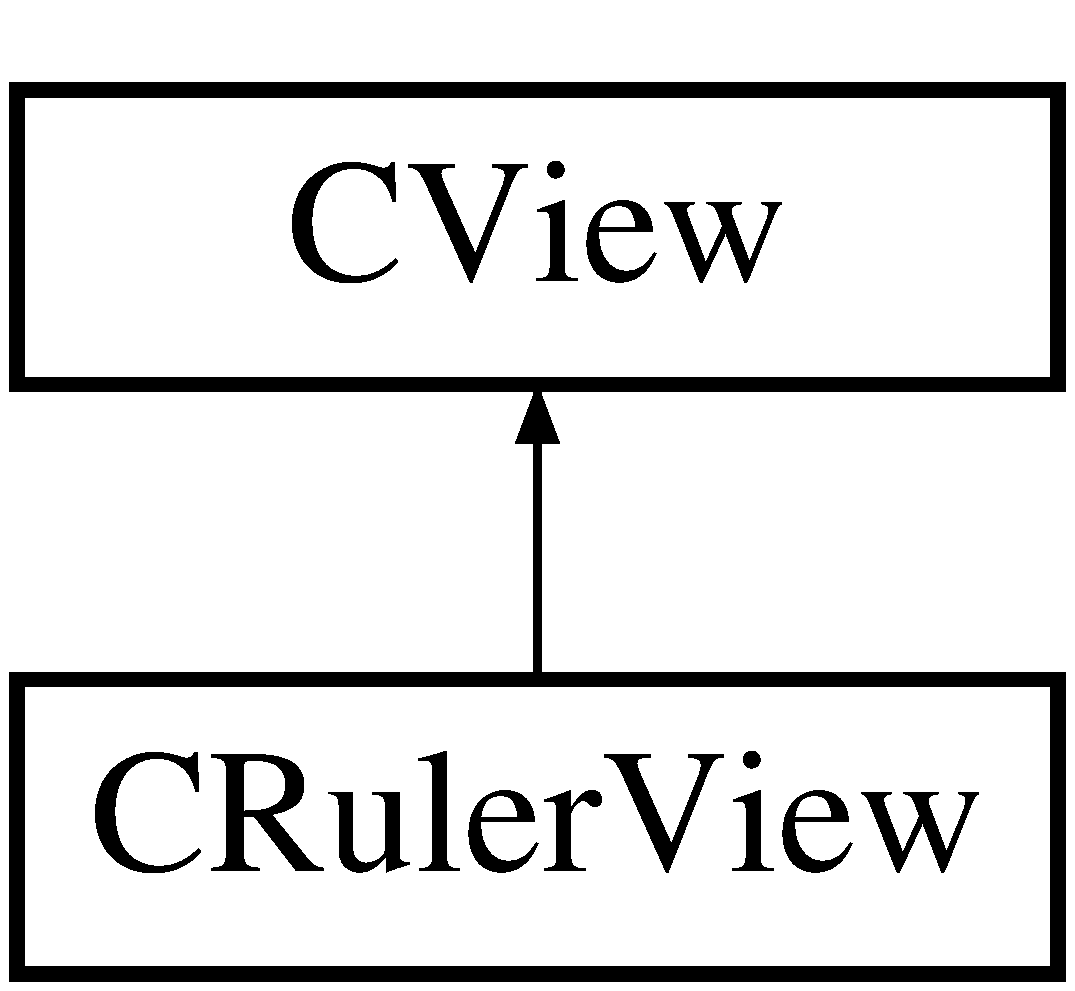
\includegraphics[height=2.000000cm]{class_c_ruler_view}
\end{center}
\end{figure}
\subsection*{Public Member Functions}
\begin{DoxyCompactItemize}
\item 
\mbox{\Hypertarget{class_c_ruler_view_af70f2eb8f5d2a49d532134be766cf1f2}\label{class_c_ruler_view_af70f2eb8f5d2a49d532134be766cf1f2}} 
C\+Some\+Doc $\ast$ {\bfseries Get\+Document} ()
\item 
\mbox{\Hypertarget{class_c_ruler_view_a5d8a04d5c63c4ed954a18fd05a3dd657}\label{class_c_ruler_view_a5d8a04d5c63c4ed954a18fd05a3dd657}} 
void {\bfseries Set\+Ruler\+Type} (U\+I\+NT ruler\+Type=R\+T\+\_\+\+H\+O\+R\+I\+Z\+O\+N\+T\+AL)
\item 
\mbox{\Hypertarget{class_c_ruler_view_a2a6c8504dea0b0df91704ff8acfdaf89}\label{class_c_ruler_view_a2a6c8504dea0b0df91704ff8acfdaf89}} 
virtual void {\bfseries On\+Initial\+Update} ()
\end{DoxyCompactItemize}
\subsection*{Public Attributes}
\begin{DoxyCompactItemize}
\item 
\mbox{\Hypertarget{class_c_ruler_view_a32f2c11d8836a3b2464600ff3c9e5001}\label{class_c_ruler_view_a32f2c11d8836a3b2464600ff3c9e5001}} 
U\+I\+NT {\bfseries m\+\_\+ruler\+Type}
\item 
\mbox{\Hypertarget{class_c_ruler_view_a29849fb8eb39e0b97e5fbdf61c49145c}\label{class_c_ruler_view_a29849fb8eb39e0b97e5fbdf61c49145c}} 
int {\bfseries m\+\_\+scroll\+Pos}
\end{DoxyCompactItemize}
\subsection*{Protected Member Functions}
\begin{DoxyCompactItemize}
\item 
\mbox{\Hypertarget{class_c_ruler_view_a69be569b6ac91a18a4f70110b88ec4fe}\label{class_c_ruler_view_a69be569b6ac91a18a4f70110b88ec4fe}} 
virtual void {\bfseries On\+Draw} (C\+DC $\ast$p\+DC)
\item 
\mbox{\Hypertarget{class_c_ruler_view_ae7699c2bc9045142feb92e885c8ca314}\label{class_c_ruler_view_ae7699c2bc9045142feb92e885c8ca314}} 
virtual B\+O\+OL {\bfseries Pre\+Create\+Window} (C\+R\+E\+A\+T\+E\+S\+T\+R\+U\+CT \&cs)
\item 
\mbox{\Hypertarget{class_c_ruler_view_a00f7c68e8e360ba6a9330af65c0ca4cf}\label{class_c_ruler_view_a00f7c68e8e360ba6a9330af65c0ca4cf}} 
virtual void {\bfseries On\+Update} (C\+View $\ast$p\+Sender, L\+P\+A\+R\+AM l\+Hint, C\+Object $\ast$p\+Hint)
\end{DoxyCompactItemize}
\subsection*{Protected Attributes}
\begin{DoxyCompactItemize}
\item 
\mbox{\Hypertarget{class_c_ruler_view_a9a6e088945b06267a191c9d8dd7f6916}\label{class_c_ruler_view_a9a6e088945b06267a191c9d8dd7f6916}} 
int {\bfseries m\+\_\+last\+Pos}
\end{DoxyCompactItemize}


The documentation for this class was generated from the following file\+:\begin{DoxyCompactItemize}
\item 
i\+Optics/ruler.\+h\end{DoxyCompactItemize}

\hypertarget{class_fec_gride}{}\section{Fec\+Gride Class Reference}
\label{class_fec_gride}\index{Fec\+Gride@{Fec\+Gride}}
Inheritance diagram for Fec\+Gride\+:\begin{figure}[H]
\begin{center}
\leavevmode
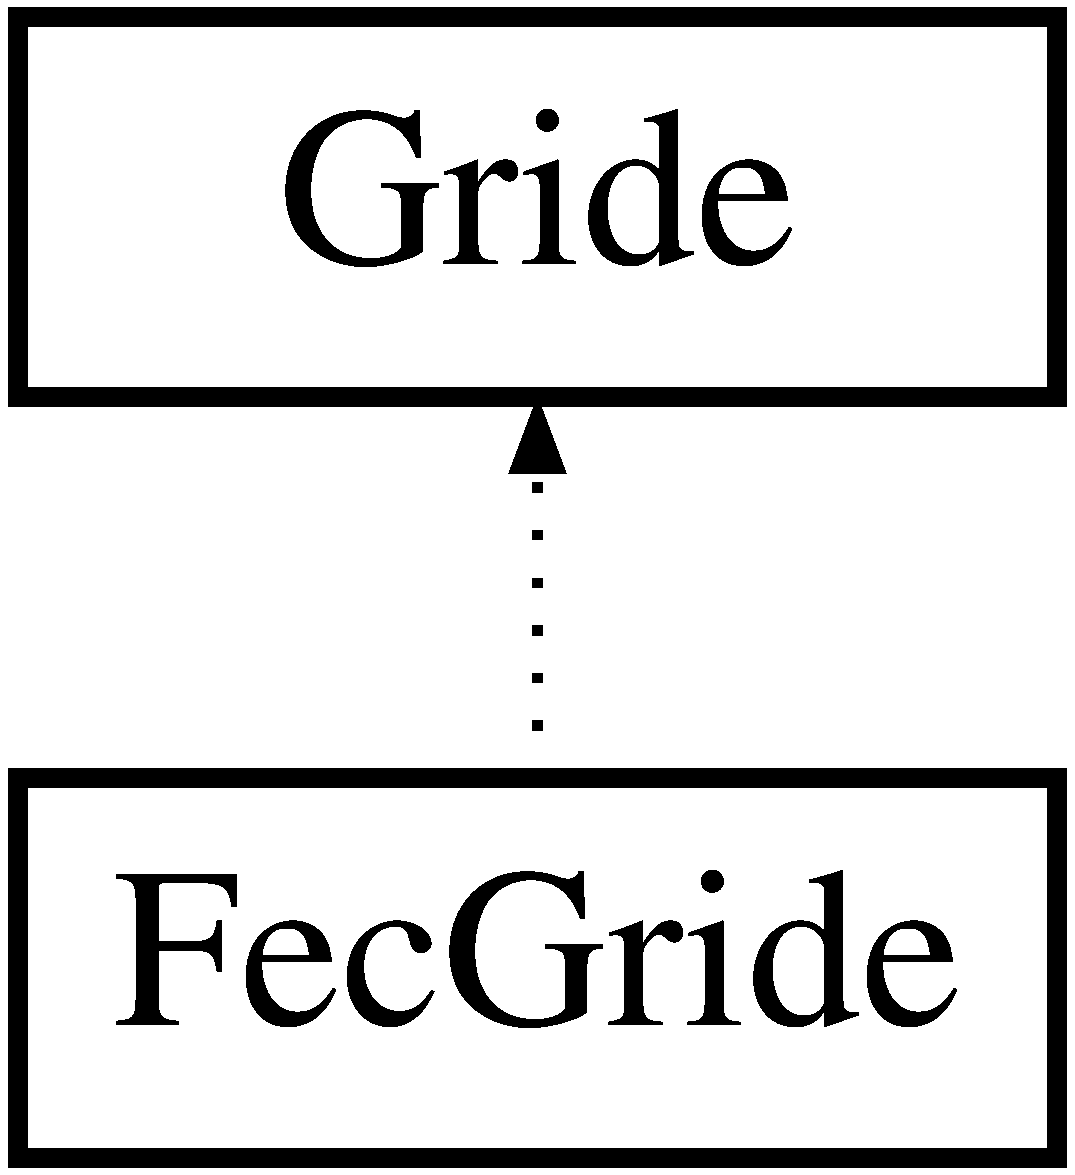
\includegraphics[height=2.000000cm]{class_fec_gride}
\end{center}
\end{figure}
\subsection*{Public Member Functions}
\begin{DoxyCompactItemize}
\item 
\mbox{\Hypertarget{class_fec_gride_ae079599de4464cc0323d2f576a5a3208}\label{class_fec_gride_ae079599de4464cc0323d2f576a5a3208}} 
{\bfseries Fec\+Gride} (C\+O\+L\+O\+R\+R\+EF color)
\item 
\mbox{\Hypertarget{class_fec_gride_a8b2a5b5290dfd68fce0ca3ed892e2609}\label{class_fec_gride_a8b2a5b5290dfd68fce0ca3ed892e2609}} 
virtual void {\bfseries Draw} (C\+DC $\ast$p\+DC)
\item 
\mbox{\Hypertarget{class_fec_gride_aec4499968594ccaf0531746926b562da}\label{class_fec_gride_aec4499968594ccaf0531746926b562da}} 
virtual void {\bfseries Set\+Param} (void $\ast$p\+Param)
\end{DoxyCompactItemize}
\subsection*{Protected Attributes}
\begin{DoxyCompactItemize}
\item 
\mbox{\Hypertarget{class_fec_gride_ad3ea90bbaa1bd84b5ed69b2c10232aad}\label{class_fec_gride_ad3ea90bbaa1bd84b5ed69b2c10232aad}} 
\mbox{\hyperlink{struct___fec_param}{Fec\+Param}} {\bfseries m\+\_\+param}
\end{DoxyCompactItemize}


The documentation for this class was generated from the following files\+:\begin{DoxyCompactItemize}
\item 
i\+Optics/Gride.\+h\item 
i\+Optics/Gride.\+cpp\end{DoxyCompactItemize}

\hypertarget{class_fec_tool}{}\section{Fec\+Tool Class Reference}
\label{class_fec_tool}\index{Fec\+Tool@{Fec\+Tool}}


\mbox{\hyperlink{class_fec_tool}{Fec\+Tool}} is used to control the settings of F\+EC process with UI in a dialog box. This class sends the parameters to a \mbox{\hyperlink{class_fec_view}{Fec\+View}} to display the resulted image. It also connects to a \mbox{\hyperlink{class_fec_wrap}{Fec\+Wrap}} class to maintain the F\+EC process related parameters and L\+UT data.  




{\ttfamily \#include $<$Fec\+Tool.\+h$>$}

Inheritance diagram for Fec\+Tool\+:\begin{figure}[H]
\begin{center}
\leavevmode
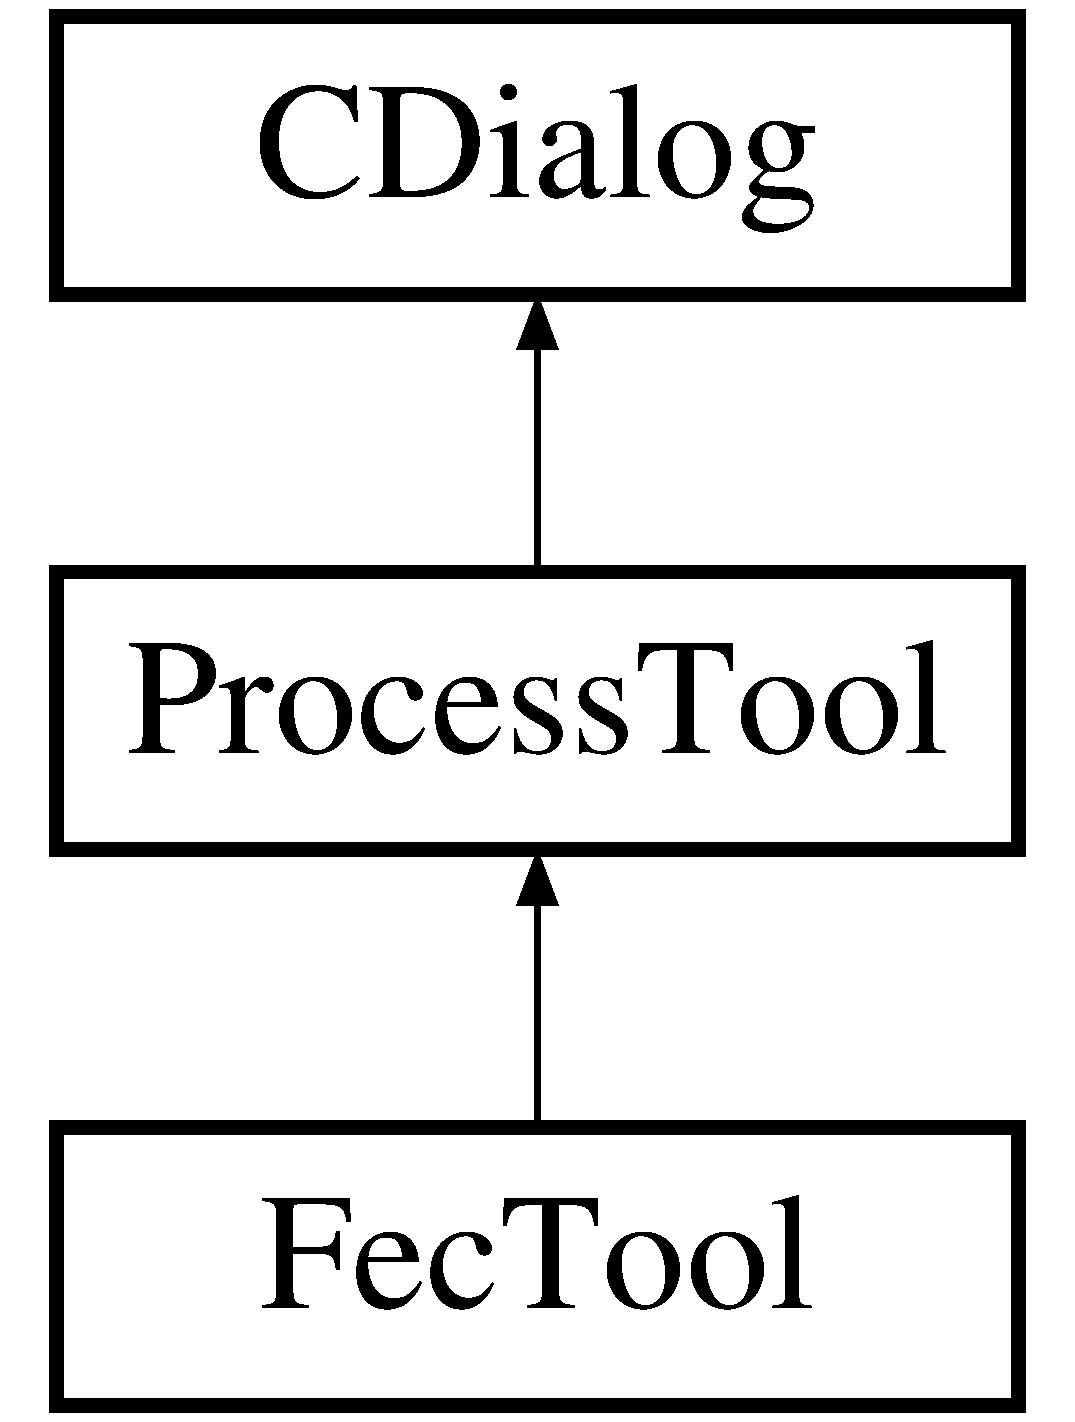
\includegraphics[height=3.000000cm]{class_fec_tool}
\end{center}
\end{figure}
\subsection*{Public Types}
\begin{DoxyCompactItemize}
\item 
\mbox{\Hypertarget{class_fec_tool_ac41f0ce67dfecf0eb6c067e60f9e7e42}\label{class_fec_tool_ac41f0ce67dfecf0eb6c067e60f9e7e42}} 
enum \{ {\bfseries I\+DD} = I\+D\+D\+\_\+\+F\+EC
 \}
\end{DoxyCompactItemize}
\subsection*{Public Member Functions}
\begin{DoxyCompactItemize}
\item 
\mbox{\Hypertarget{class_fec_tool_ad2b7046951f2aa7494e9b1a3f22bed02}\label{class_fec_tool_ad2b7046951f2aa7494e9b1a3f22bed02}} 
{\bfseries Fec\+Tool} (C\+Wnd $\ast$p\+Parent=N\+U\+LL)
\item 
virtual void \mbox{\hyperlink{class_fec_tool_acd6cd4230cb79fe0cb1053c588f91806}{Set\+Param}} (\mbox{\hyperlink{class_process_wrap}{Process\+Wrap}} $\ast$p\+Param)
\item 
virtual \mbox{\hyperlink{class_process_wrap}{Process\+Wrap}} $\ast$ \mbox{\hyperlink{class_fec_tool_acccda5a312354ec0dcd215de8ed7ac03}{Get\+Param}} ()
\item 
virtual void \mbox{\hyperlink{class_fec_tool_ac99805fa120b8bb7a21fc08382a875c1}{Set\+Img\+File}} (Img\+File $\ast$p\+Image)
\item 
\mbox{\Hypertarget{class_fec_tool_a7a6d4107c9007878d2df2fb7da24942d}\label{class_fec_tool_a7a6d4107c9007878d2df2fb7da24942d}} 
afx\+\_\+msg void {\bfseries On\+Deltapos\+Center\+X\+Spin} (N\+M\+H\+DR $\ast$p\+N\+M\+H\+DR, L\+R\+E\+S\+U\+LT $\ast$p\+Result)
\item 
\mbox{\Hypertarget{class_fec_tool_ac4a93c620e0c86c63f13c0ae8213d367}\label{class_fec_tool_ac4a93c620e0c86c63f13c0ae8213d367}} 
afx\+\_\+msg void {\bfseries On\+Deltapos\+Center\+Y\+Spin} (N\+M\+H\+DR $\ast$p\+N\+M\+H\+DR, L\+R\+E\+S\+U\+LT $\ast$p\+Result)
\item 
\mbox{\Hypertarget{class_fec_tool_adddbc3e62af06a502e71823b7e2d04ef}\label{class_fec_tool_adddbc3e62af06a502e71823b7e2d04ef}} 
afx\+\_\+msg void {\bfseries On\+Deltapos\+Radius\+X\+Spin} (N\+M\+H\+DR $\ast$p\+N\+M\+H\+DR, L\+R\+E\+S\+U\+LT $\ast$p\+Result)
\item 
\mbox{\Hypertarget{class_fec_tool_acfe7023da87b248e66ba244817c7ff4f}\label{class_fec_tool_acfe7023da87b248e66ba244817c7ff4f}} 
afx\+\_\+msg void {\bfseries On\+Deltapos\+Radius\+Y\+Spin} (N\+M\+H\+DR $\ast$p\+N\+M\+H\+DR, L\+R\+E\+S\+U\+LT $\ast$p\+Result)
\item 
\mbox{\Hypertarget{class_fec_tool_a8f3294300b4ee2cbe52cac21b0d4dc43}\label{class_fec_tool_a8f3294300b4ee2cbe52cac21b0d4dc43}} 
afx\+\_\+msg void {\bfseries On\+Deltapos\+Curve\+H\+Spin} (N\+M\+H\+DR $\ast$p\+N\+M\+H\+DR, L\+R\+E\+S\+U\+LT $\ast$p\+Result)
\item 
\mbox{\Hypertarget{class_fec_tool_a2a65a052c43c27968a6ef6eb93d7095d}\label{class_fec_tool_a2a65a052c43c27968a6ef6eb93d7095d}} 
afx\+\_\+msg void {\bfseries On\+Deltapos\+Curve\+V\+Spin} (N\+M\+H\+DR $\ast$p\+N\+M\+H\+DR, L\+R\+E\+S\+U\+LT $\ast$p\+Result)
\item 
\mbox{\Hypertarget{class_fec_tool_af2aa98a5d986106082994ffe5dfa8219}\label{class_fec_tool_af2aa98a5d986106082994ffe5dfa8219}} 
afx\+\_\+msg void {\bfseries On\+Deltapos\+Fov\+H\+Spin} (N\+M\+H\+DR $\ast$p\+N\+M\+H\+DR, L\+R\+E\+S\+U\+LT $\ast$p\+Result)
\item 
\mbox{\Hypertarget{class_fec_tool_a27a6d44bc322df9abfa6a4dab93e796f}\label{class_fec_tool_a27a6d44bc322df9abfa6a4dab93e796f}} 
afx\+\_\+msg void {\bfseries On\+Deltapos\+Fov\+V\+Spin} (N\+M\+H\+DR $\ast$p\+N\+M\+H\+DR, L\+R\+E\+S\+U\+LT $\ast$p\+Result)
\item 
\mbox{\Hypertarget{class_fec_tool_a7cfdea1e3f18cc09d96c8f70856fefa6}\label{class_fec_tool_a7cfdea1e3f18cc09d96c8f70856fefa6}} 
afx\+\_\+msg void {\bfseries On\+Deltapos\+Pitch\+Spin} (N\+M\+H\+DR $\ast$p\+N\+M\+H\+DR, L\+R\+E\+S\+U\+LT $\ast$p\+Result)
\item 
\mbox{\Hypertarget{class_fec_tool_a32e53997d8fa0670b379e56fd3f5d869}\label{class_fec_tool_a32e53997d8fa0670b379e56fd3f5d869}} 
afx\+\_\+msg void {\bfseries On\+Deltapos\+Yaw\+Spin} (N\+M\+H\+DR $\ast$p\+N\+M\+H\+DR, L\+R\+E\+S\+U\+LT $\ast$p\+Result)
\item 
\mbox{\Hypertarget{class_fec_tool_af6793729b332372e36e7cfc3f0ccbedf}\label{class_fec_tool_af6793729b332372e36e7cfc3f0ccbedf}} 
afx\+\_\+msg void {\bfseries On\+Deltapos\+Roll\+Spin} (N\+M\+H\+DR $\ast$p\+N\+M\+H\+DR, L\+R\+E\+S\+U\+LT $\ast$p\+Result)
\item 
\mbox{\Hypertarget{class_fec_tool_ac257463f34fc4bc4bf2a49c9c5ad3253}\label{class_fec_tool_ac257463f34fc4bc4bf2a49c9c5ad3253}} 
afx\+\_\+msg void {\bfseries On\+Bn\+Clicked\+Ok} ()
\end{DoxyCompactItemize}
\subsection*{Protected Member Functions}
\begin{DoxyCompactItemize}
\item 
\mbox{\Hypertarget{class_fec_tool_a206c20426c1448c7fa2a1cb9081dbb93}\label{class_fec_tool_a206c20426c1448c7fa2a1cb9081dbb93}} 
void {\bfseries Update\+Data} (B\+O\+OL b\+Save\+And\+Validate=T\+R\+UE)
\end{DoxyCompactItemize}
\subsection*{Additional Inherited Members}


\subsection{Detailed Description}
\mbox{\hyperlink{class_fec_tool}{Fec\+Tool}} is used to control the settings of F\+EC process with UI in a dialog box. This class sends the parameters to a \mbox{\hyperlink{class_fec_view}{Fec\+View}} to display the resulted image. It also connects to a \mbox{\hyperlink{class_fec_wrap}{Fec\+Wrap}} class to maintain the F\+EC process related parameters and L\+UT data. 

\subsection{Member Function Documentation}
\mbox{\Hypertarget{class_fec_tool_acccda5a312354ec0dcd215de8ed7ac03}\label{class_fec_tool_acccda5a312354ec0dcd215de8ed7ac03}} 
\index{Fec\+Tool@{Fec\+Tool}!Get\+Param@{Get\+Param}}
\index{Get\+Param@{Get\+Param}!Fec\+Tool@{Fec\+Tool}}
\subsubsection{\texorpdfstring{Get\+Param()}{GetParam()}}
{\footnotesize\ttfamily \mbox{\hyperlink{class_process_wrap}{Process\+Wrap}} $\ast$ Fec\+Tool\+::\+Get\+Param (\begin{DoxyParamCaption}{ }\end{DoxyParamCaption})\hspace{0.3cm}{\ttfamily [virtual]}}

Gets the \mbox{\hyperlink{class_process_wrap}{Process\+Wrap}} class pointer of the process tool. 

Reimplemented from \mbox{\hyperlink{class_process_tool_a355ebcf991f86f59f4241ea4345547fc}{Process\+Tool}}.

\mbox{\Hypertarget{class_fec_tool_ac99805fa120b8bb7a21fc08382a875c1}\label{class_fec_tool_ac99805fa120b8bb7a21fc08382a875c1}} 
\index{Fec\+Tool@{Fec\+Tool}!Set\+Img\+File@{Set\+Img\+File}}
\index{Set\+Img\+File@{Set\+Img\+File}!Fec\+Tool@{Fec\+Tool}}
\subsubsection{\texorpdfstring{Set\+Img\+File()}{SetImgFile()}}
{\footnotesize\ttfamily void Fec\+Tool\+::\+Set\+Img\+File (\begin{DoxyParamCaption}\item[{Img\+File $\ast$}]{p\+Image }\end{DoxyParamCaption})\hspace{0.3cm}{\ttfamily [virtual]}}

Sets the image to be processed from. The processed imaged won\textquotesingle{}t replace this original image. 

Reimplemented from \mbox{\hyperlink{class_process_tool_a178bc06abf5a20220bd2306a14708a93}{Process\+Tool}}.

\mbox{\Hypertarget{class_fec_tool_acd6cd4230cb79fe0cb1053c588f91806}\label{class_fec_tool_acd6cd4230cb79fe0cb1053c588f91806}} 
\index{Fec\+Tool@{Fec\+Tool}!Set\+Param@{Set\+Param}}
\index{Set\+Param@{Set\+Param}!Fec\+Tool@{Fec\+Tool}}
\subsubsection{\texorpdfstring{Set\+Param()}{SetParam()}}
{\footnotesize\ttfamily void Fec\+Tool\+::\+Set\+Param (\begin{DoxyParamCaption}\item[{\mbox{\hyperlink{class_process_wrap}{Process\+Wrap}} $\ast$}]{p\+Param }\end{DoxyParamCaption})\hspace{0.3cm}{\ttfamily [virtual]}}

Copys contents of process parameters into related \mbox{\hyperlink{class_process_wrap}{Process\+Wrap}}. 

Reimplemented from \mbox{\hyperlink{class_process_tool_a50caa175198cece00b39a146715bf3eb}{Process\+Tool}}.



The documentation for this class was generated from the following files\+:\begin{DoxyCompactItemize}
\item 
i\+Optics/\mbox{\hyperlink{_fec_tool_8h}{Fec\+Tool.\+h}}\item 
i\+Optics/Fec\+Tool.\+cpp\end{DoxyCompactItemize}

\hypertarget{class_fec_view}{}\section{Fec\+View Class Reference}
\label{class_fec_view}\index{Fec\+View@{Fec\+View}}


\mbox{\hyperlink{class_fec_view}{Fec\+View}} is the image viewer for F\+EC processing image. It handles the video rendering process by the specified process. It is controlled by its process correspondent \mbox{\hyperlink{class_fec_tool}{Fec\+Tool}}. It also can display gride lines on the image window.  




{\ttfamily \#include $<$Fec\+View.\+h$>$}

Inheritance diagram for Fec\+View\+:\begin{figure}[H]
\begin{center}
\leavevmode
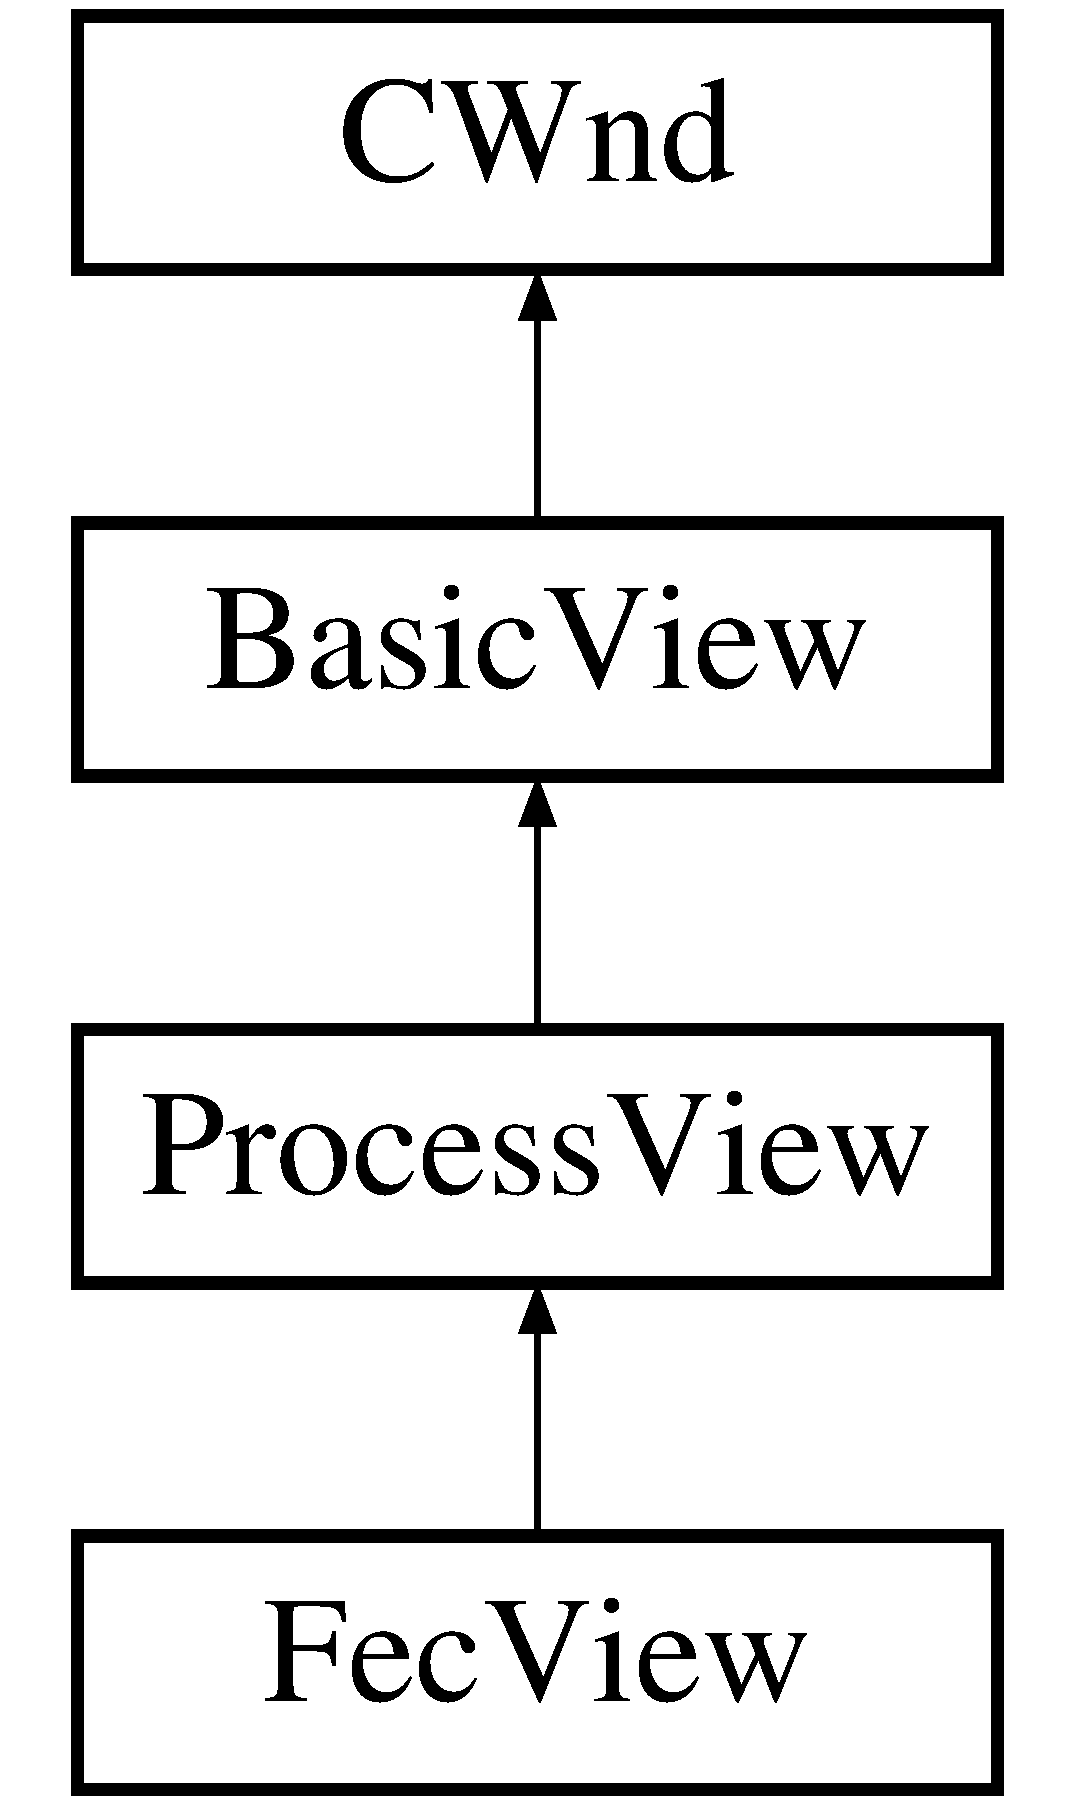
\includegraphics[height=4.000000cm]{class_fec_view}
\end{center}
\end{figure}
\subsection*{Public Member Functions}
\begin{DoxyCompactItemize}
\item 
\mbox{\Hypertarget{class_fec_view_a8d9efd2c95cbd8807518735d46ae4eee}\label{class_fec_view_a8d9efd2c95cbd8807518735d46ae4eee}} 
virtual void {\bfseries Set\+Param} (\mbox{\hyperlink{class_process_wrap}{Process\+Wrap}} $\ast$p\+Wrapper)
\item 
\mbox{\Hypertarget{class_fec_view_a83ed54e633d3b45d4134dcf0d8f8941e}\label{class_fec_view_a83ed54e633d3b45d4134dcf0d8f8941e}} 
afx\+\_\+msg void {\bfseries On\+Preview} ()
\end{DoxyCompactItemize}
\subsection*{Public Attributes}
\begin{DoxyCompactItemize}
\item 
\mbox{\Hypertarget{class_fec_view_afafd7be607439614e4627e085e203f04}\label{class_fec_view_afafd7be607439614e4627e085e203f04}} 
\mbox{\hyperlink{class_fec_wrap}{Fec\+Wrap}} $\ast$ {\bfseries m\+\_\+p\+Param\+Ref}
\end{DoxyCompactItemize}
\subsection*{Protected Member Functions}
\begin{DoxyCompactItemize}
\item 
\mbox{\Hypertarget{class_fec_view_a10a85bda7c6440797e16ecf9aba87233}\label{class_fec_view_a10a85bda7c6440797e16ecf9aba87233}} 
virtual B\+O\+OL {\bfseries Pos\+Map} (int u, int v, float \&x, float \&y)
\item 
\mbox{\Hypertarget{class_fec_view_a15de2adcdfb141d22ff96cb6d5fdb607}\label{class_fec_view_a15de2adcdfb141d22ff96cb6d5fdb607}} 
virtual C\+O\+L\+O\+R\+R\+EF {\bfseries Get\+Color} (B\+Y\+TE $\ast$p\+Src, int stride, float x, float y)
\end{DoxyCompactItemize}
\subsection*{Additional Inherited Members}


\subsection{Detailed Description}
\mbox{\hyperlink{class_fec_view}{Fec\+View}} is the image viewer for F\+EC processing image. It handles the video rendering process by the specified process. It is controlled by its process correspondent \mbox{\hyperlink{class_fec_tool}{Fec\+Tool}}. It also can display gride lines on the image window. 

\begin{DoxySeeAlso}{See also}
\mbox{\hyperlink{class_fec_tool}{Fec\+Tool}}. 
\end{DoxySeeAlso}


The documentation for this class was generated from the following files\+:\begin{DoxyCompactItemize}
\item 
i\+Optics/\mbox{\hyperlink{_fec_view_8h}{Fec\+View.\+h}}\item 
i\+Optics/Fec\+View.\+cpp\end{DoxyCompactItemize}

\hypertarget{class_fec_wrap}{}\section{Fec\+Wrap Class Reference}
\label{class_fec_wrap}\index{Fec\+Wrap@{Fec\+Wrap}}


F\+EC process parameters wrapper This class wrap F\+EC parameters and L\+UT table, as well as L\+UT generating function.  




{\ttfamily \#include $<$Fec\+Tool.\+h$>$}

Inheritance diagram for Fec\+Wrap\+:\begin{figure}[H]
\begin{center}
\leavevmode
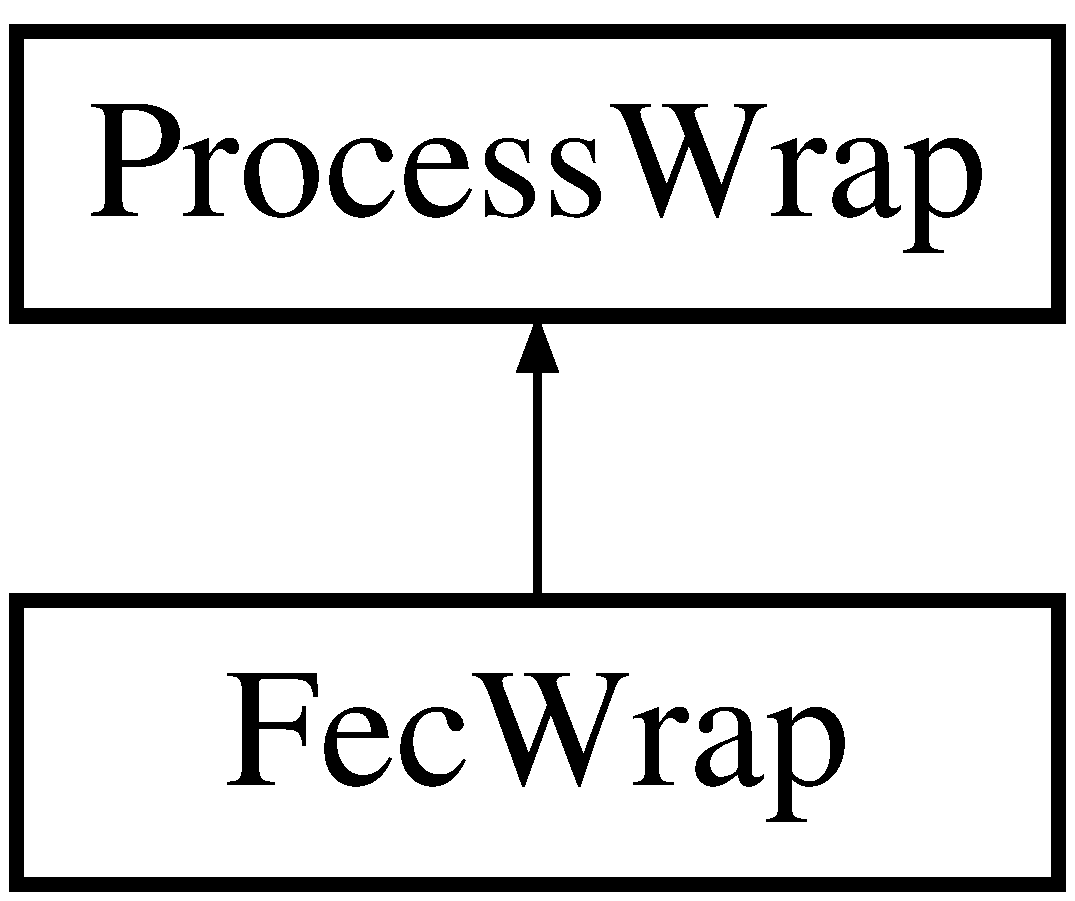
\includegraphics[height=2.000000cm]{class_fec_wrap}
\end{center}
\end{figure}
\subsection*{Public Member Functions}
\begin{DoxyCompactItemize}
\item 
virtual void \mbox{\hyperlink{class_fec_wrap_a989dbae7d3f292f4e686eee8f19a1ad7}{Set\+Param}} (void $\ast$p\+Param)
\item 
virtual void \mbox{\hyperlink{class_fec_wrap_ac1c213fd03716ce0bb6430e2d2bf7962}{Make\+Map\+Table}} ()
\item 
virtual B\+O\+OL \mbox{\hyperlink{class_fec_wrap_a50575c4f361b71e6de2e8c1073b4a26a}{Pos\+Map}} (int u, int v, float \&x, float \&y)
\item 
virtual B\+O\+OL \mbox{\hyperlink{class_fec_wrap_abd377e205b42ec6725293c3c9ff76a34}{Save\+Parameter}} (L\+P\+C\+T\+S\+TR filename)
\item 
virtual B\+O\+OL \mbox{\hyperlink{class_fec_wrap_a3f55d86b6b99108b360b66d1d180a66c}{Load\+Parameter}} (L\+P\+C\+T\+S\+TR filename)
\end{DoxyCompactItemize}
\subsection*{Friends}
\begin{DoxyCompactItemize}
\item 
\mbox{\Hypertarget{class_fec_wrap_aee89ac5ae8a164efc12e3ffdba0f5cc6}\label{class_fec_wrap_aee89ac5ae8a164efc12e3ffdba0f5cc6}} 
class {\bfseries Fec\+Tool}
\item 
\mbox{\Hypertarget{class_fec_wrap_a6bf8ef1e5b278887294b17a7aa714e7b}\label{class_fec_wrap_a6bf8ef1e5b278887294b17a7aa714e7b}} 
class {\bfseries Fec\+View}
\item 
\mbox{\Hypertarget{class_fec_wrap_a8dfb14a6a11e1fad081be201e28a0f37}\label{class_fec_wrap_a8dfb14a6a11e1fad081be201e28a0f37}} 
class {\bfseries Fec\+Gride}
\end{DoxyCompactItemize}
\subsection*{Additional Inherited Members}


\subsection{Detailed Description}
F\+EC process parameters wrapper This class wrap F\+EC parameters and L\+UT table, as well as L\+UT generating function. 

\begin{DoxySeeAlso}{See also}
\mbox{\hyperlink{class_fec_view}{Fec\+View}} \mbox{\hyperlink{class_process_wrap}{Process\+Wrap}} 
\end{DoxySeeAlso}


\subsection{Member Function Documentation}
\mbox{\Hypertarget{class_fec_wrap_a3f55d86b6b99108b360b66d1d180a66c}\label{class_fec_wrap_a3f55d86b6b99108b360b66d1d180a66c}} 
\index{Fec\+Wrap@{Fec\+Wrap}!Load\+Parameter@{Load\+Parameter}}
\index{Load\+Parameter@{Load\+Parameter}!Fec\+Wrap@{Fec\+Wrap}}
\subsubsection{\texorpdfstring{Load\+Parameter()}{LoadParameter()}}
{\footnotesize\ttfamily B\+O\+OL Fec\+Wrap\+::\+Load\+Parameter (\begin{DoxyParamCaption}\item[{L\+P\+C\+T\+S\+TR}]{filename }\end{DoxyParamCaption})\hspace{0.3cm}{\ttfamily [virtual]}}

Read process specified parameters from a file. The format of data can be defined dependently by the correspondent \mbox{\hyperlink{class_process_wrap}{Process\+Wrap}} class. 

Implements \mbox{\hyperlink{class_process_wrap_a1cb75a423ff8f5ef736fc00a34792493}{Process\+Wrap}}.

\mbox{\Hypertarget{class_fec_wrap_ac1c213fd03716ce0bb6430e2d2bf7962}\label{class_fec_wrap_ac1c213fd03716ce0bb6430e2d2bf7962}} 
\index{Fec\+Wrap@{Fec\+Wrap}!Make\+Map\+Table@{Make\+Map\+Table}}
\index{Make\+Map\+Table@{Make\+Map\+Table}!Fec\+Wrap@{Fec\+Wrap}}
\subsubsection{\texorpdfstring{Make\+Map\+Table()}{MakeMapTable()}}
{\footnotesize\ttfamily void Fec\+Wrap\+::\+Make\+Map\+Table (\begin{DoxyParamCaption}{ }\end{DoxyParamCaption})\hspace{0.3cm}{\ttfamily [virtual]}}

Create the L\+UT data according the internal Fec\+Param 

Implements \mbox{\hyperlink{class_process_wrap_a22910a91f52147b8631b7e880509996e}{Process\+Wrap}}.

\mbox{\Hypertarget{class_fec_wrap_a50575c4f361b71e6de2e8c1073b4a26a}\label{class_fec_wrap_a50575c4f361b71e6de2e8c1073b4a26a}} 
\index{Fec\+Wrap@{Fec\+Wrap}!Pos\+Map@{Pos\+Map}}
\index{Pos\+Map@{Pos\+Map}!Fec\+Wrap@{Fec\+Wrap}}
\subsubsection{\texorpdfstring{Pos\+Map()}{PosMap()}}
{\footnotesize\ttfamily B\+O\+OL Fec\+Wrap\+::\+Pos\+Map (\begin{DoxyParamCaption}\item[{int}]{u,  }\item[{int}]{v,  }\item[{float \&}]{x,  }\item[{float \&}]{y }\end{DoxyParamCaption})\hspace{0.3cm}{\ttfamily [virtual]}}

Position mapping from processed image to original image 
\begin{DoxyParams}[1]{Parameters}
\mbox{\tt in}  & {\em u} & \mbox{[}0$\sim$sz\+Output.cx) in rocessed image \\
\hline
\mbox{\tt in}  & {\em v} & \mbox{[}0$\sim$sz\+Output.cy) in rocessed image \\
\hline
\mbox{\tt out}  & {\em x} & \mbox{[}0$\sim$sz\+Input.cx) in rocessed image \\
\hline
\mbox{\tt out}  & {\em y} & \mbox{[}0$\sim$sz\+Input.cy) in rocessed image \\
\hline
\end{DoxyParams}


Implements \mbox{\hyperlink{class_process_wrap_a536c940a16b6331109aa5d30763974fe}{Process\+Wrap}}.

\mbox{\Hypertarget{class_fec_wrap_abd377e205b42ec6725293c3c9ff76a34}\label{class_fec_wrap_abd377e205b42ec6725293c3c9ff76a34}} 
\index{Fec\+Wrap@{Fec\+Wrap}!Save\+Parameter@{Save\+Parameter}}
\index{Save\+Parameter@{Save\+Parameter}!Fec\+Wrap@{Fec\+Wrap}}
\subsubsection{\texorpdfstring{Save\+Parameter()}{SaveParameter()}}
{\footnotesize\ttfamily B\+O\+OL Fec\+Wrap\+::\+Save\+Parameter (\begin{DoxyParamCaption}\item[{L\+P\+C\+T\+S\+TR}]{filename }\end{DoxyParamCaption})\hspace{0.3cm}{\ttfamily [virtual]}}

Save process specified parameters in a file. The format of data can be defined dependently in this function. 

Implements \mbox{\hyperlink{class_process_wrap_aa5d4361a42a7a65cac877beb6d4ffa97}{Process\+Wrap}}.

\mbox{\Hypertarget{class_fec_wrap_a989dbae7d3f292f4e686eee8f19a1ad7}\label{class_fec_wrap_a989dbae7d3f292f4e686eee8f19a1ad7}} 
\index{Fec\+Wrap@{Fec\+Wrap}!Set\+Param@{Set\+Param}}
\index{Set\+Param@{Set\+Param}!Fec\+Wrap@{Fec\+Wrap}}
\subsubsection{\texorpdfstring{Set\+Param()}{SetParam()}}
{\footnotesize\ttfamily void Fec\+Wrap\+::\+Set\+Param (\begin{DoxyParamCaption}\item[{void $\ast$}]{p\+Param }\end{DoxyParamCaption})\hspace{0.3cm}{\ttfamily [virtual]}}

Sets F\+EC processing prameters, which is copied to class members and generate the L\+UT data. 
\begin{DoxyParams}{Parameters}
{\em p\+Param} & pointer to Fec\+Param. \\
\hline
\end{DoxyParams}


Reimplemented from \mbox{\hyperlink{class_process_wrap_a6c7130837d4713b0462f42cfc25aca98}{Process\+Wrap}}.



The documentation for this class was generated from the following files\+:\begin{DoxyCompactItemize}
\item 
i\+Optics/\mbox{\hyperlink{_fec_tool_8h}{Fec\+Tool.\+h}}\item 
i\+Optics/Fec\+Tool.\+cpp\end{DoxyCompactItemize}

\hypertarget{class_gride}{}\section{Gride Class Reference}
\label{class_gride}\index{Gride@{Gride}}
Inheritance diagram for Gride\+:\begin{figure}[H]
\begin{center}
\leavevmode
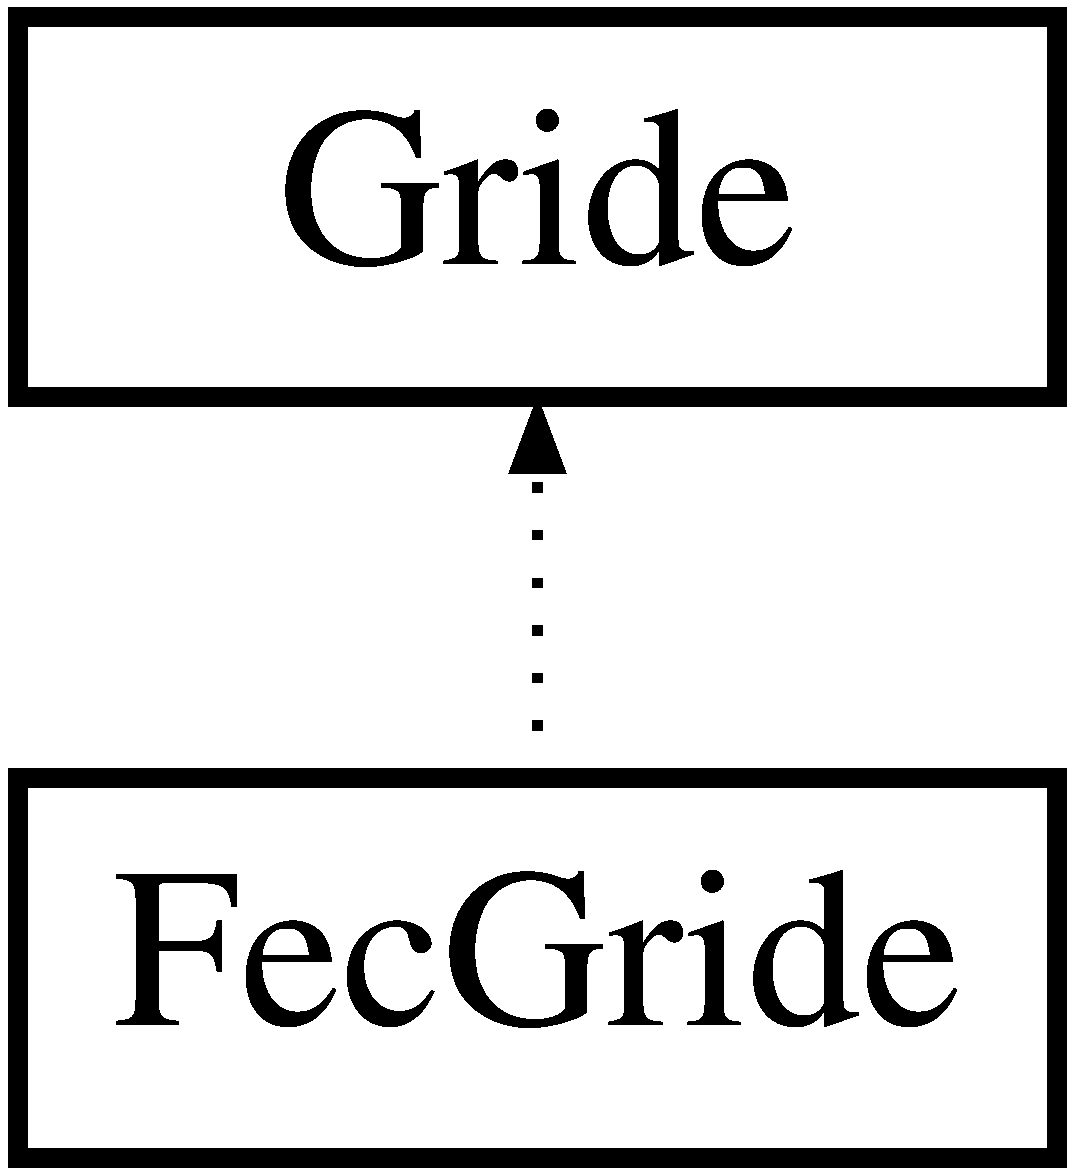
\includegraphics[height=2.000000cm]{class_gride}
\end{center}
\end{figure}
\subsection*{Public Member Functions}
\begin{DoxyCompactItemize}
\item 
\mbox{\Hypertarget{class_gride_a5191e375eefed134243a36b19cc29e4b}\label{class_gride_a5191e375eefed134243a36b19cc29e4b}} 
{\bfseries Gride} (C\+O\+L\+O\+R\+R\+EF color)
\item 
\mbox{\Hypertarget{class_gride_a437b35e279bbe1639c8375e9cf8f5e83}\label{class_gride_a437b35e279bbe1639c8375e9cf8f5e83}} 
virtual void {\bfseries Draw} (C\+DC $\ast$p\+DC)
\item 
\mbox{\Hypertarget{class_gride_af033f138fd823c16846699d4722e0d86}\label{class_gride_af033f138fd823c16846699d4722e0d86}} 
virtual void {\bfseries Set\+Param} (void $\ast$p\+Param)
\item 
\mbox{\Hypertarget{class_gride_a8bf37bf5afa6de5bc022ed049fec6eab}\label{class_gride_a8bf37bf5afa6de5bc022ed049fec6eab}} 
void {\bfseries Set\+Image\+Area} (R\+E\+CT \&rc\+Range)
\item 
\mbox{\Hypertarget{class_gride_a06e001fe22bd5702315fc1d710dc5f16}\label{class_gride_a06e001fe22bd5702315fc1d710dc5f16}} 
void {\bfseries Set\+View\+Port} (R\+E\+CT \&rc\+View\+Port)
\end{DoxyCompactItemize}
\subsection*{Protected Attributes}
\begin{DoxyCompactItemize}
\item 
\mbox{\Hypertarget{class_gride_a7ea4a4f620430655d7a2580d17ab5018}\label{class_gride_a7ea4a4f620430655d7a2580d17ab5018}} 
R\+E\+CT {\bfseries m\+\_\+rc\+View\+Port}
\item 
\mbox{\Hypertarget{class_gride_a6c665805c7bccae37782bc91ccabf03e}\label{class_gride_a6c665805c7bccae37782bc91ccabf03e}} 
R\+E\+CT {\bfseries m\+\_\+rc\+Range}
\item 
\mbox{\Hypertarget{class_gride_a0ab3e516224b88c29fe59883ed8ba132}\label{class_gride_a0ab3e516224b88c29fe59883ed8ba132}} 
C\+O\+L\+O\+R\+R\+EF {\bfseries m\+\_\+color}
\item 
\mbox{\Hypertarget{class_gride_afc79ddb62399c63257357a2f380d7509}\label{class_gride_afc79ddb62399c63257357a2f380d7509}} 
int {\bfseries m\+\_\+n\+Interval}
\item 
\mbox{\Hypertarget{class_gride_a0d95020c7d18231961a105f97e124953}\label{class_gride_a0d95020c7d18231961a105f97e124953}} 
int {\bfseries m\+\_\+n\+Divider}
\end{DoxyCompactItemize}


The documentation for this class was generated from the following files\+:\begin{DoxyCompactItemize}
\item 
i\+Optics/Gride.\+h\item 
i\+Optics/Gride.\+cpp\end{DoxyCompactItemize}

\hypertarget{class_homo_tool}{}\section{Homo\+Tool Class Reference}
\label{class_homo_tool}\index{Homo\+Tool@{Homo\+Tool}}
Inheritance diagram for Homo\+Tool\+:\begin{figure}[H]
\begin{center}
\leavevmode
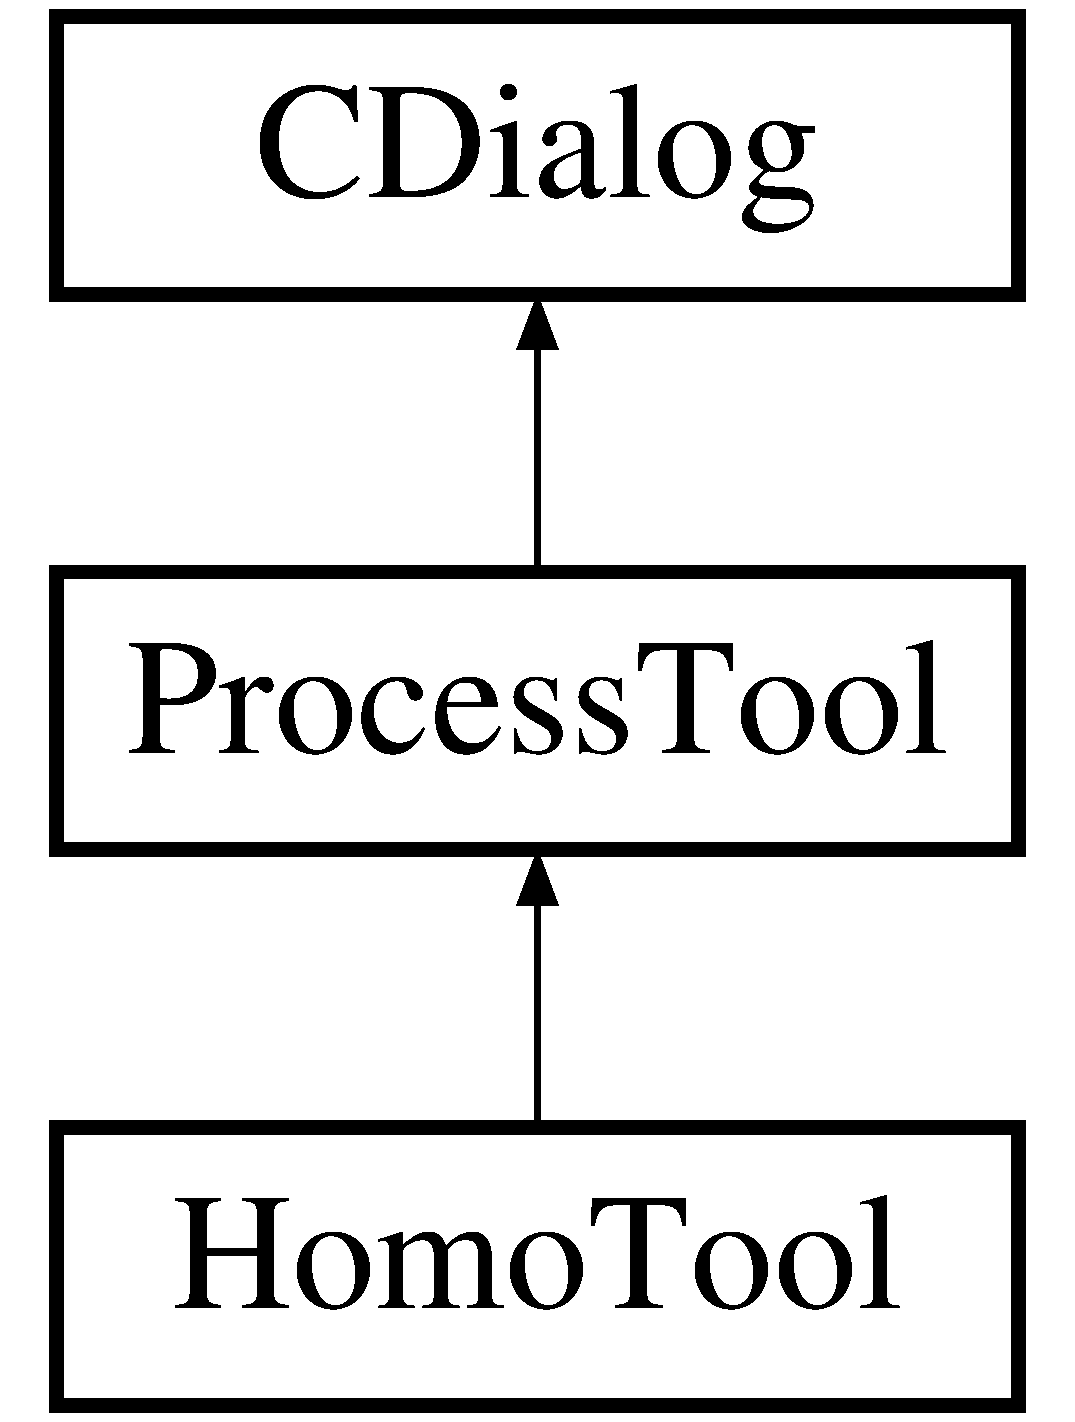
\includegraphics[height=3.000000cm]{class_homo_tool}
\end{center}
\end{figure}
\subsection*{Public Types}
\begin{DoxyCompactItemize}
\item 
\mbox{\Hypertarget{class_homo_tool_a14de69e679bae0adc7a2ebfabd62c878}\label{class_homo_tool_a14de69e679bae0adc7a2ebfabd62c878}} 
enum \{ {\bfseries I\+DD} = I\+D\+D\+\_\+\+H\+O\+MO
 \}
\end{DoxyCompactItemize}
\subsection*{Public Member Functions}
\begin{DoxyCompactItemize}
\item 
\mbox{\Hypertarget{class_homo_tool_a9d149e537ecd9d22a6dea13a2ebfdfd3}\label{class_homo_tool_a9d149e537ecd9d22a6dea13a2ebfdfd3}} 
{\bfseries Homo\+Tool} (C\+Wnd $\ast$p\+Parent=N\+U\+LL)
\item 
virtual void \mbox{\hyperlink{class_homo_tool_a69965855ba23da88abe7903ad58c20c6}{Set\+Param}} (\mbox{\hyperlink{class_process_wrap}{Process\+Wrap}} $\ast$p\+Param)
\item 
virtual \mbox{\hyperlink{class_process_wrap}{Process\+Wrap}} $\ast$ \mbox{\hyperlink{class_homo_tool_a497eb4f1812d3f38ea6657c35d64bf31}{Get\+Param}} ()
\item 
virtual void \mbox{\hyperlink{class_homo_tool_af43fe8ae0732dffbeb35b59058509af2}{Set\+Img\+File}} (Img\+File $\ast$p\+Image)
\end{DoxyCompactItemize}
\subsection*{Protected Member Functions}
\begin{DoxyCompactItemize}
\item 
\mbox{\Hypertarget{class_homo_tool_a023cbc511c52831d2b7144695821f439}\label{class_homo_tool_a023cbc511c52831d2b7144695821f439}} 
virtual void {\bfseries Do\+Data\+Exchange} (C\+Data\+Exchange $\ast$p\+DX)
\end{DoxyCompactItemize}
\subsection*{Additional Inherited Members}


\subsection{Member Function Documentation}
\mbox{\Hypertarget{class_homo_tool_a497eb4f1812d3f38ea6657c35d64bf31}\label{class_homo_tool_a497eb4f1812d3f38ea6657c35d64bf31}} 
\index{Homo\+Tool@{Homo\+Tool}!Get\+Param@{Get\+Param}}
\index{Get\+Param@{Get\+Param}!Homo\+Tool@{Homo\+Tool}}
\subsubsection{\texorpdfstring{Get\+Param()}{GetParam()}}
{\footnotesize\ttfamily virtual \mbox{\hyperlink{class_process_wrap}{Process\+Wrap}}$\ast$ Homo\+Tool\+::\+Get\+Param (\begin{DoxyParamCaption}{ }\end{DoxyParamCaption})\hspace{0.3cm}{\ttfamily [inline]}, {\ttfamily [virtual]}}

Gets the \mbox{\hyperlink{class_process_wrap}{Process\+Wrap}} class pointer of the process tool. 

Reimplemented from \mbox{\hyperlink{class_process_tool_a355ebcf991f86f59f4241ea4345547fc}{Process\+Tool}}.

\mbox{\Hypertarget{class_homo_tool_af43fe8ae0732dffbeb35b59058509af2}\label{class_homo_tool_af43fe8ae0732dffbeb35b59058509af2}} 
\index{Homo\+Tool@{Homo\+Tool}!Set\+Img\+File@{Set\+Img\+File}}
\index{Set\+Img\+File@{Set\+Img\+File}!Homo\+Tool@{Homo\+Tool}}
\subsubsection{\texorpdfstring{Set\+Img\+File()}{SetImgFile()}}
{\footnotesize\ttfamily void Homo\+Tool\+::\+Set\+Img\+File (\begin{DoxyParamCaption}\item[{Img\+File $\ast$}]{p\+Image }\end{DoxyParamCaption})\hspace{0.3cm}{\ttfamily [virtual]}}

Sets the image to be processed from. The processed imaged won\textquotesingle{}t replace this original image. 

Reimplemented from \mbox{\hyperlink{class_process_tool_a178bc06abf5a20220bd2306a14708a93}{Process\+Tool}}.

\mbox{\Hypertarget{class_homo_tool_a69965855ba23da88abe7903ad58c20c6}\label{class_homo_tool_a69965855ba23da88abe7903ad58c20c6}} 
\index{Homo\+Tool@{Homo\+Tool}!Set\+Param@{Set\+Param}}
\index{Set\+Param@{Set\+Param}!Homo\+Tool@{Homo\+Tool}}
\subsubsection{\texorpdfstring{Set\+Param()}{SetParam()}}
{\footnotesize\ttfamily virtual void Homo\+Tool\+::\+Set\+Param (\begin{DoxyParamCaption}\item[{\mbox{\hyperlink{class_process_wrap}{Process\+Wrap}} $\ast$}]{p\+Param }\end{DoxyParamCaption})\hspace{0.3cm}{\ttfamily [inline]}, {\ttfamily [virtual]}}

Copys contents of process parameters into related \mbox{\hyperlink{class_process_wrap}{Process\+Wrap}}. 

Reimplemented from \mbox{\hyperlink{class_process_tool_a50caa175198cece00b39a146715bf3eb}{Process\+Tool}}.



The documentation for this class was generated from the following files\+:\begin{DoxyCompactItemize}
\item 
i\+Optics/Homo\+Tool.\+h\item 
i\+Optics/Homo\+Tool.\+cpp\end{DoxyCompactItemize}

\hypertarget{class_homo_view}{}\section{Homo\+View Class Reference}
\label{class_homo_view}\index{Homo\+View@{Homo\+View}}


\mbox{\hyperlink{class_homo_view}{Homo\+View}} is the image viewer for Homography matrix processing image. It handles the video rendering process by the specified process. It is controlled by its process correspondent \mbox{\hyperlink{class_homo_tool}{Homo\+Tool}}. It also can display gride lines on the image window.  




{\ttfamily \#include $<$Homo\+View.\+h$>$}

Inheritance diagram for Homo\+View\+:\begin{figure}[H]
\begin{center}
\leavevmode
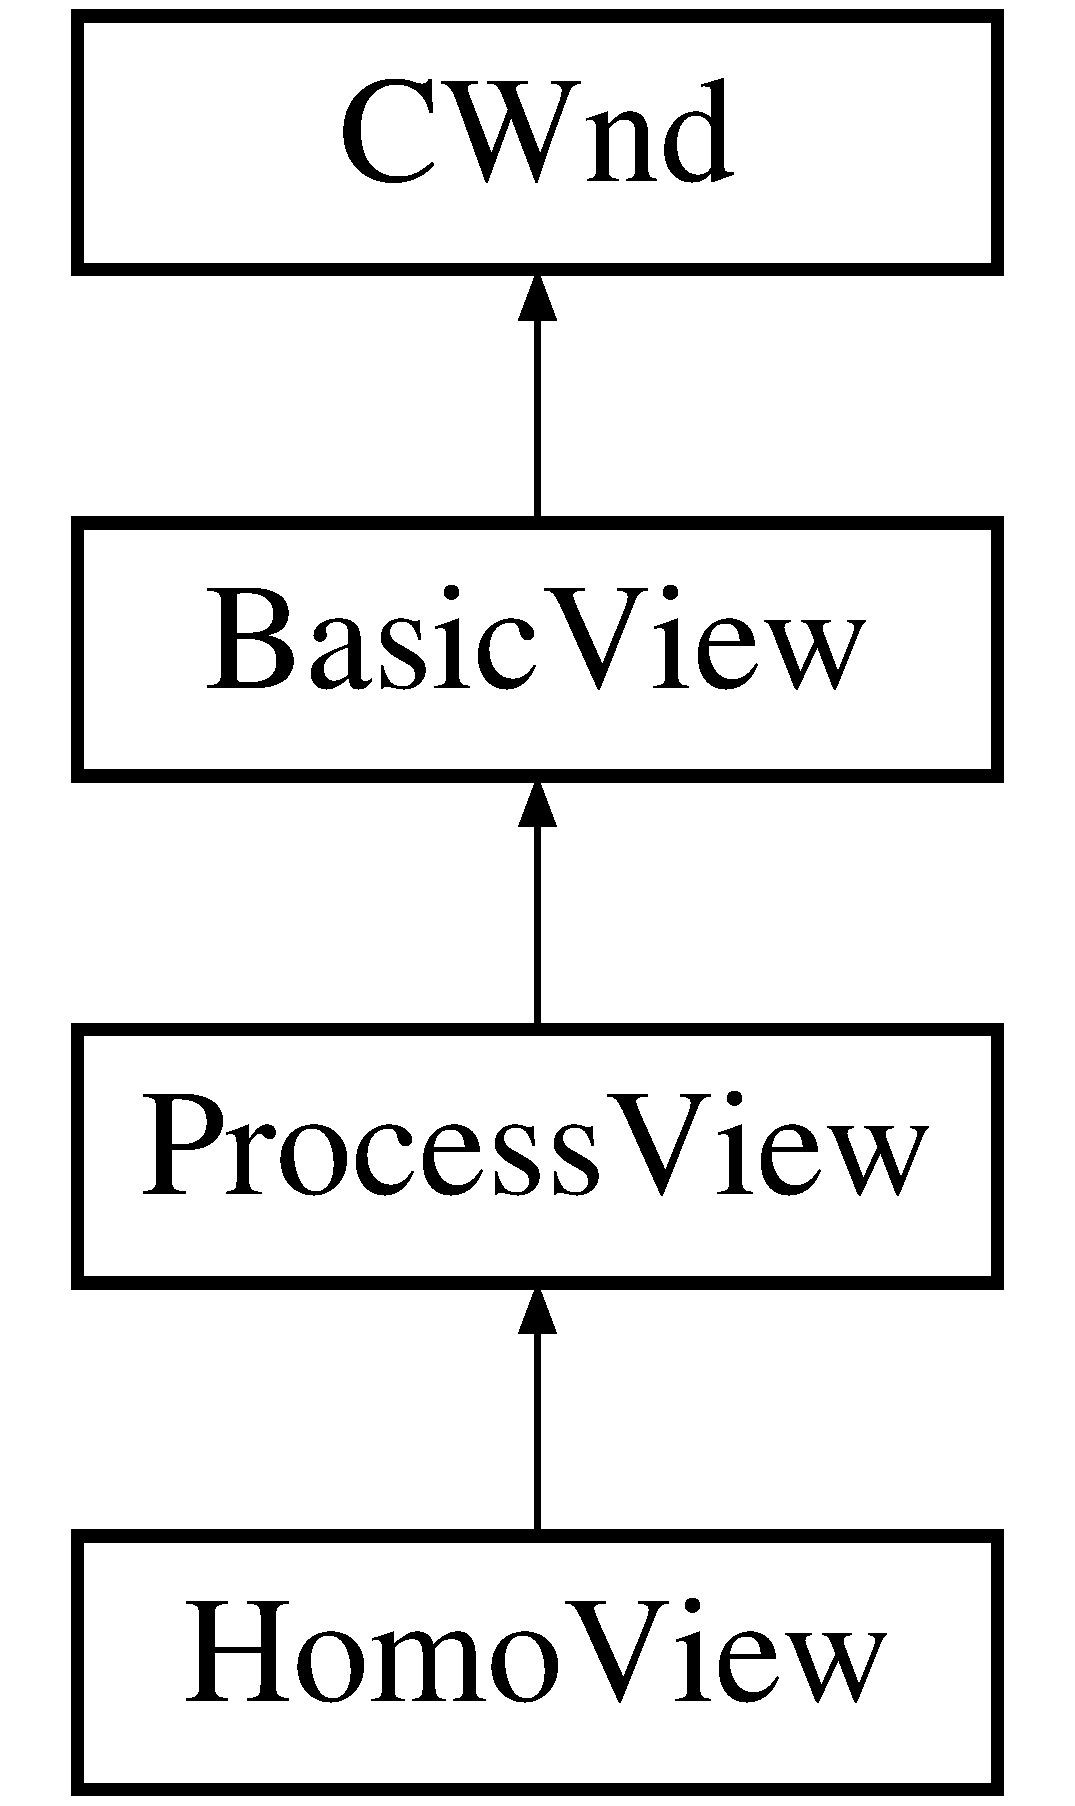
\includegraphics[height=4.000000cm]{class_homo_view}
\end{center}
\end{figure}
\subsection*{Public Member Functions}
\begin{DoxyCompactItemize}
\item 
\mbox{\Hypertarget{class_homo_view_a53f404f767b1fd329d07ad28a544c51e}\label{class_homo_view_a53f404f767b1fd329d07ad28a544c51e}} 
virtual void {\bfseries Set\+Param} (\mbox{\hyperlink{class_process_wrap}{Process\+Wrap}} $\ast$p\+Wrapper)
\item 
\mbox{\Hypertarget{class_homo_view_a216c8d44c93a078ef6ab750225d8fa79}\label{class_homo_view_a216c8d44c93a078ef6ab750225d8fa79}} 
afx\+\_\+msg void {\bfseries On\+Preview} ()
\end{DoxyCompactItemize}
\subsection*{Public Attributes}
\begin{DoxyCompactItemize}
\item 
\mbox{\Hypertarget{class_homo_view_a0eedb6c31537837e538865ce30c87645}\label{class_homo_view_a0eedb6c31537837e538865ce30c87645}} 
\mbox{\hyperlink{class_homo_wrap}{Homo\+Wrap}} $\ast$ {\bfseries m\+\_\+p\+Ldc\+Wrap}
\end{DoxyCompactItemize}
\subsection*{Protected Member Functions}
\begin{DoxyCompactItemize}
\item 
\mbox{\Hypertarget{class_homo_view_aaaa286aa764b94ccae653b34369a8036}\label{class_homo_view_aaaa286aa764b94ccae653b34369a8036}} 
virtual B\+O\+OL {\bfseries Pos\+Map} (int u, int v, float \&x, float \&y)
\item 
\mbox{\Hypertarget{class_homo_view_af79fa4c9d889d996557d6f9ee4979e6c}\label{class_homo_view_af79fa4c9d889d996557d6f9ee4979e6c}} 
virtual C\+O\+L\+O\+R\+R\+EF {\bfseries Get\+Color} (B\+Y\+TE $\ast$p\+Src, int stride, float x, float y)
\end{DoxyCompactItemize}
\subsection*{Additional Inherited Members}


\subsection{Detailed Description}
\mbox{\hyperlink{class_homo_view}{Homo\+View}} is the image viewer for Homography matrix processing image. It handles the video rendering process by the specified process. It is controlled by its process correspondent \mbox{\hyperlink{class_homo_tool}{Homo\+Tool}}. It also can display gride lines on the image window. 

\begin{DoxySeeAlso}{See also}
\mbox{\hyperlink{class_homo_tool}{Homo\+Tool}}. 
\end{DoxySeeAlso}


The documentation for this class was generated from the following files\+:\begin{DoxyCompactItemize}
\item 
i\+Optics/\mbox{\hyperlink{_homo_view_8h}{Homo\+View.\+h}}\item 
i\+Optics/Homo\+View.\+cpp\end{DoxyCompactItemize}

\hypertarget{class_homo_wrap}{}\section{Homo\+Wrap Class Reference}
\label{class_homo_wrap}\index{Homo\+Wrap@{Homo\+Wrap}}


Homogrphy matrix process parameters wrapper This class wrap Homography parameters and L\+UT table, as well as L\+UT generating function.  




{\ttfamily \#include $<$Homo\+Tool.\+h$>$}

Inheritance diagram for Homo\+Wrap\+:\begin{figure}[H]
\begin{center}
\leavevmode
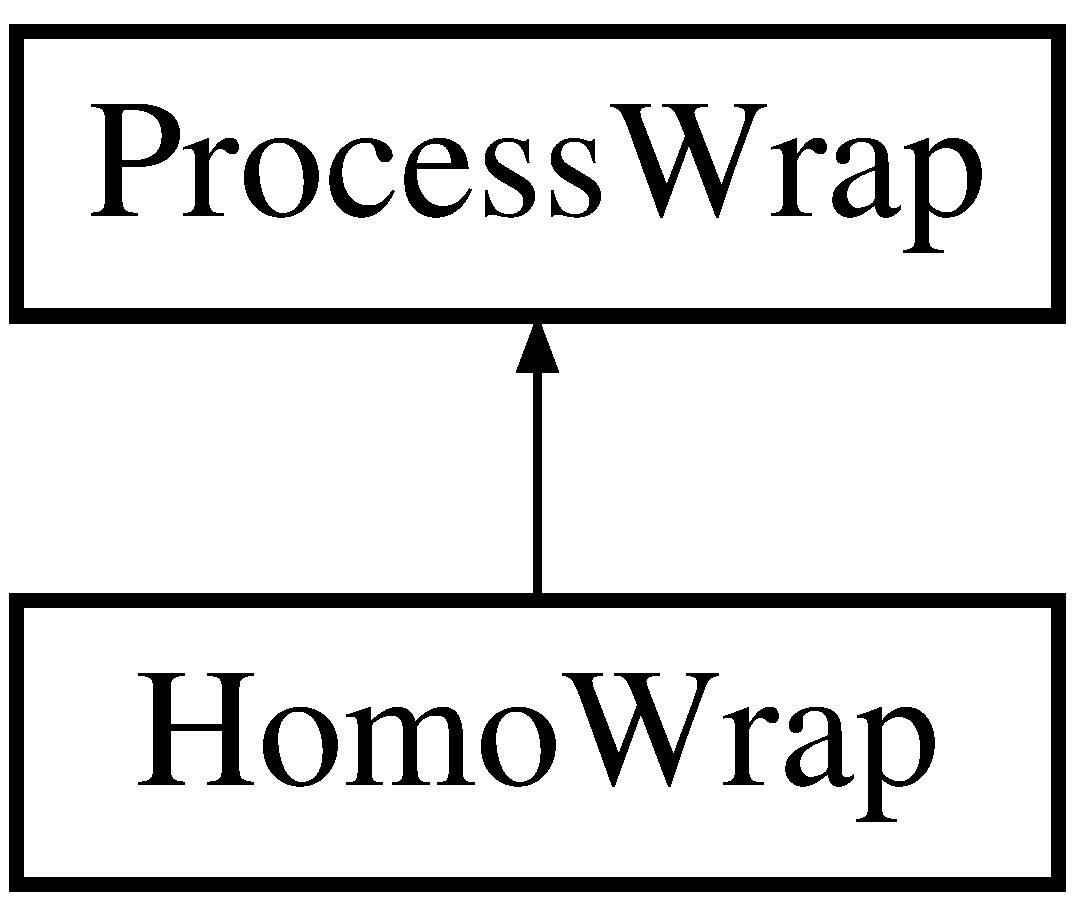
\includegraphics[height=2.000000cm]{class_homo_wrap}
\end{center}
\end{figure}
\subsection*{Public Member Functions}
\begin{DoxyCompactItemize}
\item 
virtual void \mbox{\hyperlink{class_homo_wrap_aecc7d5180e979679ad9e41ceaa846d05}{Set\+Param}} (void $\ast$p\+Param)
\item 
virtual void \mbox{\hyperlink{class_homo_wrap_a04c5506434d9afe322bfd6c08c51868f}{Make\+Map\+Table}} ()
\item 
virtual B\+O\+OL \mbox{\hyperlink{class_homo_wrap_a028ad1fea13805568dbe891f51dec7b2}{Pos\+Map}} (int u, int v, float \&x, float \&y)
\item 
virtual B\+O\+OL \mbox{\hyperlink{class_homo_wrap_aafd5595ef17a6be3074186204c39a550}{Save\+Parameter}} (L\+P\+C\+T\+S\+TR filename)
\item 
virtual B\+O\+OL \mbox{\hyperlink{class_homo_wrap_a5409cdfe65bc28ec3779f35eb3af22b4}{Load\+Parameter}} (L\+P\+C\+T\+S\+TR filename)
\end{DoxyCompactItemize}
\subsection*{Additional Inherited Members}


\subsection{Detailed Description}
Homogrphy matrix process parameters wrapper This class wrap Homography parameters and L\+UT table, as well as L\+UT generating function. 

\begin{DoxySeeAlso}{See also}
\mbox{\hyperlink{class_homo_view}{Homo\+View}} \mbox{\hyperlink{class_process_wrap}{Process\+Wrap}} 
\end{DoxySeeAlso}


\subsection{Member Function Documentation}
\mbox{\Hypertarget{class_homo_wrap_a5409cdfe65bc28ec3779f35eb3af22b4}\label{class_homo_wrap_a5409cdfe65bc28ec3779f35eb3af22b4}} 
\index{Homo\+Wrap@{Homo\+Wrap}!Load\+Parameter@{Load\+Parameter}}
\index{Load\+Parameter@{Load\+Parameter}!Homo\+Wrap@{Homo\+Wrap}}
\subsubsection{\texorpdfstring{Load\+Parameter()}{LoadParameter()}}
{\footnotesize\ttfamily virtual B\+O\+OL Load\+Parameter (\begin{DoxyParamCaption}\item[{L\+P\+C\+T\+S\+TR}]{filename }\end{DoxyParamCaption})\hspace{0.3cm}{\ttfamily [inline]}, {\ttfamily [virtual]}}

Read process specified parameters from a file. The format of data can be defined dependently by the correspondent \mbox{\hyperlink{class_process_wrap}{Process\+Wrap}} class. 

Implements \mbox{\hyperlink{class_process_wrap_a1cb75a423ff8f5ef736fc00a34792493}{Process\+Wrap}}.

\mbox{\Hypertarget{class_homo_wrap_a04c5506434d9afe322bfd6c08c51868f}\label{class_homo_wrap_a04c5506434d9afe322bfd6c08c51868f}} 
\index{Homo\+Wrap@{Homo\+Wrap}!Make\+Map\+Table@{Make\+Map\+Table}}
\index{Make\+Map\+Table@{Make\+Map\+Table}!Homo\+Wrap@{Homo\+Wrap}}
\subsubsection{\texorpdfstring{Make\+Map\+Table()}{MakeMapTable()}}
{\footnotesize\ttfamily virtual void Homo\+Wrap\+::\+Make\+Map\+Table (\begin{DoxyParamCaption}{ }\end{DoxyParamCaption})\hspace{0.3cm}{\ttfamily [inline]}, {\ttfamily [virtual]}}

Create the L\+UT data according the parameter 

Implements \mbox{\hyperlink{class_process_wrap_a22910a91f52147b8631b7e880509996e}{Process\+Wrap}}.

\mbox{\Hypertarget{class_homo_wrap_a028ad1fea13805568dbe891f51dec7b2}\label{class_homo_wrap_a028ad1fea13805568dbe891f51dec7b2}} 
\index{Homo\+Wrap@{Homo\+Wrap}!Pos\+Map@{Pos\+Map}}
\index{Pos\+Map@{Pos\+Map}!Homo\+Wrap@{Homo\+Wrap}}
\subsubsection{\texorpdfstring{Pos\+Map()}{PosMap()}}
{\footnotesize\ttfamily virtual B\+O\+OL Homo\+Wrap\+::\+Pos\+Map (\begin{DoxyParamCaption}\item[{int}]{u,  }\item[{int}]{v,  }\item[{float \&}]{x,  }\item[{float \&}]{y }\end{DoxyParamCaption})\hspace{0.3cm}{\ttfamily [inline]}, {\ttfamily [virtual]}}

Position mapping from processed image to original image 
\begin{DoxyParams}[1]{Parameters}
\mbox{\tt in}  & {\em u} & \mbox{[}0$\sim$sz\+Output.cx) in rocessed image \\
\hline
\mbox{\tt in}  & {\em v} & \mbox{[}0$\sim$sz\+Output.cy) in rocessed image \\
\hline
\mbox{\tt out}  & {\em x} & \mbox{[}0$\sim$sz\+Input.cx) in rocessed image \\
\hline
\mbox{\tt out}  & {\em y} & \mbox{[}0$\sim$sz\+Input.cy) in rocessed image \\
\hline
\end{DoxyParams}


Implements \mbox{\hyperlink{class_process_wrap_a536c940a16b6331109aa5d30763974fe}{Process\+Wrap}}.

\mbox{\Hypertarget{class_homo_wrap_aafd5595ef17a6be3074186204c39a550}\label{class_homo_wrap_aafd5595ef17a6be3074186204c39a550}} 
\index{Homo\+Wrap@{Homo\+Wrap}!Save\+Parameter@{Save\+Parameter}}
\index{Save\+Parameter@{Save\+Parameter}!Homo\+Wrap@{Homo\+Wrap}}
\subsubsection{\texorpdfstring{Save\+Parameter()}{SaveParameter()}}
{\footnotesize\ttfamily virtual B\+O\+OL Save\+Parameter (\begin{DoxyParamCaption}\item[{L\+P\+C\+T\+S\+TR}]{filename }\end{DoxyParamCaption})\hspace{0.3cm}{\ttfamily [inline]}, {\ttfamily [virtual]}}

Save process specified parameters in a file. The format of data can be defined dependently in this function. 

Implements \mbox{\hyperlink{class_process_wrap_aa5d4361a42a7a65cac877beb6d4ffa97}{Process\+Wrap}}.

\mbox{\Hypertarget{class_homo_wrap_aecc7d5180e979679ad9e41ceaa846d05}\label{class_homo_wrap_aecc7d5180e979679ad9e41ceaa846d05}} 
\index{Homo\+Wrap@{Homo\+Wrap}!Set\+Param@{Set\+Param}}
\index{Set\+Param@{Set\+Param}!Homo\+Wrap@{Homo\+Wrap}}
\subsubsection{\texorpdfstring{Set\+Param()}{SetParam()}}
{\footnotesize\ttfamily void Homo\+Wrap\+::\+Set\+Param (\begin{DoxyParamCaption}\item[{void $\ast$}]{p\+Param }\end{DoxyParamCaption})\hspace{0.3cm}{\ttfamily [virtual]}}

Sets Homography processing prameters, which is copied to class members and generate the L\+UT data. 
\begin{DoxyParams}{Parameters}
{\em p\+Param} & pointer to \\
\hline
\end{DoxyParams}


Reimplemented from \mbox{\hyperlink{class_process_wrap_a6c7130837d4713b0462f42cfc25aca98}{Process\+Wrap}}.



The documentation for this class was generated from the following files\+:\begin{DoxyCompactItemize}
\item 
i\+Optics/Homo\+Tool.\+h\item 
i\+Optics/Homo\+Tool.\+cpp\end{DoxyCompactItemize}

\hypertarget{class_ldc_tool}{}\section{Ldc\+Tool Class Reference}
\label{class_ldc_tool}\index{Ldc\+Tool@{Ldc\+Tool}}


Ldcc\+Tool is used to control the settings of Ldc process with UI in a dialog box. This class sends the parameters to a \mbox{\hyperlink{class_fec_view}{Fec\+View}} to display the resulted image. It also connects to a \mbox{\hyperlink{class_ldc_wrap}{Ldc\+Wrap}} class to maintain the L\+DC process related parameters and L\+UT data.  




{\ttfamily \#include $<$Ldc\+Tool.\+h$>$}

Inheritance diagram for Ldc\+Tool\+:\begin{figure}[H]
\begin{center}
\leavevmode
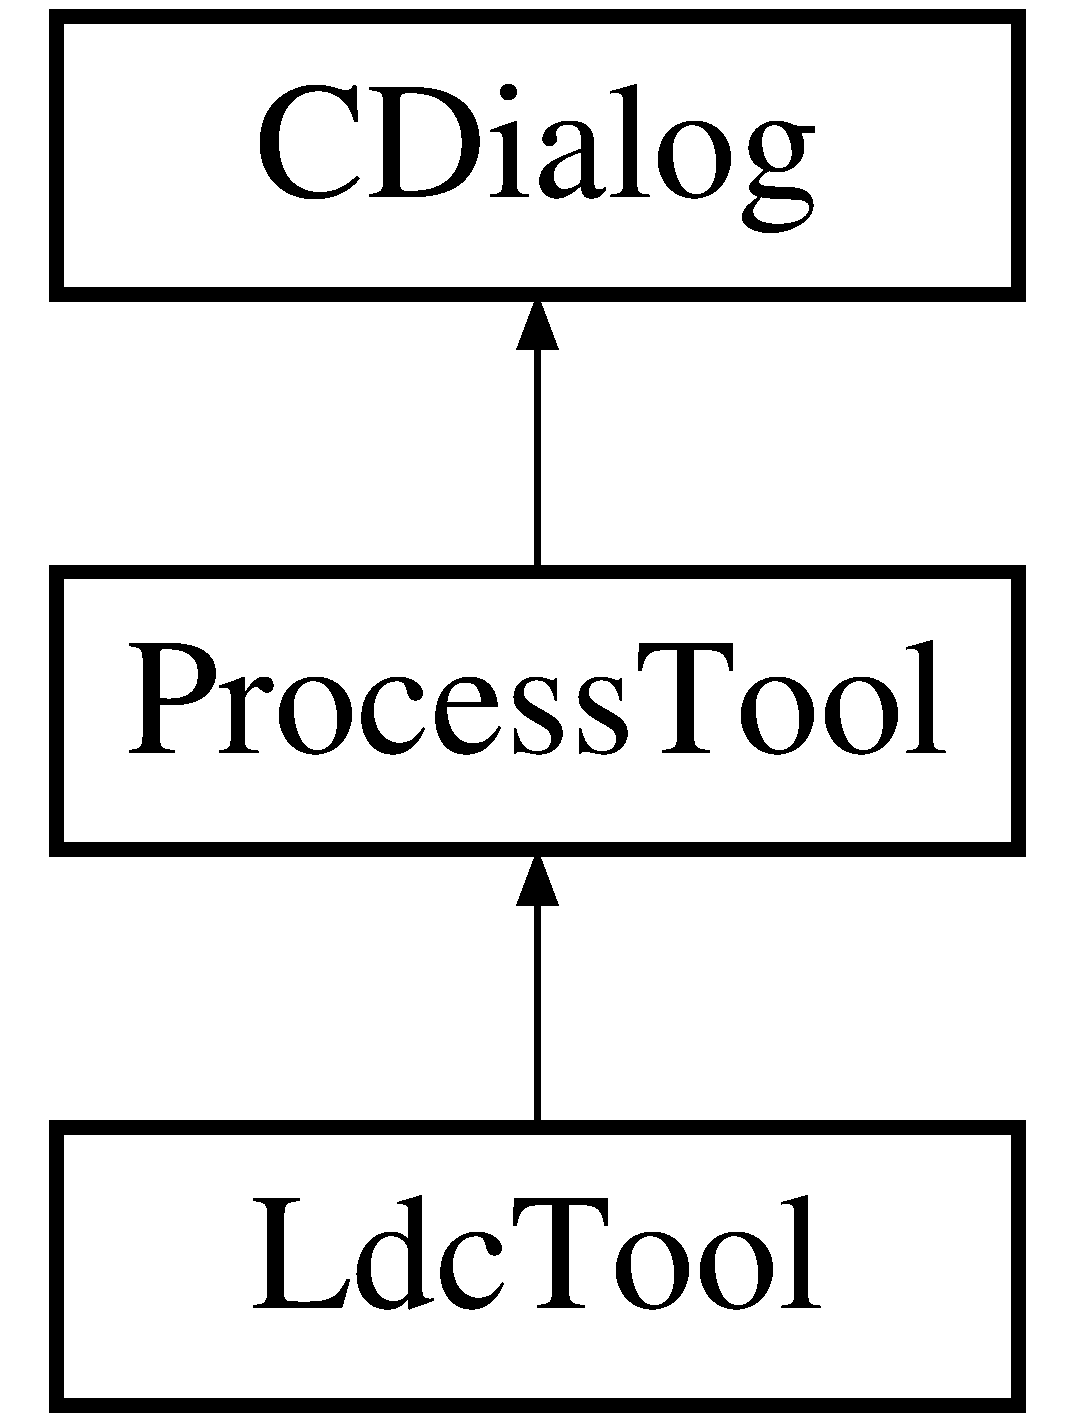
\includegraphics[height=3.000000cm]{class_ldc_tool}
\end{center}
\end{figure}
\subsection*{Public Types}
\begin{DoxyCompactItemize}
\item 
\mbox{\Hypertarget{class_ldc_tool_af2f77d69d4f8b26d5c400d16edbe88e1}\label{class_ldc_tool_af2f77d69d4f8b26d5c400d16edbe88e1}} 
enum \{ {\bfseries I\+DD} = I\+D\+D\+\_\+\+L\+DC
 \}
\end{DoxyCompactItemize}
\subsection*{Public Member Functions}
\begin{DoxyCompactItemize}
\item 
\mbox{\Hypertarget{class_ldc_tool_a136828a14c1f5cda892687c7b28ede87}\label{class_ldc_tool_a136828a14c1f5cda892687c7b28ede87}} 
{\bfseries Ldc\+Tool} (C\+Wnd $\ast$p\+Parent=N\+U\+LL)
\item 
virtual void \mbox{\hyperlink{class_ldc_tool_a1c98303e0ab2dfea1f1dcca8f1548307}{Set\+Param}} (\mbox{\hyperlink{class_process_wrap}{Process\+Wrap}} $\ast$p\+Param)
\item 
virtual \mbox{\hyperlink{class_process_wrap}{Process\+Wrap}} $\ast$ \mbox{\hyperlink{class_ldc_tool_af9828a2daf501b328a07dd8fa3d6abeb}{Get\+Param}} ()
\item 
virtual void \mbox{\hyperlink{class_ldc_tool_a07d1a547f02d4dea6a480c1be875a685}{Set\+Img\+File}} (Img\+File $\ast$p\+Image)
\end{DoxyCompactItemize}
\subsection*{Protected Member Functions}
\begin{DoxyCompactItemize}
\item 
\mbox{\Hypertarget{class_ldc_tool_a339d49ce8a034e52ed1dcfaf2a50b2d2}\label{class_ldc_tool_a339d49ce8a034e52ed1dcfaf2a50b2d2}} 
virtual void {\bfseries Do\+Data\+Exchange} (C\+Data\+Exchange $\ast$p\+DX)
\end{DoxyCompactItemize}
\subsection*{Additional Inherited Members}


\subsection{Detailed Description}
Ldcc\+Tool is used to control the settings of Ldc process with UI in a dialog box. This class sends the parameters to a \mbox{\hyperlink{class_fec_view}{Fec\+View}} to display the resulted image. It also connects to a \mbox{\hyperlink{class_ldc_wrap}{Ldc\+Wrap}} class to maintain the L\+DC process related parameters and L\+UT data. 

\subsection{Member Function Documentation}
\mbox{\Hypertarget{class_ldc_tool_af9828a2daf501b328a07dd8fa3d6abeb}\label{class_ldc_tool_af9828a2daf501b328a07dd8fa3d6abeb}} 
\index{Ldc\+Tool@{Ldc\+Tool}!Get\+Param@{Get\+Param}}
\index{Get\+Param@{Get\+Param}!Ldc\+Tool@{Ldc\+Tool}}
\subsubsection{\texorpdfstring{Get\+Param()}{GetParam()}}
{\footnotesize\ttfamily virtual \mbox{\hyperlink{class_process_wrap}{Process\+Wrap}}$\ast$ Ldc\+Tool\+::\+Get\+Param (\begin{DoxyParamCaption}{ }\end{DoxyParamCaption})\hspace{0.3cm}{\ttfamily [inline]}, {\ttfamily [virtual]}}

Gets the \mbox{\hyperlink{class_process_wrap}{Process\+Wrap}} class pointer of the process tool. 

Reimplemented from \mbox{\hyperlink{class_process_tool_a355ebcf991f86f59f4241ea4345547fc}{Process\+Tool}}.

\mbox{\Hypertarget{class_ldc_tool_a07d1a547f02d4dea6a480c1be875a685}\label{class_ldc_tool_a07d1a547f02d4dea6a480c1be875a685}} 
\index{Ldc\+Tool@{Ldc\+Tool}!Set\+Img\+File@{Set\+Img\+File}}
\index{Set\+Img\+File@{Set\+Img\+File}!Ldc\+Tool@{Ldc\+Tool}}
\subsubsection{\texorpdfstring{Set\+Img\+File()}{SetImgFile()}}
{\footnotesize\ttfamily void Ldc\+Tool\+::\+Set\+Img\+File (\begin{DoxyParamCaption}\item[{Img\+File $\ast$}]{p\+Image }\end{DoxyParamCaption})\hspace{0.3cm}{\ttfamily [virtual]}}

Sets the image to be processed from. The processed imaged won\textquotesingle{}t replace this original image. 

Reimplemented from \mbox{\hyperlink{class_process_tool_a178bc06abf5a20220bd2306a14708a93}{Process\+Tool}}.

\mbox{\Hypertarget{class_ldc_tool_a1c98303e0ab2dfea1f1dcca8f1548307}\label{class_ldc_tool_a1c98303e0ab2dfea1f1dcca8f1548307}} 
\index{Ldc\+Tool@{Ldc\+Tool}!Set\+Param@{Set\+Param}}
\index{Set\+Param@{Set\+Param}!Ldc\+Tool@{Ldc\+Tool}}
\subsubsection{\texorpdfstring{Set\+Param()}{SetParam()}}
{\footnotesize\ttfamily virtual void Ldc\+Tool\+::\+Set\+Param (\begin{DoxyParamCaption}\item[{\mbox{\hyperlink{class_process_wrap}{Process\+Wrap}} $\ast$}]{p\+Param }\end{DoxyParamCaption})\hspace{0.3cm}{\ttfamily [inline]}, {\ttfamily [virtual]}}

Copys contents of process parameters into related \mbox{\hyperlink{class_process_wrap}{Process\+Wrap}}. 

Reimplemented from \mbox{\hyperlink{class_process_tool_a50caa175198cece00b39a146715bf3eb}{Process\+Tool}}.



The documentation for this class was generated from the following files\+:\begin{DoxyCompactItemize}
\item 
i\+Optics/\mbox{\hyperlink{_ldc_tool_8h}{Ldc\+Tool.\+h}}\item 
i\+Optics/Ldc\+Tool.\+cpp\end{DoxyCompactItemize}

\hypertarget{class_ldc_view}{}\section{Ldc\+View Class Reference}
\label{class_ldc_view}\index{Ldc\+View@{Ldc\+View}}


\mbox{\hyperlink{class_ldc_view}{Ldc\+View}} is the image viewer for L\+DC processing image. It handles the video rendering process by the specified process. It is controlled by its process correspondent \mbox{\hyperlink{class_ldc_tool}{Ldc\+Tool}}. It also can display gride lines on the image window.  




{\ttfamily \#include $<$Ldc\+View.\+h$>$}

Inheritance diagram for Ldc\+View\+:\begin{figure}[H]
\begin{center}
\leavevmode
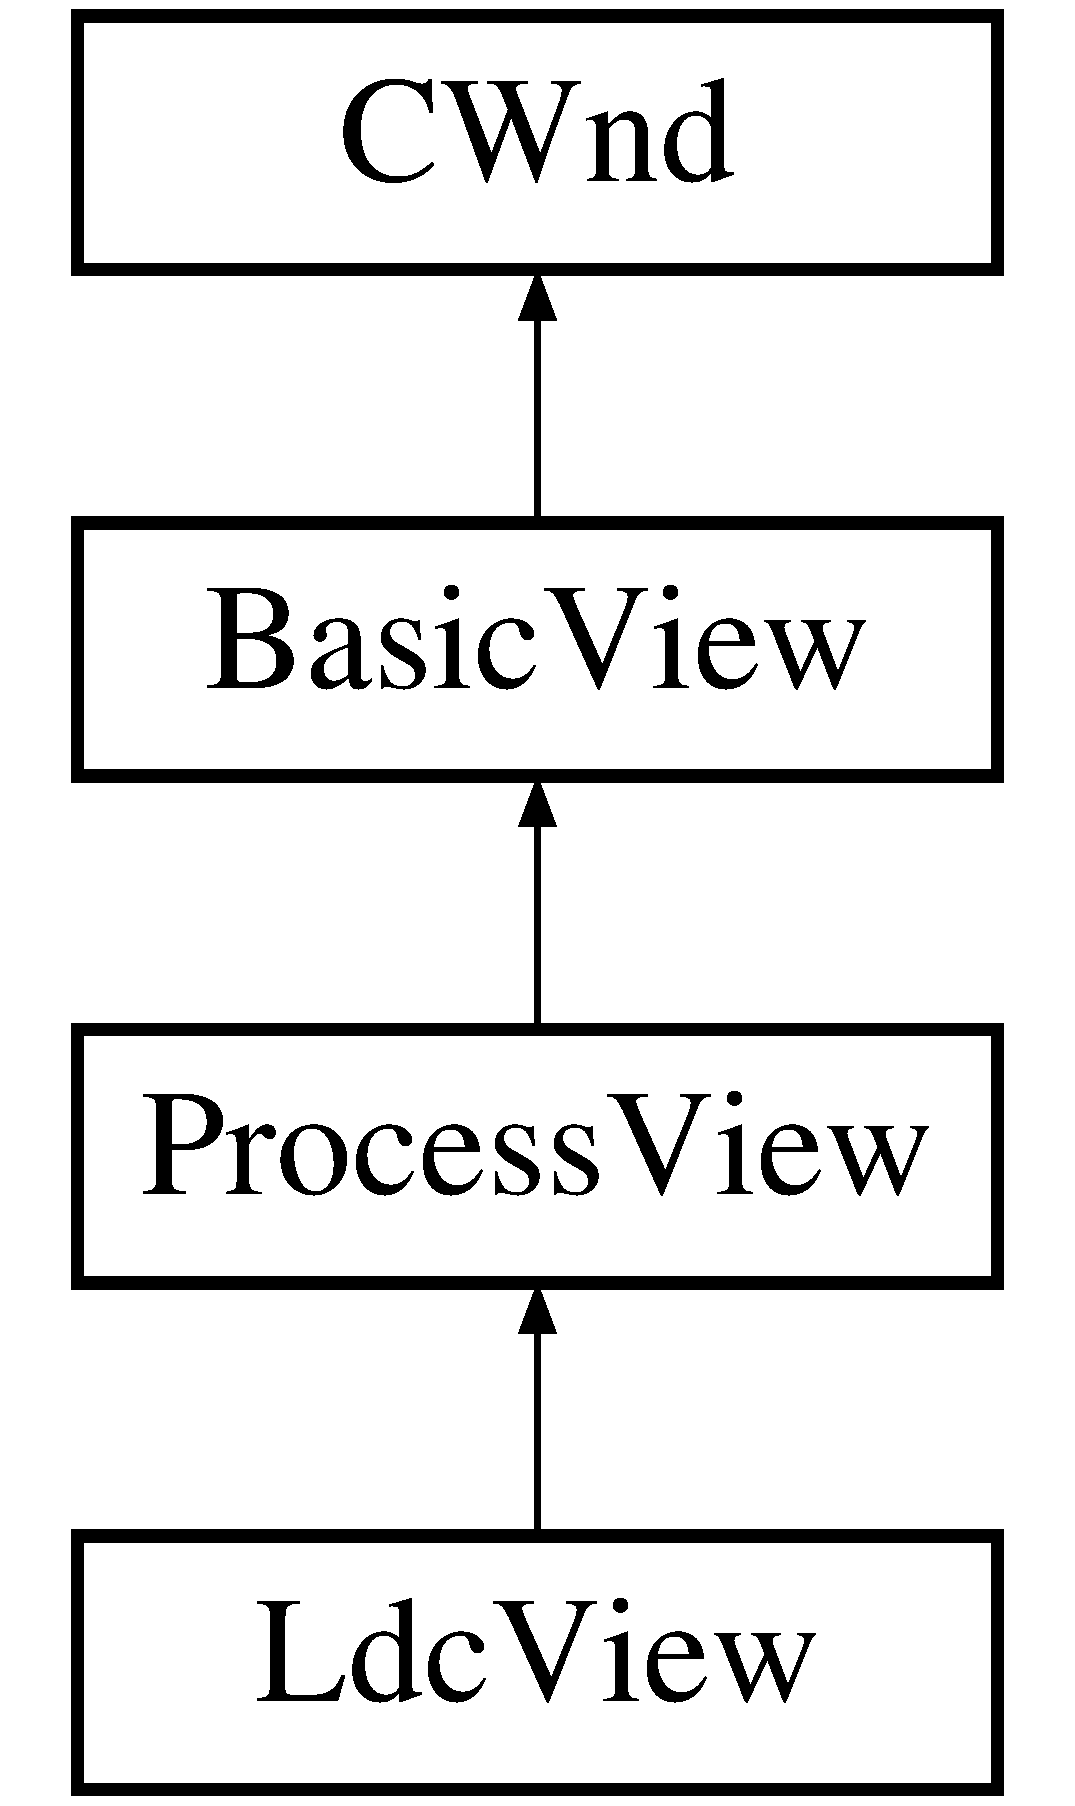
\includegraphics[height=4.000000cm]{class_ldc_view}
\end{center}
\end{figure}
\subsection*{Public Member Functions}
\begin{DoxyCompactItemize}
\item 
\mbox{\Hypertarget{class_ldc_view_a20c9c453f1e600fb26768d749276a85f}\label{class_ldc_view_a20c9c453f1e600fb26768d749276a85f}} 
virtual void {\bfseries Set\+Param} (\mbox{\hyperlink{class_process_wrap}{Process\+Wrap}} $\ast$p\+Wrapper)
\item 
\mbox{\Hypertarget{class_ldc_view_a5028dabeae808988f124ef5e79418c00}\label{class_ldc_view_a5028dabeae808988f124ef5e79418c00}} 
afx\+\_\+msg void {\bfseries On\+Preview} ()
\end{DoxyCompactItemize}
\subsection*{Public Attributes}
\begin{DoxyCompactItemize}
\item 
\mbox{\Hypertarget{class_ldc_view_aa6ebb786ca8301d34102439db0eca5e8}\label{class_ldc_view_aa6ebb786ca8301d34102439db0eca5e8}} 
\mbox{\hyperlink{class_ldc_wrap}{Ldc\+Wrap}} $\ast$ {\bfseries m\+\_\+p\+Ldc\+Wrap}
\end{DoxyCompactItemize}
\subsection*{Protected Member Functions}
\begin{DoxyCompactItemize}
\item 
\mbox{\Hypertarget{class_ldc_view_af6dc85960c6eb59a8b942fcbdcac287a}\label{class_ldc_view_af6dc85960c6eb59a8b942fcbdcac287a}} 
virtual B\+O\+OL {\bfseries Pos\+Map} (int u, int v, float \&x, float \&y)
\item 
\mbox{\Hypertarget{class_ldc_view_a5fff985c99999e4d012a0b8c3f15104c}\label{class_ldc_view_a5fff985c99999e4d012a0b8c3f15104c}} 
virtual C\+O\+L\+O\+R\+R\+EF {\bfseries Get\+Color} (B\+Y\+TE $\ast$p\+Src, int stride, float x, float y)
\end{DoxyCompactItemize}
\subsection*{Additional Inherited Members}


\subsection{Detailed Description}
\mbox{\hyperlink{class_ldc_view}{Ldc\+View}} is the image viewer for L\+DC processing image. It handles the video rendering process by the specified process. It is controlled by its process correspondent \mbox{\hyperlink{class_ldc_tool}{Ldc\+Tool}}. It also can display gride lines on the image window. 

\begin{DoxySeeAlso}{See also}
\mbox{\hyperlink{class_ldc_tool}{Ldc\+Tool}}. 
\end{DoxySeeAlso}


The documentation for this class was generated from the following files\+:\begin{DoxyCompactItemize}
\item 
i\+Optics/\mbox{\hyperlink{_ldc_view_8h}{Ldc\+View.\+h}}\item 
i\+Optics/Ldc\+View.\+cpp\end{DoxyCompactItemize}

\hypertarget{class_ldc_wrap}{}\section{Ldc\+Wrap Class Reference}
\label{class_ldc_wrap}\index{Ldc\+Wrap@{Ldc\+Wrap}}


L\+DC process parameters wrapper This class wrap L\+DC parameters and L\+UT table, as well as L\+UT generating function.  




{\ttfamily \#include $<$Ldc\+Tool.\+h$>$}

Inheritance diagram for Ldc\+Wrap\+:\begin{figure}[H]
\begin{center}
\leavevmode
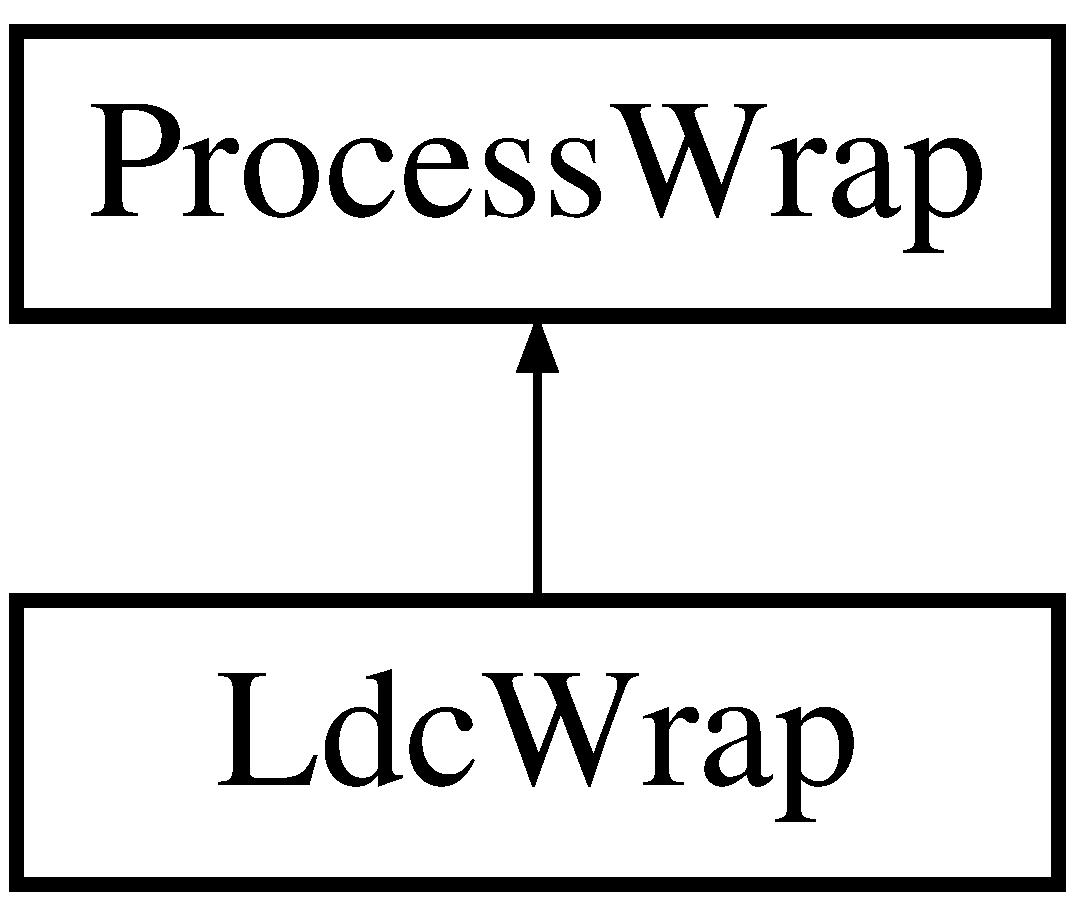
\includegraphics[height=2.000000cm]{class_ldc_wrap}
\end{center}
\end{figure}
\subsection*{Public Member Functions}
\begin{DoxyCompactItemize}
\item 
virtual void \mbox{\hyperlink{class_ldc_wrap_a0e99416d80b36d5da0faaa5a11da9ee7}{Set\+Param}} (void $\ast$p\+Param)
\item 
virtual void \mbox{\hyperlink{class_ldc_wrap_a0c6a77b5857bf0bc57c935b8612df9ad}{Make\+Map\+Table}} ()
\item 
virtual B\+O\+OL \mbox{\hyperlink{class_ldc_wrap_ad427e8c69a36be35bf5b95afa1d4fca3}{Pos\+Map}} (int u, int v, float \&x, float \&y)
\item 
virtual B\+O\+OL \mbox{\hyperlink{class_ldc_wrap_aafd5595ef17a6be3074186204c39a550}{Save\+Parameter}} (L\+P\+C\+T\+S\+TR filename)
\item 
virtual B\+O\+OL \mbox{\hyperlink{class_ldc_wrap_a5409cdfe65bc28ec3779f35eb3af22b4}{Load\+Parameter}} (L\+P\+C\+T\+S\+TR filename)
\end{DoxyCompactItemize}
\subsection*{Additional Inherited Members}


\subsection{Detailed Description}
L\+DC process parameters wrapper This class wrap L\+DC parameters and L\+UT table, as well as L\+UT generating function. 

\begin{DoxySeeAlso}{See also}
\mbox{\hyperlink{class_ldc_view}{Ldc\+View}} \mbox{\hyperlink{class_process_wrap}{Process\+Wrap}} 
\end{DoxySeeAlso}


\subsection{Member Function Documentation}
\mbox{\Hypertarget{class_ldc_wrap_a5409cdfe65bc28ec3779f35eb3af22b4}\label{class_ldc_wrap_a5409cdfe65bc28ec3779f35eb3af22b4}} 
\index{Ldc\+Wrap@{Ldc\+Wrap}!Load\+Parameter@{Load\+Parameter}}
\index{Load\+Parameter@{Load\+Parameter}!Ldc\+Wrap@{Ldc\+Wrap}}
\subsubsection{\texorpdfstring{Load\+Parameter()}{LoadParameter()}}
{\footnotesize\ttfamily virtual B\+O\+OL Load\+Parameter (\begin{DoxyParamCaption}\item[{L\+P\+C\+T\+S\+TR}]{filename }\end{DoxyParamCaption})\hspace{0.3cm}{\ttfamily [inline]}, {\ttfamily [virtual]}}

Read process specified parameters from a file. The format of data can be defined dependently by the correspondent \mbox{\hyperlink{class_process_wrap}{Process\+Wrap}} class. 

Implements \mbox{\hyperlink{class_process_wrap_a1cb75a423ff8f5ef736fc00a34792493}{Process\+Wrap}}.

\mbox{\Hypertarget{class_ldc_wrap_a0c6a77b5857bf0bc57c935b8612df9ad}\label{class_ldc_wrap_a0c6a77b5857bf0bc57c935b8612df9ad}} 
\index{Ldc\+Wrap@{Ldc\+Wrap}!Make\+Map\+Table@{Make\+Map\+Table}}
\index{Make\+Map\+Table@{Make\+Map\+Table}!Ldc\+Wrap@{Ldc\+Wrap}}
\subsubsection{\texorpdfstring{Make\+Map\+Table()}{MakeMapTable()}}
{\footnotesize\ttfamily virtual void Ldc\+Wrap\+::\+Make\+Map\+Table (\begin{DoxyParamCaption}{ }\end{DoxyParamCaption})\hspace{0.3cm}{\ttfamily [inline]}, {\ttfamily [virtual]}}

Create the L\+UT data according the parameter 

Implements \mbox{\hyperlink{class_process_wrap_a22910a91f52147b8631b7e880509996e}{Process\+Wrap}}.

\mbox{\Hypertarget{class_ldc_wrap_ad427e8c69a36be35bf5b95afa1d4fca3}\label{class_ldc_wrap_ad427e8c69a36be35bf5b95afa1d4fca3}} 
\index{Ldc\+Wrap@{Ldc\+Wrap}!Pos\+Map@{Pos\+Map}}
\index{Pos\+Map@{Pos\+Map}!Ldc\+Wrap@{Ldc\+Wrap}}
\subsubsection{\texorpdfstring{Pos\+Map()}{PosMap()}}
{\footnotesize\ttfamily virtual B\+O\+OL Ldc\+Wrap\+::\+Pos\+Map (\begin{DoxyParamCaption}\item[{int}]{u,  }\item[{int}]{v,  }\item[{float \&}]{x,  }\item[{float \&}]{y }\end{DoxyParamCaption})\hspace{0.3cm}{\ttfamily [inline]}, {\ttfamily [virtual]}}

Position mapping from processed image to original image 
\begin{DoxyParams}[1]{Parameters}
\mbox{\tt in}  & {\em u} & \mbox{[}0$\sim$sz\+Output.cx) in rocessed image \\
\hline
\mbox{\tt in}  & {\em v} & \mbox{[}0$\sim$sz\+Output.cy) in rocessed image \\
\hline
\mbox{\tt out}  & {\em x} & \mbox{[}0$\sim$sz\+Input.cx) in rocessed image \\
\hline
\mbox{\tt out}  & {\em y} & \mbox{[}0$\sim$sz\+Input.cy) in rocessed image \\
\hline
\end{DoxyParams}


Implements \mbox{\hyperlink{class_process_wrap_a536c940a16b6331109aa5d30763974fe}{Process\+Wrap}}.

\mbox{\Hypertarget{class_ldc_wrap_aafd5595ef17a6be3074186204c39a550}\label{class_ldc_wrap_aafd5595ef17a6be3074186204c39a550}} 
\index{Ldc\+Wrap@{Ldc\+Wrap}!Save\+Parameter@{Save\+Parameter}}
\index{Save\+Parameter@{Save\+Parameter}!Ldc\+Wrap@{Ldc\+Wrap}}
\subsubsection{\texorpdfstring{Save\+Parameter()}{SaveParameter()}}
{\footnotesize\ttfamily virtual B\+O\+OL Save\+Parameter (\begin{DoxyParamCaption}\item[{L\+P\+C\+T\+S\+TR}]{filename }\end{DoxyParamCaption})\hspace{0.3cm}{\ttfamily [inline]}, {\ttfamily [virtual]}}

Save process specified parameters in a file. The format of data can be defined dependently in this function. 

Implements \mbox{\hyperlink{class_process_wrap_aa5d4361a42a7a65cac877beb6d4ffa97}{Process\+Wrap}}.

\mbox{\Hypertarget{class_ldc_wrap_a0e99416d80b36d5da0faaa5a11da9ee7}\label{class_ldc_wrap_a0e99416d80b36d5da0faaa5a11da9ee7}} 
\index{Ldc\+Wrap@{Ldc\+Wrap}!Set\+Param@{Set\+Param}}
\index{Set\+Param@{Set\+Param}!Ldc\+Wrap@{Ldc\+Wrap}}
\subsubsection{\texorpdfstring{Set\+Param()}{SetParam()}}
{\footnotesize\ttfamily void Ldc\+Wrap\+::\+Set\+Param (\begin{DoxyParamCaption}\item[{void $\ast$}]{p\+Param }\end{DoxyParamCaption})\hspace{0.3cm}{\ttfamily [virtual]}}

Sets L\+DC processing prameters, which is copied to class members and generate the L\+UT data. 
\begin{DoxyParams}{Parameters}
{\em p\+Param} & pointer to m\+\_\+db\+Coef. \\
\hline
\end{DoxyParams}


Reimplemented from \mbox{\hyperlink{class_process_wrap_a6c7130837d4713b0462f42cfc25aca98}{Process\+Wrap}}.



The documentation for this class was generated from the following files\+:\begin{DoxyCompactItemize}
\item 
i\+Optics/\mbox{\hyperlink{_ldc_tool_8h}{Ldc\+Tool.\+h}}\item 
i\+Optics/Ldc\+Tool.\+cpp\end{DoxyCompactItemize}

\hypertarget{class_measure_performance}{}\section{Measure\+Performance Class Reference}
\label{class_measure_performance}\index{Measure\+Performance@{Measure\+Performance}}
\subsection*{Public Member Functions}
\begin{DoxyCompactItemize}
\item 
\mbox{\Hypertarget{class_measure_performance_ad96801923dd8aa96e23077ae83f33a33}\label{class_measure_performance_ad96801923dd8aa96e23077ae83f33a33}} 
void {\bfseries start} ()
\item 
\mbox{\Hypertarget{class_measure_performance_abf56a715d5664ea3337d2a7271c3f061}\label{class_measure_performance_abf56a715d5664ea3337d2a7271c3f061}} 
void {\bfseries end} ()
\item 
\mbox{\Hypertarget{class_measure_performance_af26500cfebbec5fd006be3c5089100c4}\label{class_measure_performance_af26500cfebbec5fd006be3c5089100c4}} 
void {\bfseries resume} ()
\item 
\mbox{\Hypertarget{class_measure_performance_aa3b5b93a1b5faeb7d0a6533cd964bfd7}\label{class_measure_performance_aa3b5b93a1b5faeb7d0a6533cd964bfd7}} 
double {\bfseries duration} ()
\end{DoxyCompactItemize}


The documentation for this class was generated from the following files\+:\begin{DoxyCompactItemize}
\item 
i\+Optics/Measure\+Performance.\+h\item 
i\+Optics/Measure\+Performance.\+cpp\end{DoxyCompactItemize}

\hypertarget{class_mesh}{}\section{Mesh Class Reference}
\label{class_mesh}\index{Mesh@{Mesh}}


Draw mesh on the specified area working flow.  




{\ttfamily \#include $<$Mesh.\+h$>$}

\subsection*{Public Member Functions}
\begin{DoxyCompactItemize}
\item 
B\+O\+OL \mbox{\hyperlink{class_mesh_a79aa8ef87d68988f999a00bfea114632}{Set\+Table}} (\mbox{\hyperlink{struct___point_double}{Point\+Double}} $\ast$p\+Lut, int column, int row)
\item 
void \mbox{\hyperlink{class_mesh_a2c9670a5720afe8ee5bcaa6c433455d5}{Release}} ()
\item 
void \mbox{\hyperlink{class_mesh_a28a00f1a751e2a5cca3425670befc376}{Set\+Location\+On\+Canvas}} (R\+E\+CT \&rc\+Location)
\item 
void \mbox{\hyperlink{class_mesh_ab55d4ba1fb6a9e49651dc4801392df6d}{Draw}} (C\+DC $\ast$p\+DC, R\+E\+CT $\ast$p\+View\+Port, B\+O\+OL b\+Show\+All)
\item 
void \mbox{\hyperlink{class_mesh_a40ac4b15e3c738aab4c701d774e65ce9}{Move\+Control\+Point}} (int m, int n, P\+O\+I\+NT offset)
\item 
B\+O\+OL \mbox{\hyperlink{class_mesh_a945caa648924bf3336a54c075b83e019}{Is\+On\+Control\+Point}} (P\+O\+I\+NT pt\+Cursor, P\+O\+I\+NT \&index)
\item 
void \mbox{\hyperlink{class_mesh_ad644e7f3d14e64774bc32c356898109c}{On\+Mouse\+Move}} (C\+Wnd $\ast$p\+Wnd, P\+O\+I\+NT pos)
\item 
\mbox{\Hypertarget{class_mesh_af80676782b87f7a31b7c8d6d0fbe29af}\label{class_mesh_af80676782b87f7a31b7c8d6d0fbe29af}} 
void {\bfseries On\+L\+Button\+Down} (C\+Wnd $\ast$p\+Wnd, P\+O\+I\+NT pos)
\item 
\mbox{\Hypertarget{class_mesh_a7cd53f709a59db03c99998e0402e9852}\label{class_mesh_a7cd53f709a59db03c99998e0402e9852}} 
void {\bfseries On\+L\+Button\+Up} (C\+Wnd $\ast$p\+Wnd, P\+O\+I\+NT pos)
\end{DoxyCompactItemize}


\subsection{Detailed Description}
Draw mesh on the specified area working flow. 


\begin{DoxyImageNoCaption}
  \mbox{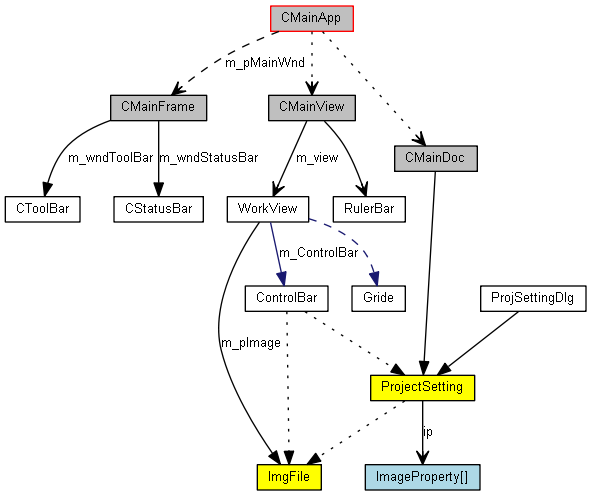
\includegraphics[width=\textwidth,height=\textheight/2,keepaspectratio=true]{dot_inline_dotgraph_1}}
\end{DoxyImageNoCaption}
 

\subsection{Member Function Documentation}
\mbox{\Hypertarget{class_mesh_ab55d4ba1fb6a9e49651dc4801392df6d}\label{class_mesh_ab55d4ba1fb6a9e49651dc4801392df6d}} 
\index{Mesh@{Mesh}!Draw@{Draw}}
\index{Draw@{Draw}!Mesh@{Mesh}}
\subsubsection{\texorpdfstring{Draw()}{Draw()}}
{\footnotesize\ttfamily void Mesh\+::\+Draw (\begin{DoxyParamCaption}\item[{C\+DC $\ast$}]{p\+DC,  }\item[{R\+E\+CT $\ast$}]{p\+View\+Port,  }\item[{B\+O\+OL}]{b\+Show\+All }\end{DoxyParamCaption})}

Display mesh within rc\+View\+Port, show Control point only if b\+Show\+All is F\+A\+L\+SE \mbox{\Hypertarget{class_mesh_a945caa648924bf3336a54c075b83e019}\label{class_mesh_a945caa648924bf3336a54c075b83e019}} 
\index{Mesh@{Mesh}!Is\+On\+Control\+Point@{Is\+On\+Control\+Point}}
\index{Is\+On\+Control\+Point@{Is\+On\+Control\+Point}!Mesh@{Mesh}}
\subsubsection{\texorpdfstring{Is\+On\+Control\+Point()}{IsOnControlPoint()}}
{\footnotesize\ttfamily B\+O\+OL Mesh\+::\+Is\+On\+Control\+Point (\begin{DoxyParamCaption}\item[{P\+O\+I\+NT}]{pt\+Cursor,  }\item[{P\+O\+I\+NT \&}]{index }\end{DoxyParamCaption})}

Check if pt\+Cursor (canvas coordinate) is on a control point if return T\+R\+UE, CP index is write tp index Display mesh within rc\+View\+Port, show Control point only if b\+Show\+All is F\+A\+L\+SE \mbox{\Hypertarget{class_mesh_a40ac4b15e3c738aab4c701d774e65ce9}\label{class_mesh_a40ac4b15e3c738aab4c701d774e65ce9}} 
\index{Mesh@{Mesh}!Move\+Control\+Point@{Move\+Control\+Point}}
\index{Move\+Control\+Point@{Move\+Control\+Point}!Mesh@{Mesh}}
\subsubsection{\texorpdfstring{Move\+Control\+Point()}{MoveControlPoint()}}
{\footnotesize\ttfamily void Mesh\+::\+Move\+Control\+Point (\begin{DoxyParamCaption}\item[{int}]{m,  }\item[{int}]{n,  }\item[{P\+O\+I\+NT}]{offset }\end{DoxyParamCaption})}

Move indexed control point by offset with real world coordinates \mbox{\Hypertarget{class_mesh_ad644e7f3d14e64774bc32c356898109c}\label{class_mesh_ad644e7f3d14e64774bc32c356898109c}} 
\index{Mesh@{Mesh}!On\+Mouse\+Move@{On\+Mouse\+Move}}
\index{On\+Mouse\+Move@{On\+Mouse\+Move}!Mesh@{Mesh}}
\subsubsection{\texorpdfstring{On\+Mouse\+Move()}{OnMouseMove()}}
{\footnotesize\ttfamily void Mesh\+::\+On\+Mouse\+Move (\begin{DoxyParamCaption}\item[{C\+Wnd $\ast$}]{p\+Wnd,  }\item[{P\+O\+I\+NT}]{pos }\end{DoxyParamCaption})}

Mouse event handling. pos is Canvas coordinate. \mbox{\Hypertarget{class_mesh_a2c9670a5720afe8ee5bcaa6c433455d5}\label{class_mesh_a2c9670a5720afe8ee5bcaa6c433455d5}} 
\index{Mesh@{Mesh}!Release@{Release}}
\index{Release@{Release}!Mesh@{Mesh}}
\subsubsection{\texorpdfstring{Release()}{Release()}}
{\footnotesize\ttfamily void Mesh\+::\+Release (\begin{DoxyParamCaption}{ }\end{DoxyParamCaption})}

Clears all resource. \mbox{\Hypertarget{class_mesh_a28a00f1a751e2a5cca3425670befc376}\label{class_mesh_a28a00f1a751e2a5cca3425670befc376}} 
\index{Mesh@{Mesh}!Set\+Location\+On\+Canvas@{Set\+Location\+On\+Canvas}}
\index{Set\+Location\+On\+Canvas@{Set\+Location\+On\+Canvas}!Mesh@{Mesh}}
\subsubsection{\texorpdfstring{Set\+Location\+On\+Canvas()}{SetLocationOnCanvas()}}
{\footnotesize\ttfamily void Mesh\+::\+Set\+Location\+On\+Canvas (\begin{DoxyParamCaption}\item[{R\+E\+CT \&}]{rc\+Location }\end{DoxyParamCaption})}

Remap mesh to real world coordinates \mbox{\Hypertarget{class_mesh_a79aa8ef87d68988f999a00bfea114632}\label{class_mesh_a79aa8ef87d68988f999a00bfea114632}} 
\index{Mesh@{Mesh}!Set\+Table@{Set\+Table}}
\index{Set\+Table@{Set\+Table}!Mesh@{Mesh}}
\subsubsection{\texorpdfstring{Set\+Table()}{SetTable()}}
{\footnotesize\ttfamily B\+O\+OL Mesh\+::\+Set\+Table (\begin{DoxyParamCaption}\item[{\mbox{\hyperlink{struct___point_double}{Point\+Double}} $\ast$}]{p\+Lut,  }\item[{int}]{column,  }\item[{int}]{row }\end{DoxyParamCaption})}

Sets the L\+UT data and specify its dimension. this function is called when content of table is changed 
\begin{DoxyParams}[1]{Parameters}
\mbox{\tt in}  & {\em p\+Lut} & L\+UT contents to set. If p\+Lut != N\+U\+LL, copy p\+Lut to p\+Cp, else makes p\+Cp as rectangle grides \\
\hline
\mbox{\tt in}  & {\em column} & numbers of vertical lines, including border \\
\hline
\mbox{\tt in}  & {\em row} & numbers of horizontal lines, including border \\
\hline
\end{DoxyParams}
\begin{DoxyReturn}{Returns}
F\+A\+L\+SE if failed to allocat internal L\+UT memory. 
\end{DoxyReturn}


The documentation for this class was generated from the following files\+:\begin{DoxyCompactItemize}
\item 
i\+Optics/\mbox{\hyperlink{_mesh_8h}{Mesh.\+h}}\item 
i\+Optics/\mbox{\hyperlink{_mesh_8cpp}{Mesh.\+cpp}}\end{DoxyCompactItemize}

\hypertarget{class_navigator}{}\section{Navigator Class Reference}
\label{class_navigator}\index{Navigator@{Navigator}}
Inheritance diagram for Navigator\+:\begin{figure}[H]
\begin{center}
\leavevmode
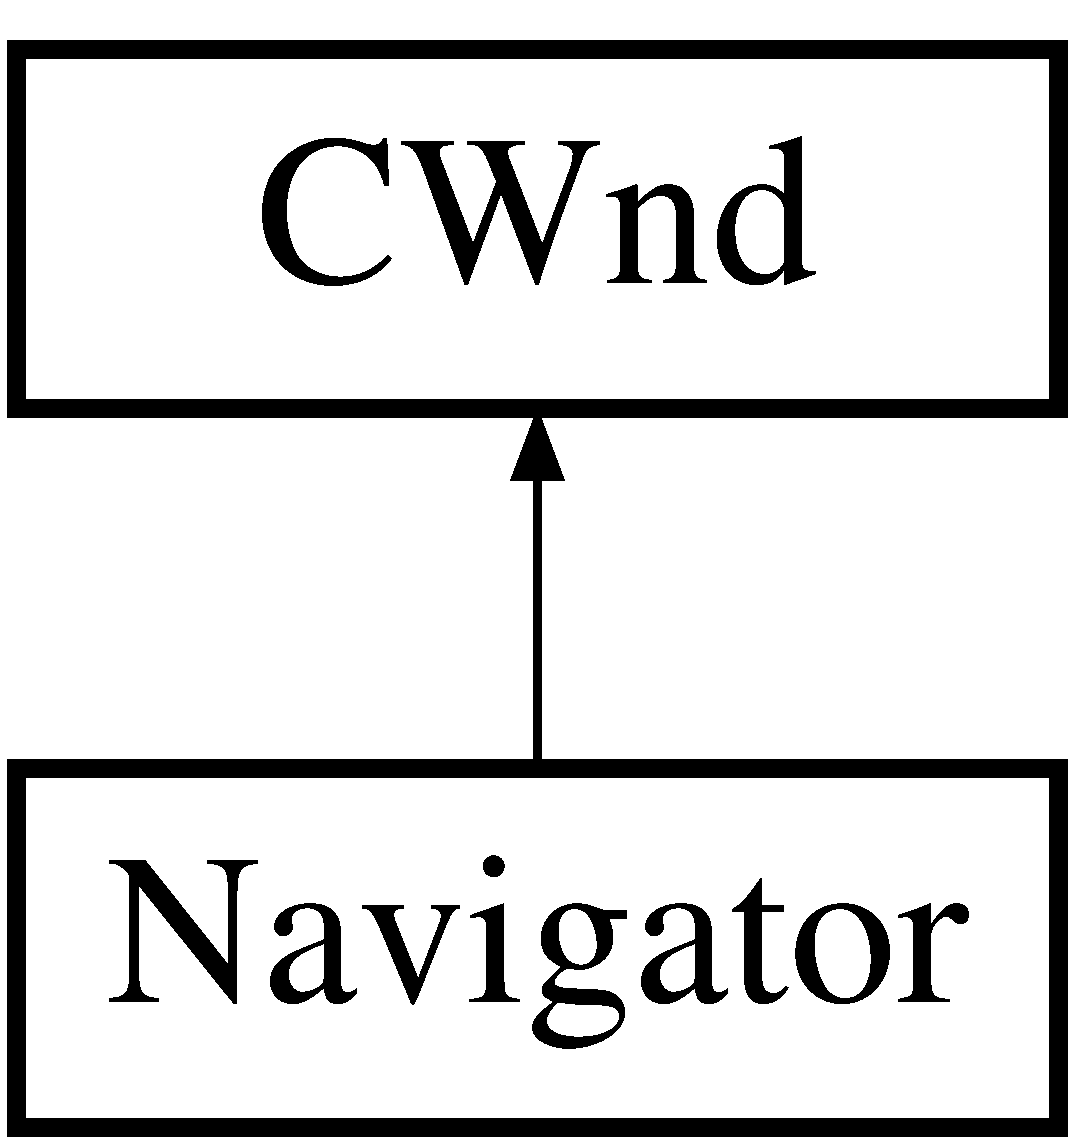
\includegraphics[height=2.000000cm]{class_navigator}
\end{center}
\end{figure}
\subsection*{Public Member Functions}
\begin{DoxyCompactItemize}
\item 
\mbox{\Hypertarget{class_navigator_a9d42cf2b335c6366f4f70c09a07c31c0}\label{class_navigator_a9d42cf2b335c6366f4f70c09a07c31c0}} 
virtual B\+O\+OL {\bfseries Create} (L\+P\+C\+T\+S\+TR lpsz\+Class\+Name, L\+P\+C\+T\+S\+TR lpsz\+Window\+Name, D\+W\+O\+RD dw\+Style, const R\+E\+CT \&rect, C\+Wnd $\ast$p\+Parent\+Wnd, U\+I\+NT n\+ID, C\+Create\+Context $\ast$p\+Context=N\+U\+LL)
\item 
\mbox{\Hypertarget{class_navigator_aa7ba51bbca8910888f8a72c2c3948955}\label{class_navigator_aa7ba51bbca8910888f8a72c2c3948955}} 
B\+O\+OL {\bfseries Set\+Image} (Img\+File $\ast$p\+Dib)
\item 
\mbox{\Hypertarget{class_navigator_a859cb322ac1f07a22ad361098bfacc1c}\label{class_navigator_a859cb322ac1f07a22ad361098bfacc1c}} 
B\+O\+OL {\bfseries Create} (C\+Wnd $\ast$p\+Wnd, int x, int y)
\end{DoxyCompactItemize}
\subsection*{Public Attributes}
\begin{DoxyCompactItemize}
\item 
\mbox{\Hypertarget{class_navigator_a242d4351f7c96e1269e172086fb44e01}\label{class_navigator_a242d4351f7c96e1269e172086fb44e01}} 
C\+Rect {\bfseries m\+\_\+rc\+Img}
\end{DoxyCompactItemize}
\subsection*{Protected Member Functions}
\begin{DoxyCompactItemize}
\item 
\mbox{\Hypertarget{class_navigator_abed125f064d55901ab7037d16414ff3d}\label{class_navigator_abed125f064d55901ab7037d16414ff3d}} 
afx\+\_\+msg void {\bfseries On\+Destroy} ()
\item 
\mbox{\Hypertarget{class_navigator_a03c00a5cff644d9130c79d2ac1c0a477}\label{class_navigator_a03c00a5cff644d9130c79d2ac1c0a477}} 
afx\+\_\+msg void {\bfseries On\+Paint} ()
\item 
\mbox{\Hypertarget{class_navigator_a06ef074cb12d849045cda801542f5324}\label{class_navigator_a06ef074cb12d849045cda801542f5324}} 
afx\+\_\+msg void {\bfseries On\+L\+Button\+Down} (U\+I\+NT n\+Flags, C\+Point point)
\item 
\mbox{\Hypertarget{class_navigator_a928fb26ee69a9055abfaec5be4aafba2}\label{class_navigator_a928fb26ee69a9055abfaec5be4aafba2}} 
afx\+\_\+msg void {\bfseries On\+L\+Button\+Up} (U\+I\+NT n\+Flags, C\+Point point)
\item 
\mbox{\Hypertarget{class_navigator_ac22c3de57fe917db53d9d39f1f73332a}\label{class_navigator_ac22c3de57fe917db53d9d39f1f73332a}} 
afx\+\_\+msg void {\bfseries On\+Mouse\+Move} (U\+I\+NT n\+Flags, C\+Point point)
\item 
\mbox{\Hypertarget{class_navigator_a02c933f968cd19da2543e74950cfd3e4}\label{class_navigator_a02c933f968cd19da2543e74950cfd3e4}} 
afx\+\_\+msg B\+O\+OL {\bfseries On\+Mouse\+Wheel} (U\+I\+NT n\+Flags, short z\+Delta, C\+Point pt)
\item 
\mbox{\Hypertarget{class_navigator_a2f96fee841493e852cdeecc32889aa3a}\label{class_navigator_a2f96fee841493e852cdeecc32889aa3a}} 
afx\+\_\+msg B\+O\+OL {\bfseries On\+Erase\+Bkgnd} (C\+DC $\ast$p\+DC)
\end{DoxyCompactItemize}
\subsection*{Protected Attributes}
\begin{DoxyCompactItemize}
\item 
\mbox{\Hypertarget{class_navigator_aa042070b419a6b78a71107cc927494b2}\label{class_navigator_aa042070b419a6b78a71107cc927494b2}} 
\mbox{\hyperlink{class_c_main_view}{C\+Main\+View}} $\ast$ {\bfseries m\+\_\+p\+Parent}
\end{DoxyCompactItemize}


The documentation for this class was generated from the following files\+:\begin{DoxyCompactItemize}
\item 
i\+Optics/Navigator.\+h\item 
i\+Optics/Navigator.\+cpp\end{DoxyCompactItemize}

\hypertarget{class_process_tool}{}\section{Process\+Tool Class Reference}
\label{class_process_tool}\index{Process\+Tool@{Process\+Tool}}


\mbox{\hyperlink{class_process_tool}{Process\+Tool}} is the abstract class which is used to control the settings of a process with UI in a dialog box. A \mbox{\hyperlink{class_process_tool}{Process\+Tool}} class consistent of a \mbox{\hyperlink{class_process_view}{Process\+View}} member to display the processed image and a \mbox{\hyperlink{class_process_wrap}{Process\+Wrap}} class member to aintain the process related parameters and L\+UT data. \mbox{\hyperlink{class_process_tool}{Process\+Tool}} is the bridge class between \mbox{\hyperlink{class_work_view}{Work\+View}} and the Process. The application use \mbox{\hyperlink{class_process_tool}{Process\+Tool}} to access the specified process stuff.  




{\ttfamily \#include $<$Process\+Tool.\+h$>$}

Inheritance diagram for Process\+Tool\+:\begin{figure}[H]
\begin{center}
\leavevmode
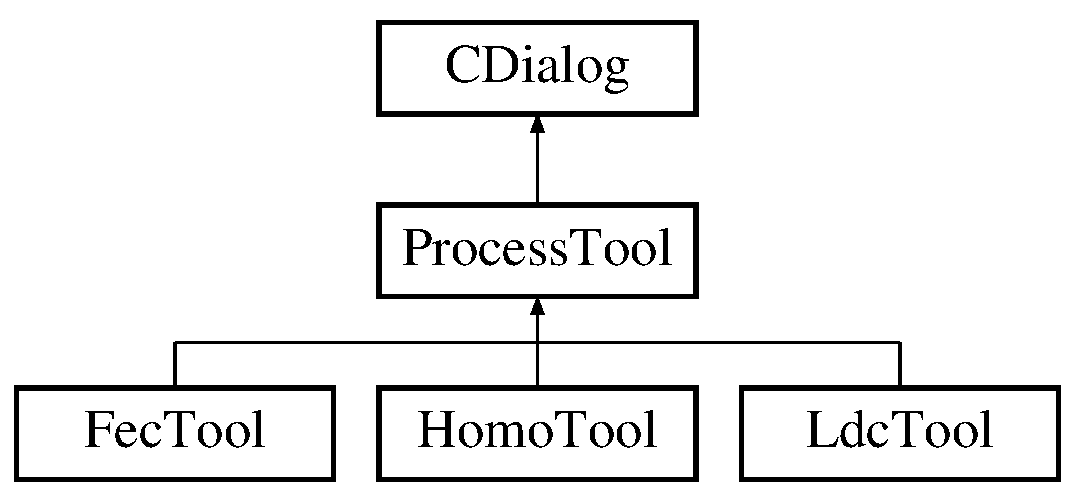
\includegraphics[height=3.000000cm]{class_process_tool}
\end{center}
\end{figure}
\subsection*{Public Types}
\begin{DoxyCompactItemize}
\item 
\mbox{\Hypertarget{class_process_tool_a476140737a8e6c273f9297bd384f8cae}\label{class_process_tool_a476140737a8e6c273f9297bd384f8cae}} 
enum \{ {\bfseries I\+DD} = 0
 \}
\end{DoxyCompactItemize}
\subsection*{Public Member Functions}
\begin{DoxyCompactItemize}
\item 
static \mbox{\hyperlink{class_process_tool}{Process\+Tool}} $\ast$ \mbox{\hyperlink{class_process_tool_a58b14d09ecf71dc46c978dc1afb56967}{Create\+Process\+Tool}} (C\+Wnd $\ast$p\+Owner, int n\+Type, Img\+File $\ast$p\+Image)
\item 
int \mbox{\hyperlink{class_process_tool_ab0e7d3a46484506a517325b938d537a0}{Get\+Process\+Tool\+ID}} ()
\item 
\mbox{\Hypertarget{class_process_tool_a52953e59d84e5e8178dbe7ed38fcec6c}\label{class_process_tool_a52953e59d84e5e8178dbe7ed38fcec6c}} 
{\bfseries Process\+Tool} (U\+I\+NT n\+I\+D\+Template, C\+Wnd $\ast$p\+Parent=N\+U\+LL)
\item 
virtual void \mbox{\hyperlink{class_process_tool_a50caa175198cece00b39a146715bf3eb}{Set\+Param}} (\mbox{\hyperlink{class_process_wrap}{Process\+Wrap}} $\ast$p\+Param)
\item 
virtual \mbox{\hyperlink{class_process_wrap}{Process\+Wrap}} $\ast$ \mbox{\hyperlink{class_process_tool_a355ebcf991f86f59f4241ea4345547fc}{Get\+Param}} ()
\item 
virtual void \mbox{\hyperlink{class_process_tool_a178bc06abf5a20220bd2306a14708a93}{Set\+Img\+File}} (Img\+File $\ast$p\+Image)
\item 
virtual Img\+File $\ast$ \mbox{\hyperlink{class_process_tool_abe1cbbab6613f24a752113a3ec4faaa8}{Get\+Img\+File}} ()
\item 
\mbox{\Hypertarget{class_process_tool_a644f45cdf995090c61975f6fa345333f}\label{class_process_tool_a644f45cdf995090c61975f6fa345333f}} 
afx\+\_\+msg void {\bfseries On\+Bn\+Clicked\+Cancel} ()
\item 
\mbox{\Hypertarget{class_process_tool_af707c18c69b52e97ea32b879c4fdc440}\label{class_process_tool_af707c18c69b52e97ea32b879c4fdc440}} 
afx\+\_\+msg void {\bfseries On\+Bn\+Clicked\+Ok} ()
\item 
\mbox{\Hypertarget{class_process_tool_a639a520f4af641c5253c6655c6b499c6}\label{class_process_tool_a639a520f4af641c5253c6655c6b499c6}} 
afx\+\_\+msg void {\bfseries On\+Update\+Toolbox} (C\+Cmd\+UI $\ast$p\+Cmd\+UI)
\item 
\mbox{\Hypertarget{class_process_tool_a1f856d66a4dd11a9ddd215a971866306}\label{class_process_tool_a1f856d66a4dd11a9ddd215a971866306}} 
afx\+\_\+msg void {\bfseries On\+Command\+Toolbox} (U\+I\+NT n\+Cmd)
\item 
\mbox{\Hypertarget{class_process_tool_a4aba1cb35feb212ea5771ad59e7e8427}\label{class_process_tool_a4aba1cb35feb212ea5771ad59e7e8427}} 
afx\+\_\+msg void {\bfseries On\+Destroy} ()
\end{DoxyCompactItemize}
\subsection*{Protected Member Functions}
\begin{DoxyCompactItemize}
\item 
\mbox{\Hypertarget{class_process_tool_a593e262bfa4f97671d404f17dc173a3a}\label{class_process_tool_a593e262bfa4f97671d404f17dc173a3a}} 
float {\bfseries Get\+Dlg\+Item\+Float} (int n\+ID)
\item 
\mbox{\Hypertarget{class_process_tool_acff1c8e2b44509bc0ab9ae4e51e61ddc}\label{class_process_tool_acff1c8e2b44509bc0ab9ae4e51e61ddc}} 
void {\bfseries Set\+Dlg\+Item\+Float} (int n\+ID, float f\+Value)
\item 
\mbox{\Hypertarget{class_process_tool_acf5cdf0b306dcf0a9bda434cb4098120}\label{class_process_tool_acf5cdf0b306dcf0a9bda434cb4098120}} 
virtual void {\bfseries Update\+Data} (B\+O\+OL b\+Save\+And\+Validate=T\+R\+UE)
\item 
\mbox{\Hypertarget{class_process_tool_ae1d455b1be56263db97e2cbb0e047d0a}\label{class_process_tool_ae1d455b1be56263db97e2cbb0e047d0a}} 
virtual void {\bfseries Post\+Nc\+Destroy} ()
\item 
void \mbox{\hyperlink{class_process_tool_aff87d429b43cdb20405a5036ec0a4d66}{On\+Save\+Parameter}} ()
\item 
void \mbox{\hyperlink{class_process_tool_a06656026e81c2da884f1130804aac780}{On\+Load\+Parameter}} ()
\end{DoxyCompactItemize}
\subsection*{Protected Attributes}
\begin{DoxyCompactItemize}
\item 
\mbox{\hyperlink{class_process_wrap}{Process\+Wrap}} $\ast$ \mbox{\hyperlink{class_process_tool_ae19c0d700f0a30bb0ca9d18e5397a562}{m\+\_\+p\+Process\+Wrap}}
\item 
\mbox{\hyperlink{class_process_view}{Process\+View}} $\ast$ \mbox{\hyperlink{class_process_tool_a775ff126073fabb52a8374c083058596}{m\+\_\+p\+Basic\+View}}
\end{DoxyCompactItemize}


\subsection{Detailed Description}
\mbox{\hyperlink{class_process_tool}{Process\+Tool}} is the abstract class which is used to control the settings of a process with UI in a dialog box. A \mbox{\hyperlink{class_process_tool}{Process\+Tool}} class consistent of a \mbox{\hyperlink{class_process_view}{Process\+View}} member to display the processed image and a \mbox{\hyperlink{class_process_wrap}{Process\+Wrap}} class member to aintain the process related parameters and L\+UT data. \mbox{\hyperlink{class_process_tool}{Process\+Tool}} is the bridge class between \mbox{\hyperlink{class_work_view}{Work\+View}} and the Process. The application use \mbox{\hyperlink{class_process_tool}{Process\+Tool}} to access the specified process stuff. 

\subsection{Member Function Documentation}
\mbox{\Hypertarget{class_process_tool_a58b14d09ecf71dc46c978dc1afb56967}\label{class_process_tool_a58b14d09ecf71dc46c978dc1afb56967}} 
\index{Process\+Tool@{Process\+Tool}!Create\+Process\+Tool@{Create\+Process\+Tool}}
\index{Create\+Process\+Tool@{Create\+Process\+Tool}!Process\+Tool@{Process\+Tool}}
\subsubsection{\texorpdfstring{Create\+Process\+Tool()}{CreateProcessTool()}}
{\footnotesize\ttfamily \mbox{\hyperlink{class_process_tool}{Process\+Tool}} $\ast$ Process\+Tool\+::\+Create\+Process\+Tool (\begin{DoxyParamCaption}\item[{C\+Wnd $\ast$}]{p\+Owner,  }\item[{int}]{n\+Type,  }\item[{Img\+File $\ast$}]{p\+Image }\end{DoxyParamCaption})}

Create the derrived class of the specified process typr


\begin{DoxyParams}{Parameters}
{\em p\+Owner} & parent window of the \mbox{\hyperlink{class_process_tool}{Process\+Tool}}, the \mbox{\hyperlink{class_work_view}{Work\+View}} class \\
\hline
{\em n\+Type} & type of \mbox{\hyperlink{class_process_tool}{Process\+Tool}} n\+Type = I\+D\+D\+\_\+\+F\+EC F\+EC process tool n\+Type = I\+D\+D\+\_\+\+L\+DC L\+DC process tool \\
\hline
{\em p\+Image} & the original image to be processed from \\
\hline
\end{DoxyParams}
\begin{DoxyReturn}{Returns}
the derrived \mbox{\hyperlink{class_process_tool}{Process\+Tool}} class pointer of the specified process. 
\end{DoxyReturn}
\mbox{\Hypertarget{class_process_tool_abe1cbbab6613f24a752113a3ec4faaa8}\label{class_process_tool_abe1cbbab6613f24a752113a3ec4faaa8}} 
\index{Process\+Tool@{Process\+Tool}!Get\+Img\+File@{Get\+Img\+File}}
\index{Get\+Img\+File@{Get\+Img\+File}!Process\+Tool@{Process\+Tool}}
\subsubsection{\texorpdfstring{Get\+Img\+File()}{GetImgFile()}}
{\footnotesize\ttfamily Img\+File $\ast$ Process\+Tool\+::\+Get\+Img\+File (\begin{DoxyParamCaption}{ }\end{DoxyParamCaption})\hspace{0.3cm}{\ttfamily [virtual]}}

Gets the processed image in \mbox{\hyperlink{class_process_view}{Process\+View}} of this \mbox{\hyperlink{class_process_tool}{Process\+Tool}}. \mbox{\Hypertarget{class_process_tool_a355ebcf991f86f59f4241ea4345547fc}\label{class_process_tool_a355ebcf991f86f59f4241ea4345547fc}} 
\index{Process\+Tool@{Process\+Tool}!Get\+Param@{Get\+Param}}
\index{Get\+Param@{Get\+Param}!Process\+Tool@{Process\+Tool}}
\subsubsection{\texorpdfstring{Get\+Param()}{GetParam()}}
{\footnotesize\ttfamily virtual \mbox{\hyperlink{class_process_wrap}{Process\+Wrap}}$\ast$ Get\+Param (\begin{DoxyParamCaption}{ }\end{DoxyParamCaption})\hspace{0.3cm}{\ttfamily [inline]}, {\ttfamily [virtual]}}

Gets the \mbox{\hyperlink{class_process_wrap}{Process\+Wrap}} class pointer of the process tool. 

Reimplemented in \mbox{\hyperlink{class_ldc_tool_af9828a2daf501b328a07dd8fa3d6abeb}{Ldc\+Tool}}, \mbox{\hyperlink{class_fec_tool_acccda5a312354ec0dcd215de8ed7ac03}{Fec\+Tool}}, and \mbox{\hyperlink{class_homo_tool_a497eb4f1812d3f38ea6657c35d64bf31}{Homo\+Tool}}.

\mbox{\Hypertarget{class_process_tool_ab0e7d3a46484506a517325b938d537a0}\label{class_process_tool_ab0e7d3a46484506a517325b938d537a0}} 
\index{Process\+Tool@{Process\+Tool}!Get\+Process\+Tool\+ID@{Get\+Process\+Tool\+ID}}
\index{Get\+Process\+Tool\+ID@{Get\+Process\+Tool\+ID}!Process\+Tool@{Process\+Tool}}
\subsubsection{\texorpdfstring{Get\+Process\+Tool\+I\+D()}{GetProcessToolID()}}
{\footnotesize\ttfamily int Get\+Process\+Tool\+ID (\begin{DoxyParamCaption}{ }\end{DoxyParamCaption})\hspace{0.3cm}{\ttfamily [inline]}}

Gets the \mbox{\hyperlink{class_process_tool}{Process\+Tool}} ID. \mbox{\Hypertarget{class_process_tool_a06656026e81c2da884f1130804aac780}\label{class_process_tool_a06656026e81c2da884f1130804aac780}} 
\index{Process\+Tool@{Process\+Tool}!On\+Load\+Parameter@{On\+Load\+Parameter}}
\index{On\+Load\+Parameter@{On\+Load\+Parameter}!Process\+Tool@{Process\+Tool}}
\subsubsection{\texorpdfstring{On\+Load\+Parameter()}{OnLoadParameter()}}
{\footnotesize\ttfamily void Process\+Tool\+::\+On\+Load\+Parameter (\begin{DoxyParamCaption}{ }\end{DoxyParamCaption})\hspace{0.3cm}{\ttfamily [protected]}}

UI request to load process parameters \mbox{\Hypertarget{class_process_tool_aff87d429b43cdb20405a5036ec0a4d66}\label{class_process_tool_aff87d429b43cdb20405a5036ec0a4d66}} 
\index{Process\+Tool@{Process\+Tool}!On\+Save\+Parameter@{On\+Save\+Parameter}}
\index{On\+Save\+Parameter@{On\+Save\+Parameter}!Process\+Tool@{Process\+Tool}}
\subsubsection{\texorpdfstring{On\+Save\+Parameter()}{OnSaveParameter()}}
{\footnotesize\ttfamily void Process\+Tool\+::\+On\+Save\+Parameter (\begin{DoxyParamCaption}{ }\end{DoxyParamCaption})\hspace{0.3cm}{\ttfamily [protected]}}

UI request to save process parameters \mbox{\Hypertarget{class_process_tool_a178bc06abf5a20220bd2306a14708a93}\label{class_process_tool_a178bc06abf5a20220bd2306a14708a93}} 
\index{Process\+Tool@{Process\+Tool}!Set\+Img\+File@{Set\+Img\+File}}
\index{Set\+Img\+File@{Set\+Img\+File}!Process\+Tool@{Process\+Tool}}
\subsubsection{\texorpdfstring{Set\+Img\+File()}{SetImgFile()}}
{\footnotesize\ttfamily void Process\+Tool\+::\+Set\+Img\+File (\begin{DoxyParamCaption}\item[{Img\+File $\ast$}]{p\+Image }\end{DoxyParamCaption})\hspace{0.3cm}{\ttfamily [virtual]}}

Sets the image to be processed from. The processed imaged won\textquotesingle{}t replace this original image. 

Reimplemented in \mbox{\hyperlink{class_ldc_tool_a07d1a547f02d4dea6a480c1be875a685}{Ldc\+Tool}}, \mbox{\hyperlink{class_fec_tool_ac99805fa120b8bb7a21fc08382a875c1}{Fec\+Tool}}, and \mbox{\hyperlink{class_homo_tool_af43fe8ae0732dffbeb35b59058509af2}{Homo\+Tool}}.

\mbox{\Hypertarget{class_process_tool_a50caa175198cece00b39a146715bf3eb}\label{class_process_tool_a50caa175198cece00b39a146715bf3eb}} 
\index{Process\+Tool@{Process\+Tool}!Set\+Param@{Set\+Param}}
\index{Set\+Param@{Set\+Param}!Process\+Tool@{Process\+Tool}}
\subsubsection{\texorpdfstring{Set\+Param()}{SetParam()}}
{\footnotesize\ttfamily virtual void Set\+Param (\begin{DoxyParamCaption}\item[{\mbox{\hyperlink{class_process_wrap}{Process\+Wrap}} $\ast$}]{p\+Param }\end{DoxyParamCaption})\hspace{0.3cm}{\ttfamily [inline]}, {\ttfamily [virtual]}}

Copys contents of process parameters into related \mbox{\hyperlink{class_process_wrap}{Process\+Wrap}}. 

Reimplemented in \mbox{\hyperlink{class_ldc_tool_a1c98303e0ab2dfea1f1dcca8f1548307}{Ldc\+Tool}}, \mbox{\hyperlink{class_fec_tool_acd6cd4230cb79fe0cb1053c588f91806}{Fec\+Tool}}, and \mbox{\hyperlink{class_homo_tool_a69965855ba23da88abe7903ad58c20c6}{Homo\+Tool}}.



\subsection{Member Data Documentation}
\mbox{\Hypertarget{class_process_tool_a775ff126073fabb52a8374c083058596}\label{class_process_tool_a775ff126073fabb52a8374c083058596}} 
\index{Process\+Tool@{Process\+Tool}!m\+\_\+p\+Basic\+View@{m\+\_\+p\+Basic\+View}}
\index{m\+\_\+p\+Basic\+View@{m\+\_\+p\+Basic\+View}!Process\+Tool@{Process\+Tool}}
\subsubsection{\texorpdfstring{m\+\_\+p\+Basic\+View}{m\_pBasicView}}
{\footnotesize\ttfamily \mbox{\hyperlink{class_process_view}{Process\+View}}$\ast$ Process\+Tool\+::m\+\_\+p\+Basic\+View\hspace{0.3cm}{\ttfamily [protected]}}

pointer to processed image viewer \mbox{\Hypertarget{class_process_tool_ae19c0d700f0a30bb0ca9d18e5397a562}\label{class_process_tool_ae19c0d700f0a30bb0ca9d18e5397a562}} 
\index{Process\+Tool@{Process\+Tool}!m\+\_\+p\+Process\+Wrap@{m\+\_\+p\+Process\+Wrap}}
\index{m\+\_\+p\+Process\+Wrap@{m\+\_\+p\+Process\+Wrap}!Process\+Tool@{Process\+Tool}}
\subsubsection{\texorpdfstring{m\+\_\+p\+Process\+Wrap}{m\_pProcessWrap}}
{\footnotesize\ttfamily \mbox{\hyperlink{class_process_wrap}{Process\+Wrap}}$\ast$ Process\+Tool\+::m\+\_\+p\+Process\+Wrap\hspace{0.3cm}{\ttfamily [protected]}}

pointer to parameter capsulator class 

The documentation for this class was generated from the following files\+:\begin{DoxyCompactItemize}
\item 
i\+Optics/\mbox{\hyperlink{_process_tool_8h}{Process\+Tool.\+h}}\item 
i\+Optics/Process\+Tool.\+cpp\end{DoxyCompactItemize}

\hypertarget{class_process_view}{}\section{Process\+View Class Reference}
\label{class_process_view}\index{Process\+View@{Process\+View}}


\mbox{\hyperlink{class_process_view}{Process\+View}} is the basic image viewer for processing image viewing. It handles the video rendering process by the specified process. It is controlled by its process correspondent \mbox{\hyperlink{class_process_tool}{Process\+Tool}}. It also can display gride lines on the image window.  




{\ttfamily \#include $<$Process\+View.\+h$>$}

Inheritance diagram for Process\+View\+:\begin{figure}[H]
\begin{center}
\leavevmode
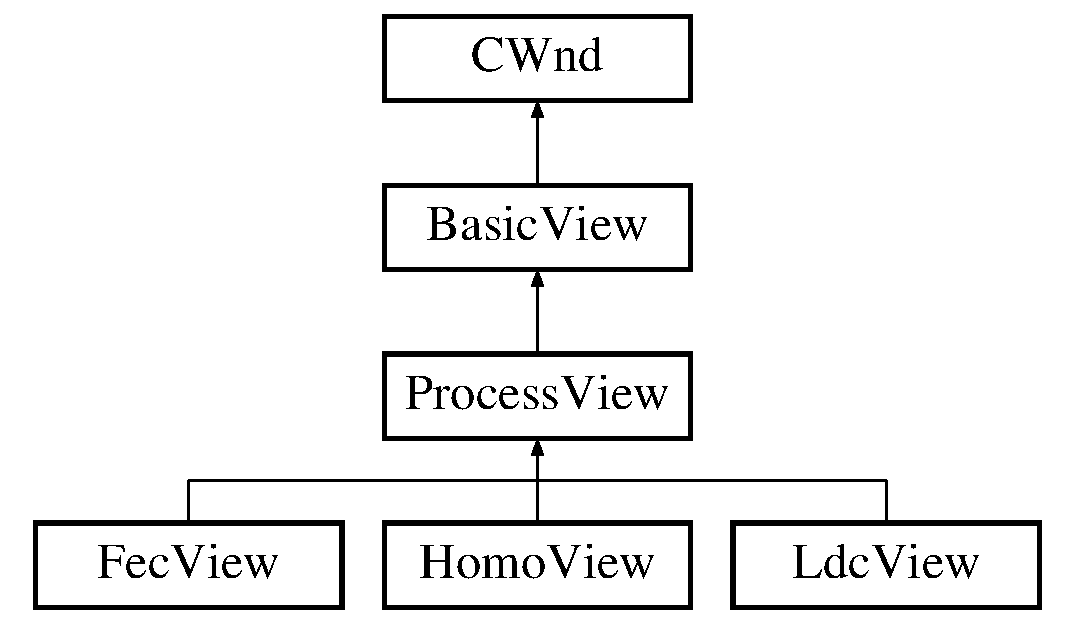
\includegraphics[height=4.000000cm]{class_process_view}
\end{center}
\end{figure}
\subsection*{Public Member Functions}
\begin{DoxyCompactItemize}
\item 
\mbox{\Hypertarget{class_process_view_a5b907e6d6920c9540fb6cefb287f5570}\label{class_process_view_a5b907e6d6920c9540fb6cefb287f5570}} 
virtual void {\bfseries Set\+Img\+File} (Img\+File $\ast$p\+Img)
\item 
\mbox{\Hypertarget{class_process_view_a464aa6e662a5fe7670bf352f496ba60c}\label{class_process_view_a464aa6e662a5fe7670bf352f496ba60c}} 
virtual void {\bfseries Set\+Param} (\mbox{\hyperlink{class_process_wrap}{Process\+Wrap}} $\ast$p\+Wrapper)
\item 
\mbox{\Hypertarget{class_process_view_ae0f8b6cc39a64ece62ef206014cbc18e}\label{class_process_view_ae0f8b6cc39a64ece62ef206014cbc18e}} 
B\+O\+OL {\bfseries Set\+Scroll\+Pos} (int nX, int nY)
\item 
\mbox{\Hypertarget{class_process_view_a4877a8e9b9a0d1afd9553e3c71142196}\label{class_process_view_a4877a8e9b9a0d1afd9553e3c71142196}} 
virtual void {\bfseries Post\+Nc\+Destroy} ()
\item 
\mbox{\Hypertarget{class_process_view_a05940c5be5b5b213ff04c0088be1a865}\label{class_process_view_a05940c5be5b5b213ff04c0088be1a865}} 
afx\+\_\+msg int {\bfseries On\+Create} (L\+P\+C\+R\+E\+A\+T\+E\+S\+T\+R\+U\+CT lp\+Create\+Struct)
\item 
\mbox{\Hypertarget{class_process_view_ada60d6fb93c2746f70c4074feb9279b5}\label{class_process_view_ada60d6fb93c2746f70c4074feb9279b5}} 
afx\+\_\+msg void {\bfseries On\+Paint} ()
\item 
\mbox{\Hypertarget{class_process_view_a09f448c77e2887a5747e3036bc739f7a}\label{class_process_view_a09f448c77e2887a5747e3036bc739f7a}} 
afx\+\_\+msg void {\bfseries On\+Preview} ()
\item 
\mbox{\Hypertarget{class_process_view_a0538625c6a1599287375668ef83dfd55}\label{class_process_view_a0538625c6a1599287375668ef83dfd55}} 
afx\+\_\+msg void {\bfseries On\+Size} (U\+I\+NT n\+Type, int cx, int cy)
\item 
\mbox{\Hypertarget{class_process_view_a60b5b22454247990d2002555230dceb7}\label{class_process_view_a60b5b22454247990d2002555230dceb7}} 
afx\+\_\+msg void {\bfseries On\+H\+Scroll} (U\+I\+NT n\+S\+B\+Code, U\+I\+NT n\+Pos, C\+Scroll\+Bar $\ast$p\+Scroll\+Bar)
\item 
\mbox{\Hypertarget{class_process_view_a6cd442b45537d007e354f6d6bb59a778}\label{class_process_view_a6cd442b45537d007e354f6d6bb59a778}} 
afx\+\_\+msg void {\bfseries On\+V\+Scroll} (U\+I\+NT n\+S\+B\+Code, U\+I\+NT n\+Pos, C\+Scroll\+Bar $\ast$p\+Scroll\+Bar)
\item 
\mbox{\Hypertarget{class_process_view_a83b03b4d575bcb06ebf6bdd470c01942}\label{class_process_view_a83b03b4d575bcb06ebf6bdd470c01942}} 
afx\+\_\+msg void {\bfseries On\+View\+Gride} ()
\item 
\mbox{\Hypertarget{class_process_view_acbb45aa45b32a59abd0b9a2193d7183e}\label{class_process_view_acbb45aa45b32a59abd0b9a2193d7183e}} 
afx\+\_\+msg void {\bfseries On\+Update\+View\+Gride} (C\+Cmd\+UI $\ast$p\+Cmd\+UI)
\item 
\mbox{\Hypertarget{class_process_view_a543224f665b9e4a819e753851815fc3d}\label{class_process_view_a543224f665b9e4a819e753851815fc3d}} 
afx\+\_\+msg void {\bfseries On\+Update\+Toolbox} (C\+Cmd\+UI $\ast$p\+Cmd\+UI)
\item 
\mbox{\Hypertarget{class_process_view_aceb4f73ef0470ac2defa7240234ff8b2}\label{class_process_view_aceb4f73ef0470ac2defa7240234ff8b2}} 
afx\+\_\+msg void {\bfseries On\+Command\+Toolbox} (U\+I\+NT n\+Cmd)
\item 
\mbox{\Hypertarget{class_process_view_a20ed42b9ec53e1c8a06c4583569c71fc}\label{class_process_view_a20ed42b9ec53e1c8a06c4583569c71fc}} 
afx\+\_\+msg void {\bfseries On\+View\+Zoomin} ()
\item 
\mbox{\Hypertarget{class_process_view_a20aa12d6a33b71fc6a303c8a1af95268}\label{class_process_view_a20aa12d6a33b71fc6a303c8a1af95268}} 
afx\+\_\+msg void {\bfseries On\+View\+Zoomout} ()
\end{DoxyCompactItemize}
\subsection*{Public Attributes}
\begin{DoxyCompactItemize}
\item 
\mbox{\Hypertarget{class_process_view_aeef37b8953cb3c432954240c91e98a5d}\label{class_process_view_aeef37b8953cb3c432954240c91e98a5d}} 
B\+O\+OL {\bfseries m\+\_\+b\+Show\+Gride}
\item 
\mbox{\Hypertarget{class_process_view_a7c7fc0bd7d0416172e7d00cf682f2bb5}\label{class_process_view_a7c7fc0bd7d0416172e7d00cf682f2bb5}} 
\mbox{\hyperlink{class_gride}{Gride}} {\bfseries m\+\_\+gride}
\item 
\mbox{\Hypertarget{class_process_view_adc0115d468bba213de87ed1513fc673f}\label{class_process_view_adc0115d468bba213de87ed1513fc673f}} 
Img\+File $\ast$ {\bfseries m\+\_\+p\+Original\+Img}
\end{DoxyCompactItemize}
\subsection*{Protected Member Functions}
\begin{DoxyCompactItemize}
\item 
\mbox{\Hypertarget{class_process_view_af3bae21acece6d1027a873abb06bc26f}\label{class_process_view_af3bae21acece6d1027a873abb06bc26f}} 
virtual B\+O\+OL {\bfseries Pos\+Map} (int u, int v, float \&x, float \&y)
\item 
\mbox{\Hypertarget{class_process_view_ae4c2be79e8aa2b37e2761801555975ae}\label{class_process_view_ae4c2be79e8aa2b37e2761801555975ae}} 
virtual C\+O\+L\+O\+R\+R\+EF {\bfseries Get\+Color} (B\+Y\+TE $\ast$p\+Src, int stride, float x, float y)
\end{DoxyCompactItemize}
\subsection*{Additional Inherited Members}


\subsection{Detailed Description}
\mbox{\hyperlink{class_process_view}{Process\+View}} is the basic image viewer for processing image viewing. It handles the video rendering process by the specified process. It is controlled by its process correspondent \mbox{\hyperlink{class_process_tool}{Process\+Tool}}. It also can display gride lines on the image window. 

\begin{DoxySeeAlso}{See also}
\mbox{\hyperlink{class_process_tool}{Process\+Tool}}. 
\end{DoxySeeAlso}


The documentation for this class was generated from the following files\+:\begin{DoxyCompactItemize}
\item 
i\+Optics/Process\+View.\+h\item 
i\+Optics/Process\+View.\+cpp\end{DoxyCompactItemize}

\hypertarget{class_process_wrap}{}\section{Process\+Wrap Class Reference}
\label{class_process_wrap}\index{Process\+Wrap@{Process\+Wrap}}


wrap process parameters  




{\ttfamily \#include $<$Process\+Tool.\+h$>$}

Inheritance diagram for Process\+Wrap\+:\begin{figure}[H]
\begin{center}
\leavevmode
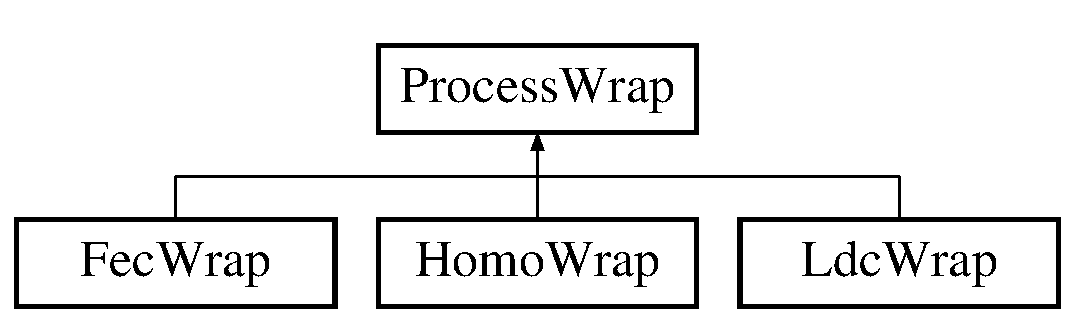
\includegraphics[height=2.000000cm]{class_process_wrap}
\end{center}
\end{figure}
\subsection*{Public Member Functions}
\begin{DoxyCompactItemize}
\item 
virtual void \mbox{\hyperlink{class_process_wrap_a6c7130837d4713b0462f42cfc25aca98}{Set\+Param}} (void $\ast$p\+Param)
\item 
virtual void \mbox{\hyperlink{class_process_wrap_a22910a91f52147b8631b7e880509996e}{Make\+Map\+Table}} ()=0
\item 
virtual B\+O\+OL \mbox{\hyperlink{class_process_wrap_a536c940a16b6331109aa5d30763974fe}{Pos\+Map}} (int u, int v, float \&x, float \&y)=0
\item 
\mbox{\hyperlink{struct___point_double}{Point\+Double}} $\ast$ \mbox{\hyperlink{class_process_wrap_a69ce0c8809b27258dd416b4a806b347d}{Get\+Lut\+Table}} ()
\item 
int \mbox{\hyperlink{class_process_wrap_a14eafff7a715fb84f7b3a3b2dc37bd0c}{Lut\+Columns}} ()
\item 
int \mbox{\hyperlink{class_process_wrap_a805d35317ea071adec5d6a4497608e43}{Lut\+Rows}} ()
\item 
void \mbox{\hyperlink{class_process_wrap_a8a33b5609c68b5273cddbdd28dd9881b}{Reset\+Lut\+Data}} ()
\item 
double \mbox{\hyperlink{class_process_wrap_a21c63fcb4fec0ca44ad0d8dcd41d1fa3}{Get\+Lut\+DataX}} (int x, int y)
\item 
double \mbox{\hyperlink{class_process_wrap_a644d6814dc0d8d744470d81862900ff8}{Get\+Lut\+DataY}} (int x, int y)
\item 
void \mbox{\hyperlink{class_process_wrap_a8e4e346bc28b54e1f789ed6c7d3cd0f4}{Set\+Lut\+DataX}} (int x, int y, double value)
\item 
void \mbox{\hyperlink{class_process_wrap_a86c91328a42d3a3bee76507595050fd1}{Set\+Lut\+DataY}} (int x, int y, double value)
\item 
virtual B\+O\+OL \mbox{\hyperlink{class_process_wrap_aa5d4361a42a7a65cac877beb6d4ffa97}{Save\+Parameter}} (L\+P\+C\+T\+S\+TR filename)=0
\item 
virtual B\+O\+OL \mbox{\hyperlink{class_process_wrap_a1cb75a423ff8f5ef736fc00a34792493}{Load\+Parameter}} (L\+P\+C\+T\+S\+TR filename)=0
\end{DoxyCompactItemize}
\subsection*{Protected Attributes}
\begin{DoxyCompactItemize}
\item 
int \mbox{\hyperlink{class_process_wrap_aa7b1b1ab80a42889823b0357de5d3c4a}{cx\+Lut}}
\item 
int \mbox{\hyperlink{class_process_wrap_ab18b53afcd7d7b0d941a45a9c89e177c}{cy\+Lut}}
\item 
\mbox{\hyperlink{struct___point_double}{Point\+Double}} $\ast$ \mbox{\hyperlink{class_process_wrap_a39358a35e911d631f6bd46f6bf815d25}{lut}}
\end{DoxyCompactItemize}


\subsection{Detailed Description}
wrap process parameters 

The data of process parameters are depedent on individual process tool. Each tool will produce L\+UT data, which is maintained by this class. The \mbox{\hyperlink{class_process_wrap}{Process\+Wrap}} keeps process\textquotesingle{}s parameters and allocate memory space for L\+UT. The struct of a Process\textquotesingle{}s parameter is defined by each Process and decalred in \mbox{\hyperlink{common_8h}{common.\+h}} \begin{DoxySeeAlso}{See also}
\mbox{\hyperlink{class_process_view}{Process\+View}} \mbox{\hyperlink{class_process_wrap}{Process\+Wrap}} 
\end{DoxySeeAlso}


\subsection{Member Function Documentation}
\mbox{\Hypertarget{class_process_wrap_a21c63fcb4fec0ca44ad0d8dcd41d1fa3}\label{class_process_wrap_a21c63fcb4fec0ca44ad0d8dcd41d1fa3}} 
\index{Process\+Wrap@{Process\+Wrap}!Get\+Lut\+DataX@{Get\+Lut\+DataX}}
\index{Get\+Lut\+DataX@{Get\+Lut\+DataX}!Process\+Wrap@{Process\+Wrap}}
\subsubsection{\texorpdfstring{Get\+Lut\+Data\+X()}{GetLutDataX()}}
{\footnotesize\ttfamily double Process\+Wrap\+::\+Get\+Lut\+DataX (\begin{DoxyParamCaption}\item[{int}]{x,  }\item[{int}]{y }\end{DoxyParamCaption})\hspace{0.3cm}{\ttfamily [inline]}}

Get normalized X coordinate the L\+UT in the position (X,Y) which is on processed image \mbox{\Hypertarget{class_process_wrap_a644d6814dc0d8d744470d81862900ff8}\label{class_process_wrap_a644d6814dc0d8d744470d81862900ff8}} 
\index{Process\+Wrap@{Process\+Wrap}!Get\+Lut\+DataY@{Get\+Lut\+DataY}}
\index{Get\+Lut\+DataY@{Get\+Lut\+DataY}!Process\+Wrap@{Process\+Wrap}}
\subsubsection{\texorpdfstring{Get\+Lut\+Data\+Y()}{GetLutDataY()}}
{\footnotesize\ttfamily double Process\+Wrap\+::\+Get\+Lut\+DataY (\begin{DoxyParamCaption}\item[{int}]{x,  }\item[{int}]{y }\end{DoxyParamCaption})\hspace{0.3cm}{\ttfamily [inline]}}

Get normalized Y coordinate the L\+UT in the position (X,Y) which is on processed image \mbox{\Hypertarget{class_process_wrap_a69ce0c8809b27258dd416b4a806b347d}\label{class_process_wrap_a69ce0c8809b27258dd416b4a806b347d}} 
\index{Process\+Wrap@{Process\+Wrap}!Get\+Lut\+Table@{Get\+Lut\+Table}}
\index{Get\+Lut\+Table@{Get\+Lut\+Table}!Process\+Wrap@{Process\+Wrap}}
\subsubsection{\texorpdfstring{Get\+Lut\+Table()}{GetLutTable()}}
{\footnotesize\ttfamily \mbox{\hyperlink{struct___point_double}{Point\+Double}}$\ast$ Get\+Lut\+Table (\begin{DoxyParamCaption}{ }\end{DoxyParamCaption})\hspace{0.3cm}{\ttfamily [inline]}}

Gets the start address of L\+UT buffer \mbox{\Hypertarget{class_process_wrap_a1cb75a423ff8f5ef736fc00a34792493}\label{class_process_wrap_a1cb75a423ff8f5ef736fc00a34792493}} 
\index{Process\+Wrap@{Process\+Wrap}!Load\+Parameter@{Load\+Parameter}}
\index{Load\+Parameter@{Load\+Parameter}!Process\+Wrap@{Process\+Wrap}}
\subsubsection{\texorpdfstring{Load\+Parameter()}{LoadParameter()}}
{\footnotesize\ttfamily virtual B\+O\+OL Load\+Parameter (\begin{DoxyParamCaption}\item[{L\+P\+C\+T\+S\+TR}]{filename }\end{DoxyParamCaption})\hspace{0.3cm}{\ttfamily [pure virtual]}}

Read process specified parameters from a file. The format of data can be defined dependently by the correspondent \mbox{\hyperlink{class_process_wrap}{Process\+Wrap}} class. 

Implemented in \mbox{\hyperlink{class_ldc_wrap_a5409cdfe65bc28ec3779f35eb3af22b4}{Ldc\+Wrap}}, \mbox{\hyperlink{class_fec_wrap_a3f55d86b6b99108b360b66d1d180a66c}{Fec\+Wrap}}, and \mbox{\hyperlink{class_homo_wrap_a5409cdfe65bc28ec3779f35eb3af22b4}{Homo\+Wrap}}.

\mbox{\Hypertarget{class_process_wrap_a14eafff7a715fb84f7b3a3b2dc37bd0c}\label{class_process_wrap_a14eafff7a715fb84f7b3a3b2dc37bd0c}} 
\index{Process\+Wrap@{Process\+Wrap}!Lut\+Columns@{Lut\+Columns}}
\index{Lut\+Columns@{Lut\+Columns}!Process\+Wrap@{Process\+Wrap}}
\subsubsection{\texorpdfstring{Lut\+Columns()}{LutColumns()}}
{\footnotesize\ttfamily int Lut\+Columns (\begin{DoxyParamCaption}{ }\end{DoxyParamCaption})\hspace{0.3cm}{\ttfamily [inline]}}

Gets the numbers of column of the L\+UT, including bondary \mbox{\Hypertarget{class_process_wrap_a805d35317ea071adec5d6a4497608e43}\label{class_process_wrap_a805d35317ea071adec5d6a4497608e43}} 
\index{Process\+Wrap@{Process\+Wrap}!Lut\+Rows@{Lut\+Rows}}
\index{Lut\+Rows@{Lut\+Rows}!Process\+Wrap@{Process\+Wrap}}
\subsubsection{\texorpdfstring{Lut\+Rows()}{LutRows()}}
{\footnotesize\ttfamily int Lut\+Rows (\begin{DoxyParamCaption}{ }\end{DoxyParamCaption})\hspace{0.3cm}{\ttfamily [inline]}}

Gets the numbers of rows of the L\+UT, including bondary \mbox{\Hypertarget{class_process_wrap_a22910a91f52147b8631b7e880509996e}\label{class_process_wrap_a22910a91f52147b8631b7e880509996e}} 
\index{Process\+Wrap@{Process\+Wrap}!Make\+Map\+Table@{Make\+Map\+Table}}
\index{Make\+Map\+Table@{Make\+Map\+Table}!Process\+Wrap@{Process\+Wrap}}
\subsubsection{\texorpdfstring{Make\+Map\+Table()}{MakeMapTable()}}
{\footnotesize\ttfamily virtual void Process\+Wrap\+::\+Make\+Map\+Table (\begin{DoxyParamCaption}{ }\end{DoxyParamCaption})\hspace{0.3cm}{\ttfamily [pure virtual]}}

Create the L\+UT data according its processing parameters 

Implemented in \mbox{\hyperlink{class_fec_wrap_ac1c213fd03716ce0bb6430e2d2bf7962}{Fec\+Wrap}}, \mbox{\hyperlink{class_ldc_wrap_a0c6a77b5857bf0bc57c935b8612df9ad}{Ldc\+Wrap}}, and \mbox{\hyperlink{class_homo_wrap_a04c5506434d9afe322bfd6c08c51868f}{Homo\+Wrap}}.

\mbox{\Hypertarget{class_process_wrap_a536c940a16b6331109aa5d30763974fe}\label{class_process_wrap_a536c940a16b6331109aa5d30763974fe}} 
\index{Process\+Wrap@{Process\+Wrap}!Pos\+Map@{Pos\+Map}}
\index{Pos\+Map@{Pos\+Map}!Process\+Wrap@{Process\+Wrap}}
\subsubsection{\texorpdfstring{Pos\+Map()}{PosMap()}}
{\footnotesize\ttfamily virtual B\+O\+OL Process\+Wrap\+::\+Pos\+Map (\begin{DoxyParamCaption}\item[{int}]{u,  }\item[{int}]{v,  }\item[{float \&}]{x,  }\item[{float \&}]{y }\end{DoxyParamCaption})\hspace{0.3cm}{\ttfamily [pure virtual]}}

Position mapping from processed image to ideal position of original image 
\begin{DoxyParams}[1]{Parameters}
\mbox{\tt in}  & {\em u} & \mbox{[}0$\sim$sz\+Output.cx) in rocessed image \\
\hline
\mbox{\tt in}  & {\em v} & \mbox{[}0$\sim$sz\+Output.cy) in rocessed image \\
\hline
\mbox{\tt out}  & {\em x} & \mbox{[}0$\sim$sz\+Input.cx) in rocessed image \\
\hline
\mbox{\tt out}  & {\em y} & \mbox{[}0$\sim$sz\+Input.cy) in rocessed image \\
\hline
\end{DoxyParams}


Implemented in \mbox{\hyperlink{class_fec_wrap_a50575c4f361b71e6de2e8c1073b4a26a}{Fec\+Wrap}}, \mbox{\hyperlink{class_ldc_wrap_ad427e8c69a36be35bf5b95afa1d4fca3}{Ldc\+Wrap}}, and \mbox{\hyperlink{class_homo_wrap_a028ad1fea13805568dbe891f51dec7b2}{Homo\+Wrap}}.

\mbox{\Hypertarget{class_process_wrap_a8a33b5609c68b5273cddbdd28dd9881b}\label{class_process_wrap_a8a33b5609c68b5273cddbdd28dd9881b}} 
\index{Process\+Wrap@{Process\+Wrap}!Reset\+Lut\+Data@{Reset\+Lut\+Data}}
\index{Reset\+Lut\+Data@{Reset\+Lut\+Data}!Process\+Wrap@{Process\+Wrap}}
\subsubsection{\texorpdfstring{Reset\+Lut\+Data()}{ResetLutData()}}
{\footnotesize\ttfamily void Reset\+Lut\+Data (\begin{DoxyParamCaption}{ }\end{DoxyParamCaption})\hspace{0.3cm}{\ttfamily [inline]}}

Cleans the L\+UT buffer \mbox{\Hypertarget{class_process_wrap_aa5d4361a42a7a65cac877beb6d4ffa97}\label{class_process_wrap_aa5d4361a42a7a65cac877beb6d4ffa97}} 
\index{Process\+Wrap@{Process\+Wrap}!Save\+Parameter@{Save\+Parameter}}
\index{Save\+Parameter@{Save\+Parameter}!Process\+Wrap@{Process\+Wrap}}
\subsubsection{\texorpdfstring{Save\+Parameter()}{SaveParameter()}}
{\footnotesize\ttfamily virtual B\+O\+OL Save\+Parameter (\begin{DoxyParamCaption}\item[{L\+P\+C\+T\+S\+TR}]{filename }\end{DoxyParamCaption})\hspace{0.3cm}{\ttfamily [pure virtual]}}

Save process specified parameters in a file. The format of data can be defined dependently in this function. 

Implemented in \mbox{\hyperlink{class_fec_wrap_abd377e205b42ec6725293c3c9ff76a34}{Fec\+Wrap}}, \mbox{\hyperlink{class_ldc_wrap_aafd5595ef17a6be3074186204c39a550}{Ldc\+Wrap}}, and \mbox{\hyperlink{class_homo_wrap_aafd5595ef17a6be3074186204c39a550}{Homo\+Wrap}}.

\mbox{\Hypertarget{class_process_wrap_a8e4e346bc28b54e1f789ed6c7d3cd0f4}\label{class_process_wrap_a8e4e346bc28b54e1f789ed6c7d3cd0f4}} 
\index{Process\+Wrap@{Process\+Wrap}!Set\+Lut\+DataX@{Set\+Lut\+DataX}}
\index{Set\+Lut\+DataX@{Set\+Lut\+DataX}!Process\+Wrap@{Process\+Wrap}}
\subsubsection{\texorpdfstring{Set\+Lut\+Data\+X()}{SetLutDataX()}}
{\footnotesize\ttfamily void Process\+Wrap\+::\+Set\+Lut\+DataX (\begin{DoxyParamCaption}\item[{int}]{x,  }\item[{int}]{y,  }\item[{double}]{value }\end{DoxyParamCaption})\hspace{0.3cm}{\ttfamily [inline]}}

Set normalized X coordinate the L\+UT in the position (X,Y) which is on processed image \mbox{\Hypertarget{class_process_wrap_a86c91328a42d3a3bee76507595050fd1}\label{class_process_wrap_a86c91328a42d3a3bee76507595050fd1}} 
\index{Process\+Wrap@{Process\+Wrap}!Set\+Lut\+DataY@{Set\+Lut\+DataY}}
\index{Set\+Lut\+DataY@{Set\+Lut\+DataY}!Process\+Wrap@{Process\+Wrap}}
\subsubsection{\texorpdfstring{Set\+Lut\+Data\+Y()}{SetLutDataY()}}
{\footnotesize\ttfamily void Process\+Wrap\+::\+Set\+Lut\+DataY (\begin{DoxyParamCaption}\item[{int}]{x,  }\item[{int}]{y,  }\item[{double}]{value }\end{DoxyParamCaption})\hspace{0.3cm}{\ttfamily [inline]}}

Set normalized Y coordinate the L\+UT in the position (X,Y) which is on processed image \mbox{\Hypertarget{class_process_wrap_a6c7130837d4713b0462f42cfc25aca98}\label{class_process_wrap_a6c7130837d4713b0462f42cfc25aca98}} 
\index{Process\+Wrap@{Process\+Wrap}!Set\+Param@{Set\+Param}}
\index{Set\+Param@{Set\+Param}!Process\+Wrap@{Process\+Wrap}}
\subsubsection{\texorpdfstring{Set\+Param()}{SetParam()}}
{\footnotesize\ttfamily virtual void Set\+Param (\begin{DoxyParamCaption}\item[{void $\ast$}]{p\+Param }\end{DoxyParamCaption})\hspace{0.3cm}{\ttfamily [inline]}, {\ttfamily [virtual]}}

Sets processing prameters, defined in its derived class, into the capasolutor 

Reimplemented in \mbox{\hyperlink{class_fec_wrap_a989dbae7d3f292f4e686eee8f19a1ad7}{Fec\+Wrap}}, \mbox{\hyperlink{class_ldc_wrap_a0e99416d80b36d5da0faaa5a11da9ee7}{Ldc\+Wrap}}, and \mbox{\hyperlink{class_homo_wrap_aecc7d5180e979679ad9e41ceaa846d05}{Homo\+Wrap}}.



\subsection{Member Data Documentation}
\mbox{\Hypertarget{class_process_wrap_aa7b1b1ab80a42889823b0357de5d3c4a}\label{class_process_wrap_aa7b1b1ab80a42889823b0357de5d3c4a}} 
\index{Process\+Wrap@{Process\+Wrap}!cx\+Lut@{cx\+Lut}}
\index{cx\+Lut@{cx\+Lut}!Process\+Wrap@{Process\+Wrap}}
\subsubsection{\texorpdfstring{cx\+Lut}{cxLut}}
{\footnotesize\ttfamily int Process\+Wrap\+::cx\+Lut\hspace{0.3cm}{\ttfamily [protected]}}

numbers of column of the L\+UT \mbox{\Hypertarget{class_process_wrap_ab18b53afcd7d7b0d941a45a9c89e177c}\label{class_process_wrap_ab18b53afcd7d7b0d941a45a9c89e177c}} 
\index{Process\+Wrap@{Process\+Wrap}!cy\+Lut@{cy\+Lut}}
\index{cy\+Lut@{cy\+Lut}!Process\+Wrap@{Process\+Wrap}}
\subsubsection{\texorpdfstring{cy\+Lut}{cyLut}}
{\footnotesize\ttfamily int Process\+Wrap\+::cy\+Lut\hspace{0.3cm}{\ttfamily [protected]}}

numbers of row of the L\+UT \mbox{\Hypertarget{class_process_wrap_a39358a35e911d631f6bd46f6bf815d25}\label{class_process_wrap_a39358a35e911d631f6bd46f6bf815d25}} 
\index{Process\+Wrap@{Process\+Wrap}!lut@{lut}}
\index{lut@{lut}!Process\+Wrap@{Process\+Wrap}}
\subsubsection{\texorpdfstring{lut}{lut}}
{\footnotesize\ttfamily \mbox{\hyperlink{struct___point_double}{Point\+Double}}$\ast$ Process\+Wrap\+::lut\hspace{0.3cm}{\ttfamily [protected]}}

stat address of the L\+UT 

The documentation for this class was generated from the following files\+:\begin{DoxyCompactItemize}
\item 
i\+Optics/\mbox{\hyperlink{_process_tool_8h}{Process\+Tool.\+h}}\item 
i\+Optics/Process\+Tool.\+cpp\end{DoxyCompactItemize}

\hypertarget{class_ruler_bar}{}\section{Ruler\+Bar Class Reference}
\label{class_ruler_bar}\index{Ruler\+Bar@{Ruler\+Bar}}
Inheritance diagram for Ruler\+Bar\+:\begin{figure}[H]
\begin{center}
\leavevmode
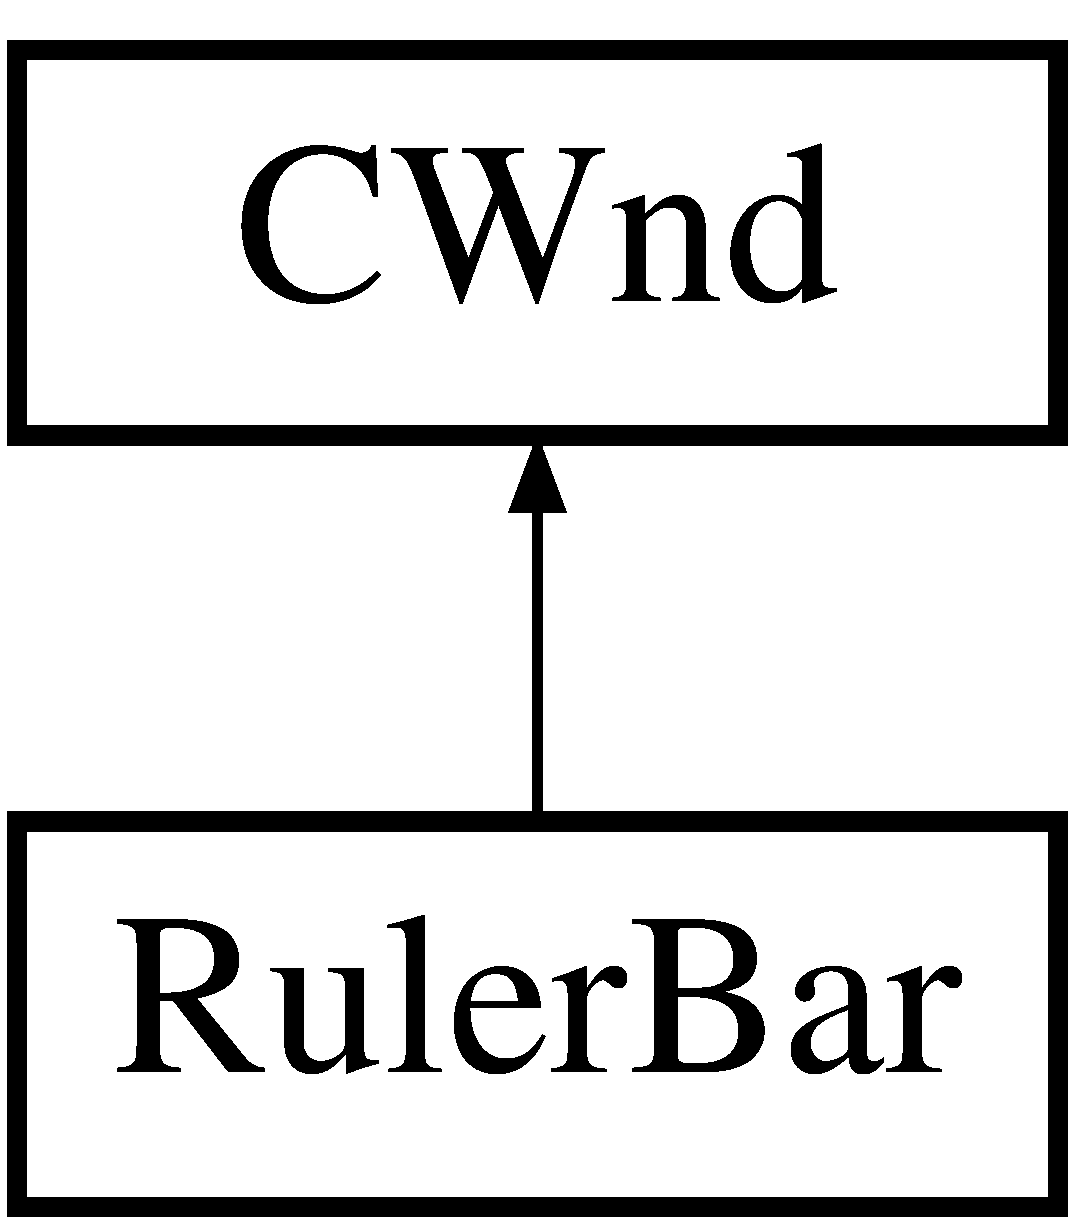
\includegraphics[height=2.000000cm]{class_ruler_bar}
\end{center}
\end{figure}
\subsection*{Public Member Functions}
\begin{DoxyCompactItemize}
\item 
\mbox{\Hypertarget{class_ruler_bar_ab7e5d9b49483974bfdf2b31f6312cbe5}\label{class_ruler_bar_ab7e5d9b49483974bfdf2b31f6312cbe5}} 
B\+O\+OL {\bfseries Create} (C\+Wnd $\ast$p\+Parent, B\+O\+OL b\+Type\+Horiz=T\+R\+UE)
\item 
\mbox{\Hypertarget{class_ruler_bar_adad01ca5e5ae6d994ede8d5cddd0f2ce}\label{class_ruler_bar_adad01ca5e5ae6d994ede8d5cddd0f2ce}} 
virtual B\+O\+OL {\bfseries Pre\+Create\+Window} (C\+R\+E\+A\+T\+E\+S\+T\+R\+U\+CT \&cs)
\item 
\mbox{\Hypertarget{class_ruler_bar_a6c403871b29483631af98fa4602fdfee}\label{class_ruler_bar_a6c403871b29483631af98fa4602fdfee}} 
afx\+\_\+msg void {\bfseries On\+Size} (U\+I\+NT n\+Type, int cx, int cy)
\item 
\mbox{\Hypertarget{class_ruler_bar_a09b55d38328a3cde6241aaba2d644809}\label{class_ruler_bar_a09b55d38328a3cde6241aaba2d644809}} 
afx\+\_\+msg int {\bfseries On\+Create} (L\+P\+C\+R\+E\+A\+T\+E\+S\+T\+R\+U\+CT lp\+Create\+Struct)
\item 
\mbox{\Hypertarget{class_ruler_bar_a24651900a15f82994bdb76198ccacf62}\label{class_ruler_bar_a24651900a15f82994bdb76198ccacf62}} 
afx\+\_\+msg void {\bfseries On\+Paint} ()
\end{DoxyCompactItemize}
\subsection*{Protected Attributes}
\begin{DoxyCompactItemize}
\item 
\mbox{\Hypertarget{class_ruler_bar_a41a7bf4f9af7375fb6304f7cdb69d2ed}\label{class_ruler_bar_a41a7bf4f9af7375fb6304f7cdb69d2ed}} 
B\+O\+OL {\bfseries m\+\_\+b\+Type\+Horiz}
\end{DoxyCompactItemize}


The documentation for this class was generated from the following files\+:\begin{DoxyCompactItemize}
\item 
i\+Optics/Ruler\+Bar.\+h\item 
i\+Optics/Ruler\+Bar.\+cpp\end{DoxyCompactItemize}

\hypertarget{class_ruler_corner}{}\section{Ruler\+Corner Class Reference}
\label{class_ruler_corner}\index{Ruler\+Corner@{Ruler\+Corner}}
Inheritance diagram for Ruler\+Corner\+:\begin{figure}[H]
\begin{center}
\leavevmode
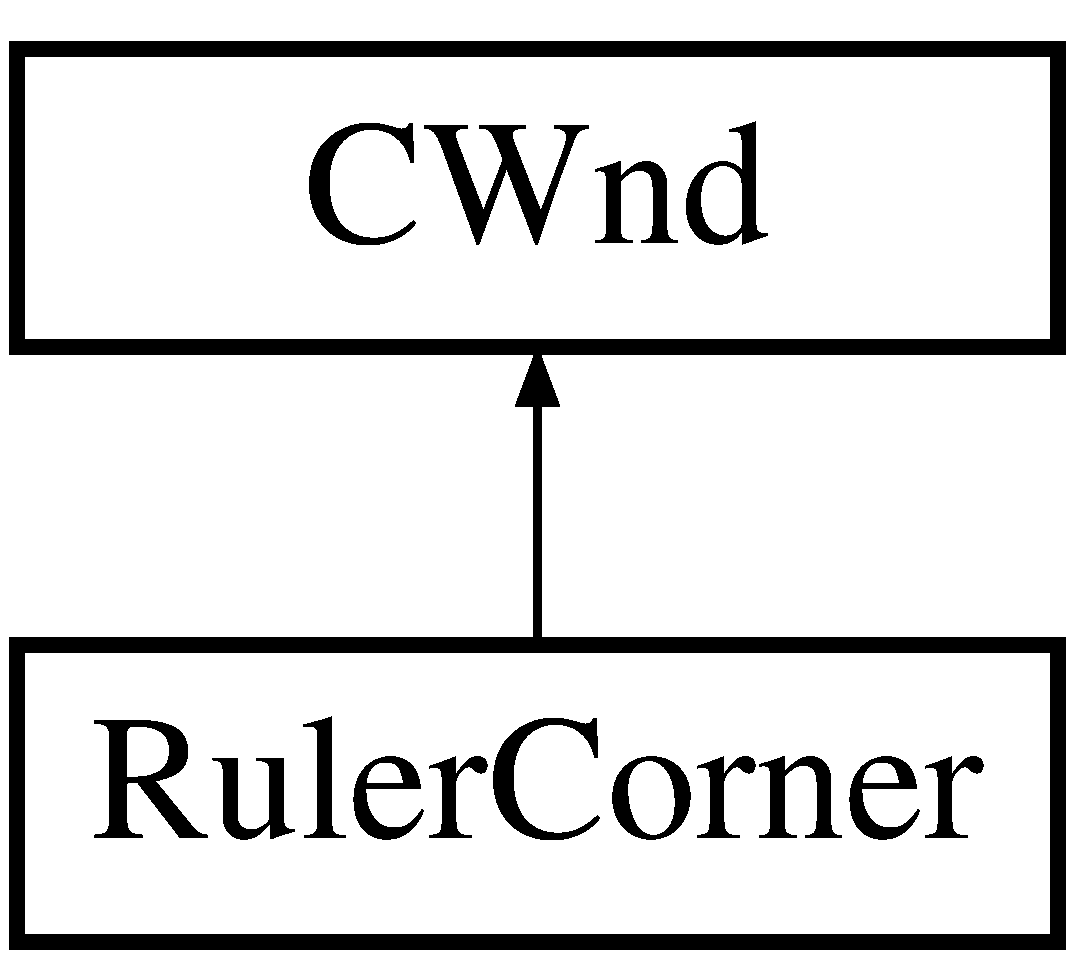
\includegraphics[height=2.000000cm]{class_ruler_corner}
\end{center}
\end{figure}
\subsection*{Public Member Functions}
\begin{DoxyCompactItemize}
\item 
\mbox{\Hypertarget{class_ruler_corner_a6f70a4658f3ea03d26c5ba424c58faa4}\label{class_ruler_corner_a6f70a4658f3ea03d26c5ba424c58faa4}} 
B\+O\+OL {\bfseries Create} (C\+Wnd $\ast$p\+Parent)
\item 
\mbox{\Hypertarget{class_ruler_corner_ac078b0f0fe0e57fc15dbf94b9c4178fe}\label{class_ruler_corner_ac078b0f0fe0e57fc15dbf94b9c4178fe}} 
virtual B\+O\+OL {\bfseries Pre\+Create\+Window} (C\+R\+E\+A\+T\+E\+S\+T\+R\+U\+CT \&cs)
\item 
\mbox{\Hypertarget{class_ruler_corner_ac9bf41b0ada5824789c42c4932487121}\label{class_ruler_corner_ac9bf41b0ada5824789c42c4932487121}} 
afx\+\_\+msg void {\bfseries On\+Paint} ()
\end{DoxyCompactItemize}


The documentation for this class was generated from the following files\+:\begin{DoxyCompactItemize}
\item 
i\+Optics/Ruler\+Bar.\+h\item 
i\+Optics/Ruler\+Bar.\+cpp\end{DoxyCompactItemize}

\hypertarget{class_work_view}{}\section{Work\+View Class Reference}
\label{class_work_view}\index{Work\+View@{Work\+View}}


\mbox{\hyperlink{class_work_view}{Work\+View}} is the current opened image display window. It can display gride and mesh for comparision with processed image. It also provides zooming and scrolling functions for viewing.  




{\ttfamily \#include $<$Work\+View.\+h$>$}

Inheritance diagram for Work\+View\+:\begin{figure}[H]
\begin{center}
\leavevmode
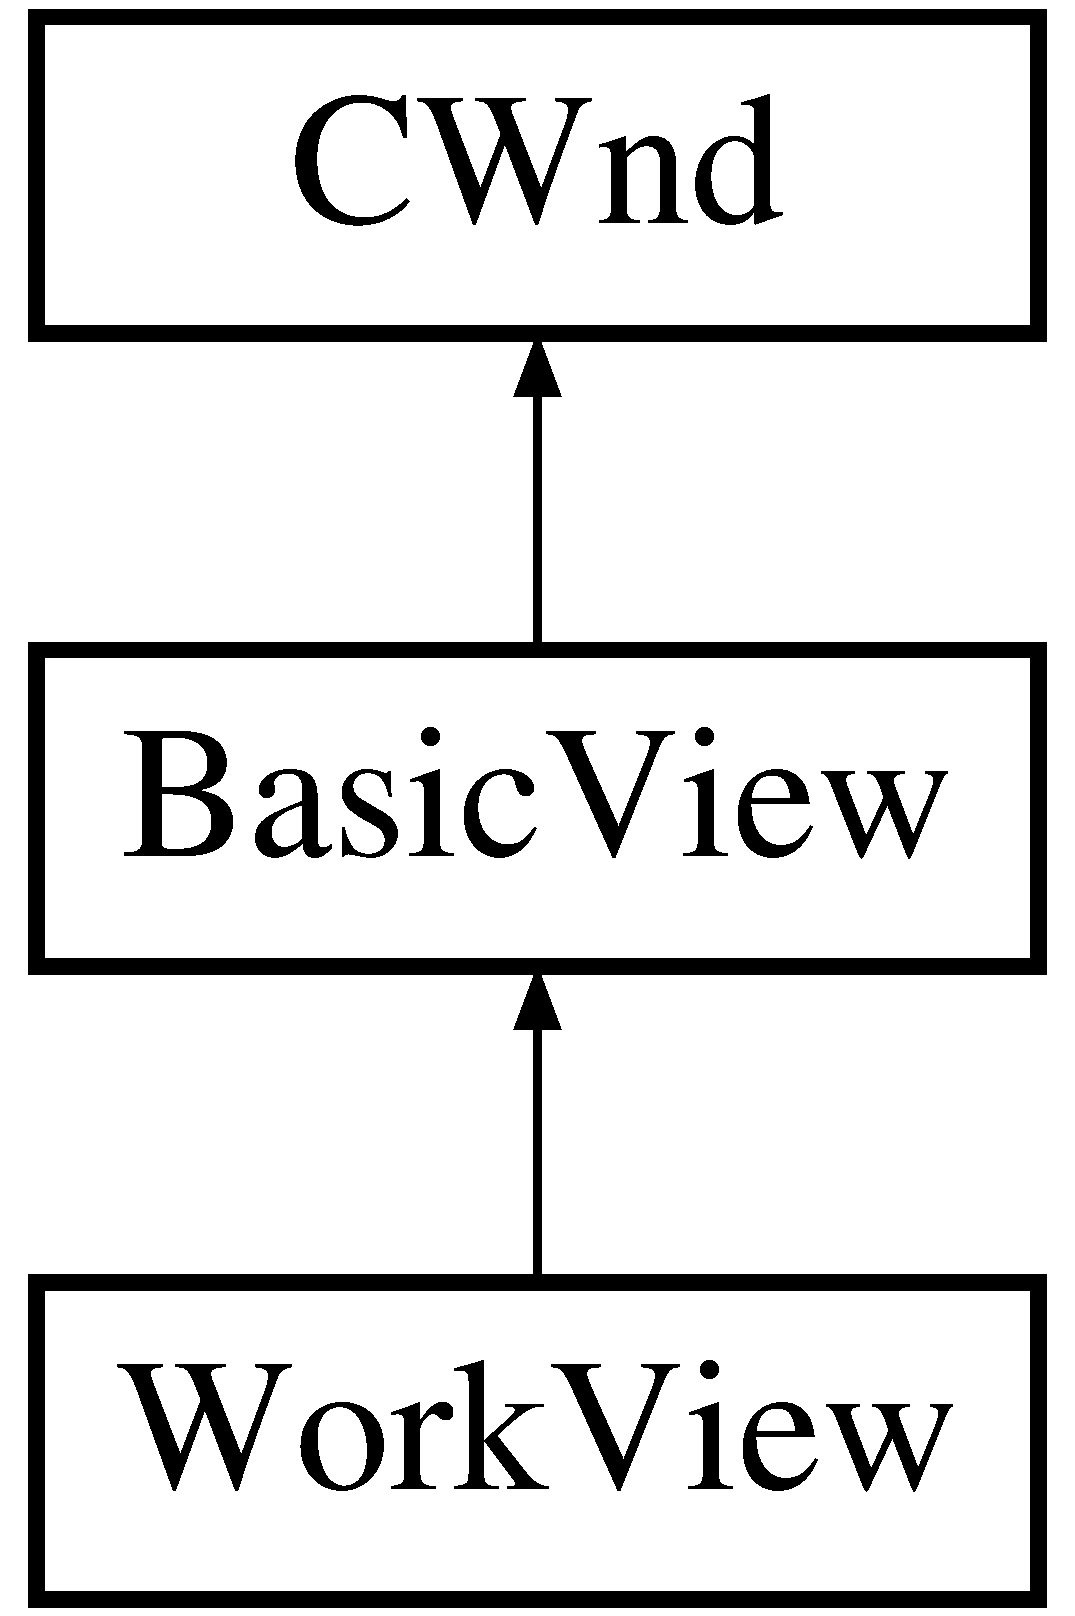
\includegraphics[height=3.000000cm]{class_work_view}
\end{center}
\end{figure}
\subsection*{Public Member Functions}
\begin{DoxyCompactItemize}
\item 
\mbox{\Hypertarget{class_work_view_a52d32e6dc47500c5146d54f4ba424fa2}\label{class_work_view_a52d32e6dc47500c5146d54f4ba424fa2}} 
B\+O\+OL {\bfseries Create} (C\+Wnd $\ast$p\+Parent)
\item 
\mbox{\Hypertarget{class_work_view_ac30e92784349602e62a91164d6527be9}\label{class_work_view_ac30e92784349602e62a91164d6527be9}} 
B\+O\+OL {\bfseries Set\+Scroll\+Pos} (int nX, int nY)
\item 
\mbox{\Hypertarget{class_work_view_a8926eb6da1d3b26cab931bb77cc89bbc}\label{class_work_view_a8926eb6da1d3b26cab931bb77cc89bbc}} 
virtual void {\bfseries Update\+Scrollbar\+Position} ()
\item 
\mbox{\Hypertarget{class_work_view_a0a258afb445a0c3233e898811c9b5723}\label{class_work_view_a0a258afb445a0c3233e898811c9b5723}} 
\mbox{\hyperlink{class_c_main_doc}{C\+Main\+Doc}} $\ast$ {\bfseries Get\+Document} ()
\item 
\mbox{\Hypertarget{class_work_view_aac149cb4e97f4067e350ff2df2f2e0bc}\label{class_work_view_aac149cb4e97f4067e350ff2df2f2e0bc}} 
Img\+File $\ast$ {\bfseries Get\+Image} ()
\item 
\mbox{\Hypertarget{class_work_view_ac396e13c1bf765c6add07386c3fc02c4}\label{class_work_view_ac396e13c1bf765c6add07386c3fc02c4}} 
virtual void {\bfseries On\+Update} (C\+View $\ast$p\+Sender, L\+P\+A\+R\+AM l\+Hint, C\+Object $\ast$p\+Hint)
\item 
\mbox{\Hypertarget{class_work_view_ae5fa678c052b3d9ac2dd6bc58d3210c8}\label{class_work_view_ae5fa678c052b3d9ac2dd6bc58d3210c8}} 
afx\+\_\+msg void {\bfseries On\+Size} (U\+I\+NT n\+Type, int cx, int cy)
\item 
\mbox{\Hypertarget{class_work_view_ae85f3de8ad0f27895e47f130630cea85}\label{class_work_view_ae85f3de8ad0f27895e47f130630cea85}} 
afx\+\_\+msg void {\bfseries On\+View\+Zoomin} ()
\item 
\mbox{\Hypertarget{class_work_view_ac2f07c79088ef99c6d5a90a377a8db6b}\label{class_work_view_ac2f07c79088ef99c6d5a90a377a8db6b}} 
afx\+\_\+msg void {\bfseries On\+Update\+View\+Zoomin} (C\+Cmd\+UI $\ast$p\+Cmd\+UI)
\item 
\mbox{\Hypertarget{class_work_view_a158434a846836afca5ba607102303951}\label{class_work_view_a158434a846836afca5ba607102303951}} 
afx\+\_\+msg void {\bfseries On\+View\+Zoomout} ()
\item 
\mbox{\Hypertarget{class_work_view_a25b12d323ee4b426bba4b738d6b60cb8}\label{class_work_view_a25b12d323ee4b426bba4b738d6b60cb8}} 
afx\+\_\+msg void {\bfseries On\+Update\+View\+Zoomout} (C\+Cmd\+UI $\ast$p\+Cmd\+UI)
\item 
\mbox{\Hypertarget{class_work_view_a3408bfe423d38af42731966bc6b1b5f8}\label{class_work_view_a3408bfe423d38af42731966bc6b1b5f8}} 
afx\+\_\+msg void {\bfseries On\+Mouse\+Move} (U\+I\+NT n\+Flags, C\+Point point)
\item 
\mbox{\Hypertarget{class_work_view_a251a6f512bd43f40a647517fb41eb68a}\label{class_work_view_a251a6f512bd43f40a647517fb41eb68a}} 
afx\+\_\+msg void {\bfseries On\+L\+Button\+Down} (U\+I\+NT n\+Flags, C\+Point point)
\item 
\mbox{\Hypertarget{class_work_view_ad66b49ccc4663eccbe9589a0754f9775}\label{class_work_view_ad66b49ccc4663eccbe9589a0754f9775}} 
afx\+\_\+msg void {\bfseries On\+L\+Button\+Up} (U\+I\+NT n\+Flags, C\+Point point)
\item 
\mbox{\Hypertarget{class_work_view_aa7974658428c358313f8c5578c89665d}\label{class_work_view_aa7974658428c358313f8c5578c89665d}} 
afx\+\_\+msg void {\bfseries On\+Destroy} ()
\item 
\mbox{\Hypertarget{class_work_view_affa363a468b358c178ab2feb5956c4e6}\label{class_work_view_affa363a468b358c178ab2feb5956c4e6}} 
afx\+\_\+msg int {\bfseries On\+Create} (L\+P\+C\+R\+E\+A\+T\+E\+S\+T\+R\+U\+CT lp\+Create\+Struct)
\item 
\mbox{\Hypertarget{class_work_view_acf3b77c19540468ff5b385dc1d3a05d7}\label{class_work_view_acf3b77c19540468ff5b385dc1d3a05d7}} 
afx\+\_\+msg void {\bfseries On\+Paint} ()
\item 
\mbox{\Hypertarget{class_work_view_a4eaa90a69961395efbfeaa4773e0588f}\label{class_work_view_a4eaa90a69961395efbfeaa4773e0588f}} 
afx\+\_\+msg void {\bfseries On\+View\+Gride} ()
\item 
\mbox{\Hypertarget{class_work_view_a86baee2b4009eea98833b3e98b352ae9}\label{class_work_view_a86baee2b4009eea98833b3e98b352ae9}} 
afx\+\_\+msg void {\bfseries On\+Update\+View\+Gride} (C\+Cmd\+UI $\ast$p\+Cmd\+UI)
\item 
\mbox{\Hypertarget{class_work_view_af3688036af8f371f405093e2f48fcc75}\label{class_work_view_af3688036af8f371f405093e2f48fcc75}} 
afx\+\_\+msg void {\bfseries On\+View\+Mesh} ()
\item 
\mbox{\Hypertarget{class_work_view_a9db7abfddac74a04efcf6a7249152965}\label{class_work_view_a9db7abfddac74a04efcf6a7249152965}} 
afx\+\_\+msg void {\bfseries On\+Update\+View\+Mesh} (C\+Cmd\+UI $\ast$p\+Cmd\+UI)
\item 
\mbox{\Hypertarget{class_work_view_ab1f8dafc5e94041874cab2efe9b1647a}\label{class_work_view_ab1f8dafc5e94041874cab2efe9b1647a}} 
afx\+\_\+msg void {\bfseries On\+Update\+Indicate\+Pos} (C\+Cmd\+UI $\ast$p\+Cmd\+UI)
\item 
\mbox{\Hypertarget{class_work_view_a02ab5b22f1df54d47048a3132a6be0eb}\label{class_work_view_a02ab5b22f1df54d47048a3132a6be0eb}} 
afx\+\_\+msg void {\bfseries On\+Update\+Indicate\+Color} (C\+Cmd\+UI $\ast$p\+Cmd\+UI)
\item 
\mbox{\Hypertarget{class_work_view_a7532947de83575c7930d2030245927be}\label{class_work_view_a7532947de83575c7930d2030245927be}} 
afx\+\_\+msg void {\bfseries On\+Update\+Indicate\+Zoom\+Factor} (C\+Cmd\+UI $\ast$p\+Cmd\+UI)
\item 
\mbox{\Hypertarget{class_work_view_a3b5e67652e2a38805d1f7733845b438c}\label{class_work_view_a3b5e67652e2a38805d1f7733845b438c}} 
afx\+\_\+msg void {\bfseries On\+Process\+Fec} ()
\item 
\mbox{\Hypertarget{class_work_view_a9dbcece36f66807285bcda9d74e18768}\label{class_work_view_a9dbcece36f66807285bcda9d74e18768}} 
afx\+\_\+msg void {\bfseries On\+Update\+Process\+Fec} (C\+Cmd\+UI $\ast$p\+Cmd\+UI)
\item 
\mbox{\Hypertarget{class_work_view_a2e21dab769506c6cbd2226c0e3afda3b}\label{class_work_view_a2e21dab769506c6cbd2226c0e3afda3b}} 
afx\+\_\+msg void {\bfseries On\+Process\+Ldc} ()
\item 
\mbox{\Hypertarget{class_work_view_afad796ba220493bff71a108948454d1b}\label{class_work_view_afad796ba220493bff71a108948454d1b}} 
afx\+\_\+msg void {\bfseries On\+Update\+Process\+Ldc} (C\+Cmd\+UI $\ast$p\+Cmd\+UI)
\item 
\mbox{\Hypertarget{class_work_view_a471b522ecb40aa8c9387faeca6955a5e}\label{class_work_view_a471b522ecb40aa8c9387faeca6955a5e}} 
afx\+\_\+msg void {\bfseries On\+Process\+Homo} ()
\item 
\mbox{\Hypertarget{class_work_view_aac95c904a9d4d6592b0aa8ffd7205545}\label{class_work_view_aac95c904a9d4d6592b0aa8ffd7205545}} 
afx\+\_\+msg void {\bfseries On\+Update\+Process\+Homo} (C\+Cmd\+UI $\ast$p\+Cmd\+UI)
\item 
\mbox{\Hypertarget{class_work_view_a3792019ca2113e37d5f890d73083e9a6}\label{class_work_view_a3792019ca2113e37d5f890d73083e9a6}} 
afx\+\_\+msg void {\bfseries On\+Process\+Exit} ()
\item 
\mbox{\Hypertarget{class_work_view_a4d3c4931b25cfdaf1068d8d3e40fd285}\label{class_work_view_a4d3c4931b25cfdaf1068d8d3e40fd285}} 
afx\+\_\+msg void {\bfseries On\+Toolbox\+Apply} ()
\item 
\mbox{\Hypertarget{class_work_view_a9a92da21e55e9f8a86bdf1100bc91047}\label{class_work_view_a9a92da21e55e9f8a86bdf1100bc91047}} 
afx\+\_\+msg void {\bfseries On\+Process\+Preview} ()
\item 
\mbox{\Hypertarget{class_work_view_a98b3f9ac9bea52d9bbc3e2ecaffdf78b}\label{class_work_view_a98b3f9ac9bea52d9bbc3e2ecaffdf78b}} 
afx\+\_\+msg void {\bfseries On\+Update\+Toolbox} (C\+Cmd\+UI $\ast$p\+Cmd\+UI)
\item 
\mbox{\Hypertarget{class_work_view_af3a6f050b573a4eb9c5dd1dc95cc7f68}\label{class_work_view_af3a6f050b573a4eb9c5dd1dc95cc7f68}} 
afx\+\_\+msg void {\bfseries On\+Command\+Toolbox} (U\+I\+NT n\+Cmd)
\end{DoxyCompactItemize}
\subsection*{Public Attributes}
\begin{DoxyCompactItemize}
\item 
P\+O\+I\+NT \mbox{\hyperlink{class_work_view_ac4c6b3ea30ed20afd8fc96dc9be9a5b6}{m\+\_\+pt\+Cursor\+Pos}}
\end{DoxyCompactItemize}
\subsection*{Protected Member Functions}
\begin{DoxyCompactItemize}
\item 
\mbox{\Hypertarget{class_work_view_a66b822a6f10fe9b452faa3d1675cc3d4}\label{class_work_view_a66b822a6f10fe9b452faa3d1675cc3d4}} 
virtual B\+O\+OL {\bfseries On\+Command} (W\+P\+A\+R\+AM w\+Param, L\+P\+A\+R\+AM l\+Param)
\end{DoxyCompactItemize}
\subsection*{Protected Attributes}
\begin{DoxyCompactItemize}
\item 
\mbox{\Hypertarget{class_work_view_aa9e63e4f5c106048c266408640295045}\label{class_work_view_aa9e63e4f5c106048c266408640295045}} 
\mbox{\hyperlink{class_c_main_view}{C\+Main\+View}} $\ast$ {\bfseries m\+\_\+parent}
\item 
\mbox{\hyperlink{class_process_tool}{Process\+Tool}} $\ast$ \mbox{\hyperlink{class_work_view_ae70044302a41f2ad4315159eb07c6451}{m\+\_\+p\+Process\+Tool}}
\item 
\mbox{\Hypertarget{class_work_view_a22980da53a224fb6bc98fd1761196561}\label{class_work_view_a22980da53a224fb6bc98fd1761196561}} 
B\+O\+OL {\bfseries m\+\_\+b\+Show\+Gride}
\item 
\mbox{\Hypertarget{class_work_view_a684a8e103025c104c7b39c1c26e5a5b3}\label{class_work_view_a684a8e103025c104c7b39c1c26e5a5b3}} 
\mbox{\hyperlink{class_gride}{Gride}} {\bfseries m\+\_\+gride}
\item 
\mbox{\hyperlink{class_gride}{Gride}} $\ast$ \mbox{\hyperlink{class_work_view_a9e286bc84a23735521f04f1c93598a07}{m\+\_\+p\+Tool\+Gride}}
\item 
\mbox{\Hypertarget{class_work_view_a6ffb988df047900be9e1281a1a322c96}\label{class_work_view_a6ffb988df047900be9e1281a1a322c96}} 
B\+O\+OL {\bfseries m\+\_\+b\+Show\+Mesh}
\item 
\mbox{\hyperlink{class_mesh}{Mesh}} \mbox{\hyperlink{class_work_view_a75b75053528bcfe74fc2805fd723bc05}{m\+\_\+mesh}}
\end{DoxyCompactItemize}
\subsection*{Additional Inherited Members}


\subsection{Detailed Description}
\mbox{\hyperlink{class_work_view}{Work\+View}} is the current opened image display window. It can display gride and mesh for comparision with processed image. It also provides zooming and scrolling functions for viewing. 

\subsection{Member Data Documentation}
\mbox{\Hypertarget{class_work_view_a75b75053528bcfe74fc2805fd723bc05}\label{class_work_view_a75b75053528bcfe74fc2805fd723bc05}} 
\index{Work\+View@{Work\+View}!m\+\_\+mesh@{m\+\_\+mesh}}
\index{m\+\_\+mesh@{m\+\_\+mesh}!Work\+View@{Work\+View}}
\subsubsection{\texorpdfstring{m\+\_\+mesh}{m\_mesh}}
{\footnotesize\ttfamily \mbox{\hyperlink{class_mesh}{Mesh}} Work\+View\+::m\+\_\+mesh\hspace{0.3cm}{\ttfamily [protected]}}

mesh control class \mbox{\Hypertarget{class_work_view_ae70044302a41f2ad4315159eb07c6451}\label{class_work_view_ae70044302a41f2ad4315159eb07c6451}} 
\index{Work\+View@{Work\+View}!m\+\_\+p\+Process\+Tool@{m\+\_\+p\+Process\+Tool}}
\index{m\+\_\+p\+Process\+Tool@{m\+\_\+p\+Process\+Tool}!Work\+View@{Work\+View}}
\subsubsection{\texorpdfstring{m\+\_\+p\+Process\+Tool}{m\_pProcessTool}}
{\footnotesize\ttfamily \mbox{\hyperlink{class_process_tool}{Process\+Tool}}$\ast$ Work\+View\+::m\+\_\+p\+Process\+Tool\hspace{0.3cm}{\ttfamily [protected]}}

pointer to current process control dialog box \mbox{\Hypertarget{class_work_view_ac4c6b3ea30ed20afd8fc96dc9be9a5b6}\label{class_work_view_ac4c6b3ea30ed20afd8fc96dc9be9a5b6}} 
\index{Work\+View@{Work\+View}!m\+\_\+pt\+Cursor\+Pos@{m\+\_\+pt\+Cursor\+Pos}}
\index{m\+\_\+pt\+Cursor\+Pos@{m\+\_\+pt\+Cursor\+Pos}!Work\+View@{Work\+View}}
\subsubsection{\texorpdfstring{m\+\_\+pt\+Cursor\+Pos}{m\_ptCursorPos}}
{\footnotesize\ttfamily P\+O\+I\+NT Work\+View\+::m\+\_\+pt\+Cursor\+Pos}

current cursor position on original image \mbox{\Hypertarget{class_work_view_a9e286bc84a23735521f04f1c93598a07}\label{class_work_view_a9e286bc84a23735521f04f1c93598a07}} 
\index{Work\+View@{Work\+View}!m\+\_\+p\+Tool\+Gride@{m\+\_\+p\+Tool\+Gride}}
\index{m\+\_\+p\+Tool\+Gride@{m\+\_\+p\+Tool\+Gride}!Work\+View@{Work\+View}}
\subsubsection{\texorpdfstring{m\+\_\+p\+Tool\+Gride}{m\_pToolGride}}
{\footnotesize\ttfamily \mbox{\hyperlink{class_gride}{Gride}}$\ast$ Work\+View\+::m\+\_\+p\+Tool\+Gride\hspace{0.3cm}{\ttfamily [protected]}}

gride line for the selected processing tool 

The documentation for this class was generated from the following files\+:\begin{DoxyCompactItemize}
\item 
i\+Optics/\mbox{\hyperlink{_work_view_8h}{Work\+View.\+h}}\item 
i\+Optics/Work\+View.\+cpp\end{DoxyCompactItemize}

\chapter{File Documentation}
\hypertarget{_basic_view_8h}{}\section{i\+Optics/\+Basic\+View.h File Reference}
\label{_basic_view_8h}\index{i\+Optics/\+Basic\+View.\+h@{i\+Optics/\+Basic\+View.\+h}}
\subsection*{Classes}
\begin{DoxyCompactItemize}
\item 
class \mbox{\hyperlink{class_basic_view}{Basic\+View}}
\begin{DoxyCompactList}\small\item\em \mbox{\hyperlink{class_basic_view}{Basic\+View}} is the basic image viewer window. It handles image preview, zoom in/out, and window scrolling stuff. \end{DoxyCompactList}\end{DoxyCompactItemize}
\subsection*{Macros}
\begin{DoxyCompactItemize}
\item 
\mbox{\Hypertarget{_basic_view_8h_a5ccab1c5a5148810372b1aa049a6397d}\label{_basic_view_8h_a5ccab1c5a5148810372b1aa049a6397d}} 
\#define {\bfseries M\+A\+X\+\_\+\+Z\+O\+OM}~10
\item 
\mbox{\Hypertarget{_basic_view_8h_aff49c43019a5897017348821545ddcee}\label{_basic_view_8h_aff49c43019a5897017348821545ddcee}} 
\#define {\bfseries D\+E\+F\+A\+U\+L\+T\+\_\+\+Z\+O\+O\+M\+\_\+\+F\+A\+C\+T\+OR}~5
\end{DoxyCompactItemize}


\subsection{Detailed Description}
declarations of class \mbox{\hyperlink{class_basic_view}{Basic\+View}} 
\hypertarget{common_8h}{}\section{i\+Optics/common.h File Reference}
\label{common_8h}\index{i\+Optics/common.\+h@{i\+Optics/common.\+h}}


This file declars process-\/related struc and data type.  


\subsection*{Classes}
\begin{DoxyCompactItemize}
\item 
struct \mbox{\hyperlink{struct___point_double}{\+\_\+\+Point\+Double}}
\begin{DoxyCompactList}\small\item\em double precision types of position coordinates used in L\+UT \end{DoxyCompactList}\item 
struct \mbox{\hyperlink{struct___fec_param}{\+\_\+\+Fec\+Param}}
\begin{DoxyCompactList}\small\item\em F\+EC processing parameters. \end{DoxyCompactList}\item 
struct \mbox{\hyperlink{struct___homo_param}{\+\_\+\+Homo\+Param}}
\begin{DoxyCompactList}\small\item\em Homography Matrix parameters. Q(u,v) = \mbox{[}H\mbox{]} $\ast$ P(x,y), where P is the vector of original pixels, Q is the vector of transformed pixels. \end{DoxyCompactList}\end{DoxyCompactItemize}
\subsection*{Macros}
\begin{DoxyCompactItemize}
\item 
\mbox{\Hypertarget{common_8h_a916e92ae9237b31e838e362c5e75ab51}\label{common_8h_a916e92ae9237b31e838e362c5e75ab51}} 
\#define {\bfseries C\+L\+IP}(x)~min(255, max(0,x))
\item 
\mbox{\Hypertarget{common_8h_a598a3330b3c21701223ee0ca14316eca}\label{common_8h_a598a3330b3c21701223ee0ca14316eca}} 
\#define {\bfseries PI}~3.\+14159265358979323846f /$\ast$ pi $\ast$/
\item 
\mbox{\Hypertarget{common_8h_a7c7671235d3f0d09bc5c011920fe0d5b}\label{common_8h_a7c7671235d3f0d09bc5c011920fe0d5b}} 
\#define {\bfseries P\+I\+\_\+2}~1.\+57079632679489661923f /$\ast$ pi/2 $\ast$/
\end{DoxyCompactItemize}
\subsection*{Typedefs}
\begin{DoxyCompactItemize}
\item 
\mbox{\Hypertarget{common_8h_aa960c1131ba75a7afd8877c2a1c7b238}\label{common_8h_aa960c1131ba75a7afd8877c2a1c7b238}} 
typedef struct \mbox{\hyperlink{struct___point_double}{\+\_\+\+Point\+Double}} {\bfseries Point\+Double}
\item 
\mbox{\Hypertarget{common_8h_a13b907420152fb8bd1de1482ebba2b03}\label{common_8h_a13b907420152fb8bd1de1482ebba2b03}} 
typedef enum \mbox{\hyperlink{common_8h_a4493c1033486227a5340672c32384eda}{\+\_\+\+Mount\+Mode}} {\bfseries Mount\+Mode}
\item 
\mbox{\Hypertarget{common_8h_a3a73d064a8538a6f7c4239a71b517d6e}\label{common_8h_a3a73d064a8538a6f7c4239a71b517d6e}} 
typedef enum \mbox{\hyperlink{common_8h_ac251312fa48af25715d391f384b78be7}{\+\_\+\+Lens\+Type}} {\bfseries Lens\+Type}
\item 
\mbox{\Hypertarget{common_8h_a82fa6e4dc23f551122da509b0ed8bacb}\label{common_8h_a82fa6e4dc23f551122da509b0ed8bacb}} 
typedef struct \mbox{\hyperlink{struct___fec_param}{\+\_\+\+Fec\+Param}} {\bfseries Fec\+Param}
\item 
\mbox{\Hypertarget{common_8h_a39063049f8cb0a595d5271e6832cd1fe}\label{common_8h_a39063049f8cb0a595d5271e6832cd1fe}} 
typedef struct \mbox{\hyperlink{struct___homo_param}{\+\_\+\+Homo\+Param}} {\bfseries Homo\+Param}
\end{DoxyCompactItemize}
\subsection*{Enumerations}
\begin{DoxyCompactItemize}
\item 
enum \mbox{\hyperlink{common_8h_a4493c1033486227a5340672c32384eda}{\+\_\+\+Mount\+Mode}} \{ \mbox{\hyperlink{common_8h_a4493c1033486227a5340672c32384edaafd0a6f0b9be724fddb3cb101edacacde}{Mount\+Mode\+\_\+\+W\+A\+LL}} = 0, 
\mbox{\hyperlink{common_8h_a4493c1033486227a5340672c32384edaaabf9054e23c9d38482238add78c9b2c4}{Mount\+Mode\+\_\+\+C\+E\+I\+L\+I\+NG}} = 1, 
\mbox{\hyperlink{common_8h_a4493c1033486227a5340672c32384edaa86b32e48aba9f304809ba9ada97c7542}{Mount\+Mode\+\_\+\+T\+A\+B\+LE}} = 2
 \}
\begin{DoxyCompactList}\small\item\em camera mounting position \end{DoxyCompactList}\item 
enum \mbox{\hyperlink{common_8h_ac251312fa48af25715d391f384b78be7}{\+\_\+\+Lens\+Type}} \{ \newline
\mbox{\hyperlink{common_8h_ac251312fa48af25715d391f384b78be7a9fb7343a9809d42474e503898c152165}{Lens\+Type\+\_\+0}}, 
\mbox{\hyperlink{common_8h_ac251312fa48af25715d391f384b78be7a13954ac30fe273506a2cb0ca6b85bd20}{Lens\+Type\+\_\+1}}, 
\mbox{\hyperlink{common_8h_ac251312fa48af25715d391f384b78be7a641c46a975322bcc7ac720b202bc1ed0}{Lens\+Type\+\_\+2}}, 
\mbox{\hyperlink{common_8h_ac251312fa48af25715d391f384b78be7a909c2a26cfadb53f5e08925d633db945}{Lens\+Type\+\_\+3}}, 
\newline
\mbox{\hyperlink{common_8h_ac251312fa48af25715d391f384b78be7a3336f117afd63125fcb79ea01010b2d3}{Lens\+Type\+\_\+4}}, 
\mbox{\hyperlink{common_8h_ac251312fa48af25715d391f384b78be7addaf12b4ef4cce1a3a78166a5b8c3091}{Lens\+Type\+\_\+5}}
 \}
\begin{DoxyCompactList}\small\item\em defines lens distortion model \end{DoxyCompactList}\end{DoxyCompactItemize}


\subsection{Detailed Description}
This file declars process-\/related struc and data type. 



\subsection{Enumeration Type Documentation}
\mbox{\Hypertarget{common_8h_ac251312fa48af25715d391f384b78be7}\label{common_8h_ac251312fa48af25715d391f384b78be7}} 
\index{common.\+h@{common.\+h}!\+\_\+\+Lens\+Type@{\+\_\+\+Lens\+Type}}
\index{\+\_\+\+Lens\+Type@{\+\_\+\+Lens\+Type}!common.\+h@{common.\+h}}
\subsubsection{\texorpdfstring{\+\_\+\+Lens\+Type}{\_LensType}}
{\footnotesize\ttfamily enum \mbox{\hyperlink{common_8h_ac251312fa48af25715d391f384b78be7}{\+\_\+\+Lens\+Type}}}



defines lens distortion model 

\begin{DoxyEnumFields}{Enumerator}
\raisebox{\heightof{T}}[0pt][0pt]{\index{Lens\+Type\+\_\+0@{Lens\+Type\+\_\+0}!common.\+h@{common.\+h}}\index{common.\+h@{common.\+h}!Lens\+Type\+\_\+0@{Lens\+Type\+\_\+0}}}\mbox{\Hypertarget{common_8h_ac251312fa48af25715d391f384b78be7a9fb7343a9809d42474e503898c152165}\label{common_8h_ac251312fa48af25715d391f384b78be7a9fb7343a9809d42474e503898c152165}} 
Lens\+Type\+\_\+0&no correction \\
\hline

\raisebox{\heightof{T}}[0pt][0pt]{\index{Lens\+Type\+\_\+1@{Lens\+Type\+\_\+1}!common.\+h@{common.\+h}}\index{common.\+h@{common.\+h}!Lens\+Type\+\_\+1@{Lens\+Type\+\_\+1}}}\mbox{\Hypertarget{common_8h_ac251312fa48af25715d391f384b78be7a13954ac30fe273506a2cb0ca6b85bd20}\label{common_8h_ac251312fa48af25715d391f384b78be7a13954ac30fe273506a2cb0ca6b85bd20}} 
Lens\+Type\+\_\+1&tan(angle/2) \\
\hline

\raisebox{\heightof{T}}[0pt][0pt]{\index{Lens\+Type\+\_\+2@{Lens\+Type\+\_\+2}!common.\+h@{common.\+h}}\index{common.\+h@{common.\+h}!Lens\+Type\+\_\+2@{Lens\+Type\+\_\+2}}}\mbox{\Hypertarget{common_8h_ac251312fa48af25715d391f384b78be7a641c46a975322bcc7ac720b202bc1ed0}\label{common_8h_ac251312fa48af25715d391f384b78be7a641c46a975322bcc7ac720b202bc1ed0}} 
Lens\+Type\+\_\+2&sin(angle/2) \\
\hline

\raisebox{\heightof{T}}[0pt][0pt]{\index{Lens\+Type\+\_\+3@{Lens\+Type\+\_\+3}!common.\+h@{common.\+h}}\index{common.\+h@{common.\+h}!Lens\+Type\+\_\+3@{Lens\+Type\+\_\+3}}}\mbox{\Hypertarget{common_8h_ac251312fa48af25715d391f384b78be7a909c2a26cfadb53f5e08925d633db945}\label{common_8h_ac251312fa48af25715d391f384b78be7a909c2a26cfadb53f5e08925d633db945}} 
Lens\+Type\+\_\+3&angle \\
\hline

\raisebox{\heightof{T}}[0pt][0pt]{\index{Lens\+Type\+\_\+4@{Lens\+Type\+\_\+4}!common.\+h@{common.\+h}}\index{common.\+h@{common.\+h}!Lens\+Type\+\_\+4@{Lens\+Type\+\_\+4}}}\mbox{\Hypertarget{common_8h_ac251312fa48af25715d391f384b78be7a3336f117afd63125fcb79ea01010b2d3}\label{common_8h_ac251312fa48af25715d391f384b78be7a3336f117afd63125fcb79ea01010b2d3}} 
Lens\+Type\+\_\+4&sin(angle) \\
\hline

\raisebox{\heightof{T}}[0pt][0pt]{\index{Lens\+Type\+\_\+5@{Lens\+Type\+\_\+5}!common.\+h@{common.\+h}}\index{common.\+h@{common.\+h}!Lens\+Type\+\_\+5@{Lens\+Type\+\_\+5}}}\mbox{\Hypertarget{common_8h_ac251312fa48af25715d391f384b78be7addaf12b4ef4cce1a3a78166a5b8c3091}\label{common_8h_ac251312fa48af25715d391f384b78be7addaf12b4ef4cce1a3a78166a5b8c3091}} 
Lens\+Type\+\_\+5&user defined curve \\
\hline

\end{DoxyEnumFields}
\mbox{\Hypertarget{common_8h_a4493c1033486227a5340672c32384eda}\label{common_8h_a4493c1033486227a5340672c32384eda}} 
\index{common.\+h@{common.\+h}!\+\_\+\+Mount\+Mode@{\+\_\+\+Mount\+Mode}}
\index{\+\_\+\+Mount\+Mode@{\+\_\+\+Mount\+Mode}!common.\+h@{common.\+h}}
\subsubsection{\texorpdfstring{\+\_\+\+Mount\+Mode}{\_MountMode}}
{\footnotesize\ttfamily enum \mbox{\hyperlink{common_8h_a4493c1033486227a5340672c32384eda}{\+\_\+\+Mount\+Mode}}}



camera mounting position 

\begin{DoxyEnumFields}{Enumerator}
\raisebox{\heightof{T}}[0pt][0pt]{\index{Mount\+Mode\+\_\+\+W\+A\+LL@{Mount\+Mode\+\_\+\+W\+A\+LL}!common.\+h@{common.\+h}}\index{common.\+h@{common.\+h}!Mount\+Mode\+\_\+\+W\+A\+LL@{Mount\+Mode\+\_\+\+W\+A\+LL}}}\mbox{\Hypertarget{common_8h_a4493c1033486227a5340672c32384edaafd0a6f0b9be724fddb3cb101edacacde}\label{common_8h_a4493c1033486227a5340672c32384edaafd0a6f0b9be724fddb3cb101edacacde}} 
Mount\+Mode\+\_\+\+W\+A\+LL&on the wall, only support this \\
\hline

\raisebox{\heightof{T}}[0pt][0pt]{\index{Mount\+Mode\+\_\+\+C\+E\+I\+L\+I\+NG@{Mount\+Mode\+\_\+\+C\+E\+I\+L\+I\+NG}!common.\+h@{common.\+h}}\index{common.\+h@{common.\+h}!Mount\+Mode\+\_\+\+C\+E\+I\+L\+I\+NG@{Mount\+Mode\+\_\+\+C\+E\+I\+L\+I\+NG}}}\mbox{\Hypertarget{common_8h_a4493c1033486227a5340672c32384edaaabf9054e23c9d38482238add78c9b2c4}\label{common_8h_a4493c1033486227a5340672c32384edaaabf9054e23c9d38482238add78c9b2c4}} 
Mount\+Mode\+\_\+\+C\+E\+I\+L\+I\+NG&on celling, not support yet \\
\hline

\raisebox{\heightof{T}}[0pt][0pt]{\index{Mount\+Mode\+\_\+\+T\+A\+B\+LE@{Mount\+Mode\+\_\+\+T\+A\+B\+LE}!common.\+h@{common.\+h}}\index{common.\+h@{common.\+h}!Mount\+Mode\+\_\+\+T\+A\+B\+LE@{Mount\+Mode\+\_\+\+T\+A\+B\+LE}}}\mbox{\Hypertarget{common_8h_a4493c1033486227a5340672c32384edaa86b32e48aba9f304809ba9ada97c7542}\label{common_8h_a4493c1033486227a5340672c32384edaa86b32e48aba9f304809ba9ada97c7542}} 
Mount\+Mode\+\_\+\+T\+A\+B\+LE&on table, not support yet \\
\hline

\end{DoxyEnumFields}

\hypertarget{_fec_tool_8h}{}\section{i\+Optics/\+Fec\+Tool.h File Reference}
\label{_fec_tool_8h}\index{i\+Optics/\+Fec\+Tool.\+h@{i\+Optics/\+Fec\+Tool.\+h}}
{\ttfamily \#include \char`\"{}common.\+h\char`\"{}}\newline
{\ttfamily \#include \char`\"{}Process\+Tool.\+h\char`\"{}}\newline
\subsection*{Classes}
\begin{DoxyCompactItemize}
\item 
class \mbox{\hyperlink{class_fec_wrap}{Fec\+Wrap}}
\begin{DoxyCompactList}\small\item\em F\+EC process parameters wrapper This class wrap F\+EC parameters and L\+UT table, as well as L\+UT generating function. \end{DoxyCompactList}\item 
class \mbox{\hyperlink{class_fec_tool}{Fec\+Tool}}
\begin{DoxyCompactList}\small\item\em \mbox{\hyperlink{class_fec_tool}{Fec\+Tool}} is used to control the settings of F\+EC process with UI in a dialog box. This class sends the parameters to a \mbox{\hyperlink{class_fec_view}{Fec\+View}} to display the resulted image. It also connects to a \mbox{\hyperlink{class_fec_wrap}{Fec\+Wrap}} class to maintain the F\+EC process related parameters and L\+UT data. \end{DoxyCompactList}\end{DoxyCompactItemize}


\subsection{Detailed Description}
declarations of class \mbox{\hyperlink{class_fec_tool}{Fec\+Tool}} and \mbox{\hyperlink{class_fec_wrap}{Fec\+Wrap}} 
\hypertarget{_fec_view_8h}{}\section{i\+Optics/\+Fec\+View.h File Reference}
\label{_fec_view_8h}\index{i\+Optics/\+Fec\+View.\+h@{i\+Optics/\+Fec\+View.\+h}}
{\ttfamily \#include \char`\"{}Process\+View.\+h\char`\"{}}\newline
{\ttfamily \#include \char`\"{}Fec\+Tool.\+h\char`\"{}}\newline
\subsection*{Classes}
\begin{DoxyCompactItemize}
\item 
class \mbox{\hyperlink{class_fec_view}{Fec\+View}}
\begin{DoxyCompactList}\small\item\em \mbox{\hyperlink{class_fec_view}{Fec\+View}} is the image viewer for F\+EC processing image. It handles the video rendering process by the specified process. It is controlled by its process correspondent \mbox{\hyperlink{class_fec_tool}{Fec\+Tool}}. It also can display gride lines on the image window. \end{DoxyCompactList}\end{DoxyCompactItemize}


\subsection{Detailed Description}
declarations of class \mbox{\hyperlink{class_fec_view}{Fec\+View}} 
\hypertarget{_homo_view_8h}{}\section{i\+Optics/\+Homo\+View.h File Reference}
\label{_homo_view_8h}\index{i\+Optics/\+Homo\+View.\+h@{i\+Optics/\+Homo\+View.\+h}}
{\ttfamily \#include \char`\"{}Process\+View.\+h\char`\"{}}\newline
{\ttfamily \#include \char`\"{}Homo\+Tool.\+h\char`\"{}}\newline
\subsection*{Classes}
\begin{DoxyCompactItemize}
\item 
class \mbox{\hyperlink{class_homo_view}{Homo\+View}}
\begin{DoxyCompactList}\small\item\em \mbox{\hyperlink{class_homo_view}{Homo\+View}} is the image viewer for Homography matrix processing image. It handles the video rendering process by the specified process. It is controlled by its process correspondent \mbox{\hyperlink{class_homo_tool}{Homo\+Tool}}. It also can display gride lines on the image window. \end{DoxyCompactList}\end{DoxyCompactItemize}


\subsection{Detailed Description}
declarations of class \mbox{\hyperlink{class_homo_view}{Homo\+View}} 
\hypertarget{_ldc_tool_8h}{}\section{i\+Optics/\+Ldc\+Tool.h File Reference}
\label{_ldc_tool_8h}\index{i\+Optics/\+Ldc\+Tool.\+h@{i\+Optics/\+Ldc\+Tool.\+h}}
{\ttfamily \#include \char`\"{}common.\+h\char`\"{}}\newline
{\ttfamily \#include \char`\"{}Process\+Tool.\+h\char`\"{}}\newline
\subsection*{Classes}
\begin{DoxyCompactItemize}
\item 
class \mbox{\hyperlink{class_ldc_wrap}{Ldc\+Wrap}}
\begin{DoxyCompactList}\small\item\em L\+DC process parameters wrapper This class wrap L\+DC parameters and L\+UT table, as well as L\+UT generating function. \end{DoxyCompactList}\item 
class \mbox{\hyperlink{class_ldc_tool}{Ldc\+Tool}}
\begin{DoxyCompactList}\small\item\em Ldcc\+Tool is used to control the settings of Ldc process with UI in a dialog box. This class sends the parameters to a \mbox{\hyperlink{class_fec_view}{Fec\+View}} to display the resulted image. It also connects to a \mbox{\hyperlink{class_ldc_wrap}{Ldc\+Wrap}} class to maintain the L\+DC process related parameters and L\+UT data. \end{DoxyCompactList}\end{DoxyCompactItemize}


\subsection{Detailed Description}
declarations of class \mbox{\hyperlink{class_ldc_tool}{Ldc\+Tool}} and \mbox{\hyperlink{class_ldc_wrap}{Ldc\+Wrap}} 
\hypertarget{_ldc_view_8h}{}\section{i\+Optics/\+Ldc\+View.h File Reference}
\label{_ldc_view_8h}\index{i\+Optics/\+Ldc\+View.\+h@{i\+Optics/\+Ldc\+View.\+h}}
{\ttfamily \#include \char`\"{}Process\+View.\+h\char`\"{}}\newline
{\ttfamily \#include \char`\"{}Ldc\+Tool.\+h\char`\"{}}\newline
\subsection*{Classes}
\begin{DoxyCompactItemize}
\item 
class \mbox{\hyperlink{class_ldc_view}{Ldc\+View}}
\begin{DoxyCompactList}\small\item\em \mbox{\hyperlink{class_ldc_view}{Ldc\+View}} is the image viewer for L\+DC processing image. It handles the video rendering process by the specified process. It is controlled by its process correspondent \mbox{\hyperlink{class_ldc_tool}{Ldc\+Tool}}. It also can display gride lines on the image window. \end{DoxyCompactList}\end{DoxyCompactItemize}


\subsection{Detailed Description}
declarations of class \mbox{\hyperlink{class_ldc_view}{Ldc\+View}} 
\hypertarget{_mesh_8cpp}{}\section{i\+Optics/\+Mesh.cpp File Reference}
\label{_mesh_8cpp}\index{i\+Optics/\+Mesh.\+cpp@{i\+Optics/\+Mesh.\+cpp}}


\mbox{\hyperlink{class_mesh}{Mesh}} is used to draw look-\/up table of image transformation, as mesh like, on an image.  


{\ttfamily \#include \char`\"{}stdafx.\+h\char`\"{}}\newline
{\ttfamily \#include \char`\"{}Mesh.\+h\char`\"{}}\newline
\subsection*{Macros}
\begin{DoxyCompactItemize}
\item 
\mbox{\Hypertarget{_mesh_8cpp_a248b045e54422372845d40c1da36cc9f}\label{_mesh_8cpp_a248b045e54422372845d40c1da36cc9f}} 
\#define {\bfseries C\+P\+\_\+\+S\+I\+ZE}~3
\item 
\mbox{\Hypertarget{_mesh_8cpp_a741717e9874693c89af2335a1b36557d}\label{_mesh_8cpp_a741717e9874693c89af2335a1b36557d}} 
\#define {\bfseries C\+P\+\_\+\+C\+O\+L\+OR}~R\+GB(255,255,255)
\item 
\mbox{\Hypertarget{_mesh_8cpp_af07f0b9d220b9aa8bccc2bd34bd3f368}\label{_mesh_8cpp_af07f0b9d220b9aa8bccc2bd34bd3f368}} 
\#define {\bfseries L\+I\+N\+E\+\_\+\+C\+O\+L\+OR}~R\+GB(0,0,0)
\item 
\mbox{\Hypertarget{_mesh_8cpp_a863fad031f6b80f8daba66262c383d07}\label{_mesh_8cpp_a863fad031f6b80f8daba66262c383d07}} 
\#define {\bfseries C\+E\+N\+T\+E\+R\+\_\+\+C\+O\+L\+OR}~R\+GB(255,0,0)
\end{DoxyCompactItemize}


\subsection{Detailed Description}
\mbox{\hyperlink{class_mesh}{Mesh}} is used to draw look-\/up table of image transformation, as mesh like, on an image. 

\begin{DoxyAuthor}{Author}
CJ Chang 
\end{DoxyAuthor}

\hypertarget{_mesh_8h}{}\section{i\+Optics/\+Mesh.h File Reference}
\label{_mesh_8h}\index{i\+Optics/\+Mesh.\+h@{i\+Optics/\+Mesh.\+h}}
{\ttfamily \#include \char`\"{}common.\+h\char`\"{}}\newline
{\ttfamily \#include \char`\"{}Img\+File.\+h\char`\"{}}\newline
\subsection*{Classes}
\begin{DoxyCompactItemize}
\item 
struct \mbox{\hyperlink{struct___mesh_control_data}{\+\_\+\+Mesh\+Control\+Data}}
\item 
class \mbox{\hyperlink{class_mesh}{Mesh}}
\begin{DoxyCompactList}\small\item\em Draw mesh on the specified area working flow. \end{DoxyCompactList}\end{DoxyCompactItemize}
\subsection*{Typedefs}
\begin{DoxyCompactItemize}
\item 
\mbox{\Hypertarget{_mesh_8h_ae5ee73a466456e22075967e997f4c57f}\label{_mesh_8h_ae5ee73a466456e22075967e997f4c57f}} 
typedef struct \mbox{\hyperlink{struct___mesh_control_data}{\+\_\+\+Mesh\+Control\+Data}} {\bfseries Mesh\+Control\+Data}
\end{DoxyCompactItemize}


\subsection{Detailed Description}
declarations of class \mbox{\hyperlink{class_mesh}{Mesh}} 
\hypertarget{_process_tool_8h}{}\section{i\+Optics/\+Process\+Tool.h File Reference}
\label{_process_tool_8h}\index{i\+Optics/\+Process\+Tool.\+h@{i\+Optics/\+Process\+Tool.\+h}}
{\ttfamily \#include \char`\"{}afxwin.\+h\char`\"{}}\newline
\subsection*{Classes}
\begin{DoxyCompactItemize}
\item 
class \mbox{\hyperlink{class_process_wrap}{Process\+Wrap}}
\begin{DoxyCompactList}\small\item\em wrap process parameters \end{DoxyCompactList}\item 
class \mbox{\hyperlink{class_process_tool}{Process\+Tool}}
\begin{DoxyCompactList}\small\item\em \mbox{\hyperlink{class_process_tool}{Process\+Tool}} is the abstract class which is used to control the settings of a process with UI in a dialog box. A \mbox{\hyperlink{class_process_tool}{Process\+Tool}} class consistent of a \mbox{\hyperlink{class_process_view}{Process\+View}} member to display the processed image and a \mbox{\hyperlink{class_process_wrap}{Process\+Wrap}} class member to aintain the process related parameters and L\+UT data. \mbox{\hyperlink{class_process_tool}{Process\+Tool}} is the bridge class between \mbox{\hyperlink{class_work_view}{Work\+View}} and the Process. The application use \mbox{\hyperlink{class_process_tool}{Process\+Tool}} to access the specified process stuff. \end{DoxyCompactList}\end{DoxyCompactItemize}


\subsection{Detailed Description}
declarations of class \mbox{\hyperlink{class_process_tool}{Process\+Tool}} and \mbox{\hyperlink{class_process_wrap}{Process\+Wrap}} 
\hypertarget{_work_view_8h}{}\section{i\+Optics/\+Work\+View.h File Reference}
\label{_work_view_8h}\index{i\+Optics/\+Work\+View.\+h@{i\+Optics/\+Work\+View.\+h}}
{\ttfamily \#include \char`\"{}resource.\+h\char`\"{}}\newline
{\ttfamily \#include \char`\"{}Gride.\+h\char`\"{}}\newline
{\ttfamily \#include \char`\"{}Mesh.\+h\char`\"{}}\newline
{\ttfamily \#include \char`\"{}Main\+Doc.\+h\char`\"{}}\newline
{\ttfamily \#include \char`\"{}Main\+View.\+h\char`\"{}}\newline
{\ttfamily \#include \char`\"{}Basic\+View.\+h\char`\"{}}\newline
{\ttfamily \#include \char`\"{}Fec\+Tool.\+h\char`\"{}}\newline
\subsection*{Classes}
\begin{DoxyCompactItemize}
\item 
class \mbox{\hyperlink{class_work_view}{Work\+View}}
\begin{DoxyCompactList}\small\item\em \mbox{\hyperlink{class_work_view}{Work\+View}} is the current opened image display window. It can display gride and mesh for comparision with processed image. It also provides zooming and scrolling functions for viewing. \end{DoxyCompactList}\end{DoxyCompactItemize}


\subsection{Detailed Description}
declarations of class \mbox{\hyperlink{class_work_view}{Work\+View}} 
%--- End generated contents ---

% Index
\backmatter
\newpage
\phantomsection
\clearemptydoublepage
\addcontentsline{toc}{chapter}{Index}
\printindex

\end{document}
